\documentclass[10pt,a4paper, twoside, openright]{report}
\usepackage[utf8]{inputenc}
\usepackage[english]{babel}
\usepackage{amsmath}
\usepackage{amsfonts}
\usepackage{color}
\usepackage{hhline}
\usepackage{amssymb}
\usepackage{bibentry}
\usepackage{multirow}
\usepackage{graphicx}
\usepackage{setspace}
\pagestyle{headings}
\usepackage{pbox}
\usepackage[dvipsnames]{xcolor}
\DeclareGraphicsRule{*}{mps}{*}{}
\usepackage{mathtools}
\usepackage{chngpage}
\usepackage{afterpage}
\usepackage{booktabs}
\usepackage{pdflscape}
\usepackage{afterpage}
\usepackage{hyperref}
\usepackage{subcaption}
\usepackage{caption}
\usepackage{fancyhdr}
\usepackage{etoolbox}
\usepackage{fmtcount}
\usepackage{titlesec}
\usepackage{longtable}
\hypersetup{
    linktoc=all,
    colorlinks,
    citecolor=Blue,
    filecolor=black,
    linkcolor=Blue,
    urlcolor=black
}

\AtBeginDocument{
\heavyrulewidth=.08em
\lightrulewidth=.05em
\cmidrulewidth=.03em
\belowrulesep=.65ex
\belowbottomsep=0pt
\aboverulesep=.4ex
\abovetopsep=0pt
\cmidrulesep=\doublerulesep
\cmidrulekern=.5em
\defaultaddspace=.5em
} %This allows the use 'booktabs' rules
\nobibliography*
\setlength{\headheight}{15pt}

\pagestyle{fancy}
\renewcommand{\chaptermark}[1]{ \markboth{#1}{} }
\renewcommand{\sectionmark}[1]{ \markright{#1} }

\fancyhf{}
\fancyfoot[LE,RO]{\thepage}
\fancyhead[RO]{B. G. C. Lackenby}
\fancyhead[LE]{\textit{ \nouppercase{\leftmark}} }
%\fancyhead[LO]{\textit{ \nouppercase{\rightmark}} }

\fancypagestyle{plain}{ %
  \fancyhf{} % remove everything
  \renewcommand{\headrulewidth}{0pt} % remove lines as well
  \renewcommand{\footrulewidth}{0pt}
}


\colorlet{sectitlecolor}{red!60!black}
\colorlet{sectboxcolor}{cyan!30}
\colorlet{secnumcolor}{BrickRed}

\titleformat{\section}
  {\normalfont\Large\bfseries}{{\textcolor{secnumcolor}{\thesection}}}{1em}{}
 
%default cahpter settings  
%\titleformat{\chapter}[display]
%  {\normalfont\Huge\bfseries}{\chaptername \ \thechapter}{20pt}{\Huge}
  
\titleformat{\chapter}[display]
{\normalfont\huge\bfseries}
{\chaptertitlename~\Numberstring{chapter}}
{20pt}
{\Huge}
  
\makeatletter
\patchcmd{\@makechapterhead}{\thechapter}{\NUMBERstring{chapter}}{}{}
\patchcmd{\chaptermark}{\thechapter}{\NUMBERstring{chapter}}{}{}
\makeatother


\usepackage{etoolbox, tocloft}
\preto\figure{%
  \ifnum\value{figure}=0\addtocontents{lof}{{\bfseries \chaptertitlename~\Numberstring{chapter}\vskip10pt}}\fi
}
\usepackage{etoolbox, tocloft}
\preto\table{%
  \ifnum\value{table}=0\addtocontents{lot}{{\bfseries \chaptertitlename~\Numberstring{chapter}\vskip10pt}}\fi
}
\begin{document}
\begin{titlepage}
	\vspace{10cm}
	\centering
	\begin{figure*}
\centering

\includegraphics[scale=1]{./figures/unsw-crest.eps}
\captionsetup[figure]{list=no}
\end{figure*}
    \captionsetup[figure]{list=no}
	\vspace{3cm}
	%{\scshape\Large PhD Thesis\par}
	\vfill
	{\huge Violation of the fundamental symmetries and the atomic structure of superheavy elements\par}
	\vspace{2cm}
	{\Large Bryce G. C. Lackenby \par}
	\vfill
	{\normalsize \textit{Supervisors}\par}
	{\large Prof. Victor V. Flambaum} \\
	{\large Dr. Vladimir A. Dzuba} \\
	\centering

	\vfill

% Bottom of the page
{\small \textit{This thesis is submitted in requirement for the degree of Doctor of Philosophy in physics}} \\
	{\large \today\par}
\end{titlepage}
\onehalfspacing

\pagenumbering{roman}
\tableofcontents


\begin{abstract}
The detection of physics beyond the standard model is on the frontier of modern physics, where any detection will be paradigm shifting in our understanding of fundamental physics. Signatures of these phenomena are expected to manifest in low energy systems and therefore low energy experiments have been used to constraint possible new physics to large degrees. In this thesis, using the deformed Nilsson model and  Schmidt model, I calculate several second order tensor properties in nuclei, which are enhanced by the collective quadrupole deformation. Specifically, the quadrupole distributions of neutrons, $Q_{n}$, the weak quadrupole moments, $Q_{W}^{(2)}$, the Lorentz invariance violating energy shifts and the magnetic quadrupole moment of the nucleus are calculated. The weak quadrupole moment is introduced in this thesis as a new nuclear property which produces a tensor weak interaction  between the nucleus and electrons and can be observed in atomic and molecular experiments measuring parity nonconservation.  These tensor properties are calculated for the nuclei of current experimental interest $^{9}$Be, $^{21}$Ne , $^{27}$Al, $^{131}$Xe, $^{133}$Cs, $^{151}$Eu, $^{153}$Eu, $^{163}$Dy, $^{167}$Er, $^{173}$Yb, $^{177,179}$Hf, $^{181}$Ta, $^{201}$Hg and $^{229}$Th. Also calculated are the resultant magnetic quadrupole moment energy shifts in diatomic molecules of experimental interest  $^{173}$YbF , $^{177,179}$HfF$^+$, $^{181}$TaN, $^{181}$TaO$^+$, $^{229}$ThO and $^{229}$ThF$^+$. \\
\linebreak
In this thesis I also present the results of atomic calculations of open $6d-$shell superheavy elements dubnium (Db, Z=105),  seaborgium (Sg, $Z=106$),  bohrium (Bh, $Z=107$),  hassium (Hs, $Z=108$) and meitnerium (Mt, $Z=109$) and the superheavy noble element oganesson (Og, $Z=118$). These calculations were performed using a  recently developed efficient version of the \textit{ab initio} configuration interaction.  For these elements the energy levels, ionization potentials, isotope shifts and strong  electric dipole transition amplitudes were calculated. Comparison with lighter analogs reveals significant differences due to strong relativistic effects in superheavy elements. Very large spin-orbit interaction distinguishes subshells containing orbitals with a definite total electron  angular momentum $j$. This effect replaces Hund's rule holding for lighter elements. Calculations of Ta and Rn, lighter elemental analogs of Db and Og, are compared to experiment with good agreement.
\end{abstract}
\chapter*{Acknowledgements}
\thispagestyle{empty}
I would like to express my deepest gratitude to my supervisor professor Victor Flambaum for his guidance and assistance in all of my research. I will be forever indebted to him for all the time and energy he has sacrificed for me. I would also like to offer my greatest thanks to Dr. Vladimir Dzuba who has helped me immeasurably throughout my research with his constant help and support with his computer codes and knowledge.\\
\linebreak
My deep thanks for the others in the group Julian Berengut, Amy Geddes, Emily Kahl, Daniel Czapski, Ben Roberts and Yevgeny Stadnik for their help and support over the last 5 years. \\
\linebreak
\iffalse
On a person note I would like to thank my family, Glenn, Hayley and Wade.\\
\linbreak
I would also like to thank the Penn Family, Ben, Josh and Brooklyn, Mel and Tom, Mickey and Georgia, and more than anyone David and Linda who have supported me immensely and I am forever grateful.\\
\linebreak
Lastly I would like to thank my amazing partner Alex who I can never thank enough for the support and happiness she has brought me over the last few years. Of course I also have to acknowledge our little puppy Lucy.
\fi
\clearpage
\section*{Accepted papers}
\cite{LDFDb2018} \bibentry{LDFDb2018} \\ \textit{Calculation of atomic spectra and transition amplitudes for superheavy element Db (Z=105).} \\
\linebreak	
\cite{LFWQM2018} \bibentry{LFWQM2018} \\ \textit{Weak quadrupole moments.} \\
\linebreak
\cite{LDFOg2018} \bibentry{LDFOg2018} \\ \textit{Atomic structure calculations of super heavy noble element oganesson (Z=118).} \\
\linebreak
\cite{LFMQM2018} \bibentry{LFMQM2018} \\ \textit{Time reversal violating Magnetic Quadrupole Moment in heavy deformed nuclei.} \\
\linebreak 
\cite{LDFSg2019} \bibentry{LDFSg2019} \\ \textit{Theoretical study of the electron structure of superheavy elements with an open 6d shell: Sg, Bh, Hs, and Mt.}

\section*{Contributed Talks}
2017 AIP Summer Meeting\\
Talk: \textit{Weak quadrupole moment, quadrupole distribution of neutrons and Lorentz invariance violation in deformed nuclei.}\\
\linebreak
Tan19: 6$^{\text{th}}$ International conference on the chemistry and physics of the transactinide elements \\
Talk: \textit{High precision calculations of ionization potentials, spectra, electromagnetic transition amplitudes, and isotope shifts in No, Db, Sg, Hs, Mt and Og atoms.}


\part{Violation of  fundamental symmetries in nuclei}
\pagenumbering{arabic}
\chapter{Introduction} \label{chap:P1Intro}
Since its inception in the latter half of the of 20th century, the Standard Model (SM) has proven a robust phenomenological theory and remains the most holistic and accurate description of the interactions of known fundamental particles and forces in nature (with the exception of  the gravitational force) . However despite the success of the SM, there are  physical phenomena which cannot be described without the SM being revised or extended. Similar to how classical physics is a large spatial approximation to quantum theory, it is suspected that the standard model is a low energy approximation to a more fundamental theory of the universe.  Therefore, for the past several decades there has been a determined and concerted effort to detect, measure, and explain phenomena which lie outside the current standard model of physics, known as ``beyond the standard model'' (BSM) physics.  Some of the observed phenomena which initiated this search for BSM are the existence of dark matter and energy, the non unified gravitational forces and the apparent matter and anti-matter assymetry in the universe. On this frontier of modern physics, a possible avenue to study BSM physics is through the violation of fundamental symmetries of nature and how they manifest in physical systems. Many BSM theories have been proposed such as supersymmetric \cite{Fayet1976, Fayet1977, Pospelov2005, Ramsey2008}, double Higgs \cite{Inoue2014} and Left-Right symmetric models \cite{Pati1974}. However, no clear experimental support for these theories has been detected so far. \\
\linebreak
The matter anti-matter asymmetry of the universe remains an open question in modern physics and one of the primary reasons BSM physics exists and manifests in prominent ways.  It is apparent that in our universe there is an unequal amount of matter and anti-matter. If an identical amount of matter and anti-matter was created at the big bang, they would have annihilated each other. In 1967 A. D. Sakharov proposed his three necessary conditions to account for the matter anti-matter in the universe. The first is violation of baryon number, the second is the violation of $C-$ and $CP-$ symmetries and the third is the existence of interactions out of thermal equilibrium. The second of these, which involves the violation of the fundamental discrete $CP-$ symmetry is one of the richest areas of modern physics. While the current standard model (SM)  includes a $CP$- violating mechanism through a $CP$- violating phase in the CKM matrix \cite{KM1973} this alone is insufficient to account for the observed matter anti-matter asymmetry by several orders of magnitude (see e.g. Refs.~\cite{Sakharov1967,Farrar1993, Huet1994, Pospelov2005, Canetti2012, FS2010}). Other than the matter anti-matter asymmetry other unanswered questions in fundamental physics connected to $CP$ violation are the strong $CP$ problem and dark matter and dark energy. The strong $CP$ problem is the observation that quantum chromodynamics (QCD) does not appear to violate $CP$ symmetry\cite{Peccei1977,Peccei1977D,Weinberg1976,Weinberg1978,Wilczek1978,Moody1984}. In 1977 R.D. Peccei and H.R. Quinn proposed a possible solution to the strong $CP$ problem involving the introduction of  massive bosonic particles known as axions \cite{Peccei1977,Peccei1977D}.  It has also been noted that the axion may also be a promising cold dark matter candidate. Thus axions, if detected, could resolve both the dark matter and strong $CP$ problems \cite{Kim2010,Baer2014,Kawasaki2013}. \\
\linebreak
Similarly, though there are currently no observations which suggest a violation of Local Lorentz symmetry, several models BSM predict a breakdown of this symmetry. Any detection this violation will be a profound, paradigm shifting discovery and therefore searches for it are another rich are of physics.\\ 
\linebreak
There are two distinct approaches to measure BSM phenomena. As the SM is suspected to be a low energy approximation to a greater theory, the naive approach to detect BSM physics is through high energy experiments with direct detection of new phenomena. However, this presents a problem. The energy scale where the SM currently breaks down and quantum gravitational effects become appreciable is at the Plank scale $M_P \approx 2.4 \times 10^{18}$~GeV. With current high energy experimental probes only reaching into the low TeV (current experimental limits at the Large Hadron Collider reach 13 TeV), direct measurements at this scale are currently impossible. To increase the accessible energy scale, great scientific and technological leaps need to be achieved along with great expense to build facilities. On a similar note, large scale astrophysical experiments which study the early universe such as BICEP3\cite{BICEP3} and PLANK\cite{PLANK2016} telescopes present similar technological, scientific and economical problems and therefore other avenues of detection need to be explored. Though BSM physics are inherently high energy phenomena, it is suspected that signatures of these effects can be observed heavily suppressed in low energy experiments. Low energy,  electroweak experiments occur on a mass scale $m_{ew} \approx 246$~GeV and it is suspected that BSM effects are expected to be a ratio of the electroweak and Plank scale $m_{ew}/M_P \approx \times 10^{-16}$  \cite{Kostelecky1995}. \\
\linebreak
Atoms provide an optimal experimental and theoretical space to test the SM as they are governed by all the interactions present in the SM. \\
\linebreak
Part I of this thesis progresses as follows, in Chapter~\ref{chap:Violation} I give an overview on the violation of fundamental symmetries and how  they manifest in atomic and molecular systems. \\
\linebreak
In Chapter~\ref{chap:Deformed} I give a discussion on deformed nuclei including an overview of the Nilsson model and the quadrupole deformation of nuclei. \\
\linebreak
In Chapter~\ref{chap:WQM} I present my results on the weak quadrupole moment and Lorentz violation in deformed nuclei of experimental interest. \\
\linebreak
In Chapter~\ref{chap:MQM} I present my results on the magnetic quadrupole moment in deformed nuclei of experimental interest and the resultant energy shifts in molecular species. \\
\linebreak
In Chapter~\ref{chap:P1Conc} I give a brief discussion and conclusion on the results presented in Part I. \\
\linebreak
\chapter{Fundamental symmetries and their violation} \label{chap:Violation}
The study of the fundamental discrete symmetries, parity, time-reversal and charge conjugation, as well as the isotropy of space (Lorentz symmetry) are the foundation of modern physics including the Standard Model (SM) and theory of general relativity. Therefore, the search for violation of these symmetries has been at the forefront of the search for new physics for the last century. In this chapter I give a brief historical review of these symmetries and the searches for their violation in nuclear, atomic and molecular systems. 

\section{Violation of discrete symmetries}
There are three key discrete symmetry transformations in nature; parity ($P-$), time reversal ($T-$) and charge conjugation ($C-$). A parity transform is the inversion of all spatial coordinates of a system ($\textbf{r} \xmapsto{P} -\textbf{r}$) which is corresponds to the mirror reflection along with a $\pi$ rotation in the plane of the mirror. A time-reversal transform reverses the instantaneous velocity of all the particles ($t \xmapsto{T} -t$) and charge conjugation transforms all particles to their respective antiparticle ($m \xmapsto{C} \bar{m}$). The violation of any of these symmetries has profound consequences in both classical and quantum physics. Up until the middle of the 20$^{\text{th}}$ it was unknown whether these symmetries were violated, and the strong and electromagnetic forces were well tested for violation of fundamental symmetries.  For example, the conservation of parity in atomic electric dipole transitions (Laporte's rule) was well tested and parity was expected to be a good symmetry. This was until 1956 when T. D. Lee and C. N. Yang predicted the violation of $P-$ in the weak interaction\cite{Yang1956}.  This was experimentally confirmed a year later  by Wu \textit{et al.} in 1957 \cite{Wu1957} where it was found that both $P-$ and $C-$ were violated in the beta decay of $^{60}$Co. While this was a ground breaking discovery and resulted in a Nobel prize for  T. D. Lee and C. N. Yang for their original prediction. The existence of parity violation was not forbidden in the electro-weak sector of the SM and therefore not confirmation of BSM physics.   Since this discovery the search for violation of the discrete symmetries in other mechanisms has rapidly expanded and now spans many disciplines of physics including high energy particle physics, atomic physics and nuclear physics. \\
\linebreak
After it was found both $P-$ and $C-$ were violated it was proposed that the combined $CP-$ symmetry was the true fundamental, invariant symmetry. That is, the mirror asymmetry from parity violation is always compensated by the transformation of matter into its anti-matter partner.  This concept did not last long however, as  $CP-$ violation was experimentally detected in 1964 Christenson \textit{et al.} \cite{Christenson1964} where it was found that $CP-$ symmetry was indirectly violated in the decay of kaons for which V. Fitch and J. Cronin  were awarded the 1980 Nobel Prize in physics \cite{Cronin1981}. Along with Lorentz invariance (see Section \ref{sec:Lorentz}) the invariance of combined $CPT$ symmetry is fundamental as dictated by the CPT theorem. The CPT theorem states that any Lorentz invariant Lagrangian is necessarily invariant under $CPT$ transformations (see Refs. \cite{LandauVol4, KhriplovichCP, HenleyCP} for more details). Therefore the violation of combined $CP-$ symmetry directly implies violation of $T-$ symmetry. \\
\linebreak
Soon after the discovery of $CP$ violation violation of combined $CP-$ symmetry was found to exist in the current SM in the strong sector in the complex phase of the Cabbibo-Kobayashi-Maskawa (CKM) matrix \cite{Cabibbo1963, KM1973, Kobayashi2009, Maskawa2009}. This source of $CP-$ violation in the SM explained the results of V. Fitch and J. Cronin and therefore the discovery, although significant, could not be attributed to BSM physics. The magnitude of  $CP-$ violation measured in the kaon decay does not account for the magnitude of matter anti-matter asymmetry present in the universe. Therefore, this necessitates the existence of other sources of $CP-$ violation not accounted by the SM and therefore physics beyond the standard model. More recently direct $CP-$ violation in the kaon systems \cite{Alavi1999, Fanti1999} along with both direct and indirect $CP-$ violation in the $B$ meson sector \cite{Belle2001, Aaij2013, Aubert2003} have been measured. These recent measurements in both kaons and B mesons are still in agreement with the CKM model and do not suggest BSM physics.  As $CP-$ violation in particle decay experiments is not the focus of this thesis, I will not  consider them further. For an in-depth review of $CP-$ violation in particle decay physics please refer to Refs. \cite{Winstein1993, Artuso2016, Hurth2013, Kim2010, Cirigliano2012, Branco2012, Bernabeu2015, Bertolini2000}. \\
\linebreak
Along with these high energy particle decay processes, the existence of some permanent electromagnetic moments also violate fundamental symmetries. The possibility of permanent electromagnetic moments which violate  discrete symmetries was first proposed in 1950 by Purcell and Ramsey  \cite{Purcell1950}. The existence of a permanent electric dipole moment (EDM) violates both $T-$ and $P-$ symmetries (and therefore $CP-$ symmetry)\cite{Landau1957}. This can be seen through the following simple argument. This electric dipole moment, $\textbf{d}$ is by definition given by,  
\begin{align} \label{eq:edm1}
\textbf{d} = e\int \textbf{r}\rho(\textbf{r})d^3r
\end{align}
where $\rho(\textbf{r})$ is the density of the particle. However, the electric dipole moment of a particle must be parallel (or anti-parallel) to the angular momentum vector as it is the only vector which characterizes the direction of the system. Therefore it necessarily must be equal to
\begin{align} \label{eq:edm2}
\textbf{d}  = d_z \dfrac{\textbf{I}}{I}.
\end{align}
Where $I = I_z$ is the particle's angular momentum. This presents a contradiction, under a  $P-$  transformation, equations (\ref{eq:edm1}) and (\ref{eq:edm2}) are $P-$odd and $P-$even respectively and therefore $P-$ symmetry is violated by the existence of a permanent EDM. A similar argument can be made to demonstrate the violation of $T-$ symmetry. Both of these are demonstrated in Figure \ref{fig:ParityTimeEDM}. While the $CP-$ violating phase in the CKM matrix of the SM does facilitate a permanent EDM of the electron and nucleons. These SM values present a lower bound to the electric dipole moments and are many orders of magnitude smaller than current experimental limits. The CKM values of the electron EDM\cite{Ng1996} and nucleon EDMs \cite{Seng2015} are
\begin{align}
d_{e}^{SM} &\approx 10^{-38} \ e\cdot\text{cm} \\
|d_{n,p}^{SM}| &\approx (1-6) \times 10^{-32} \ e\cdot\text{cm}.
\end{align} 
\begin{figure}
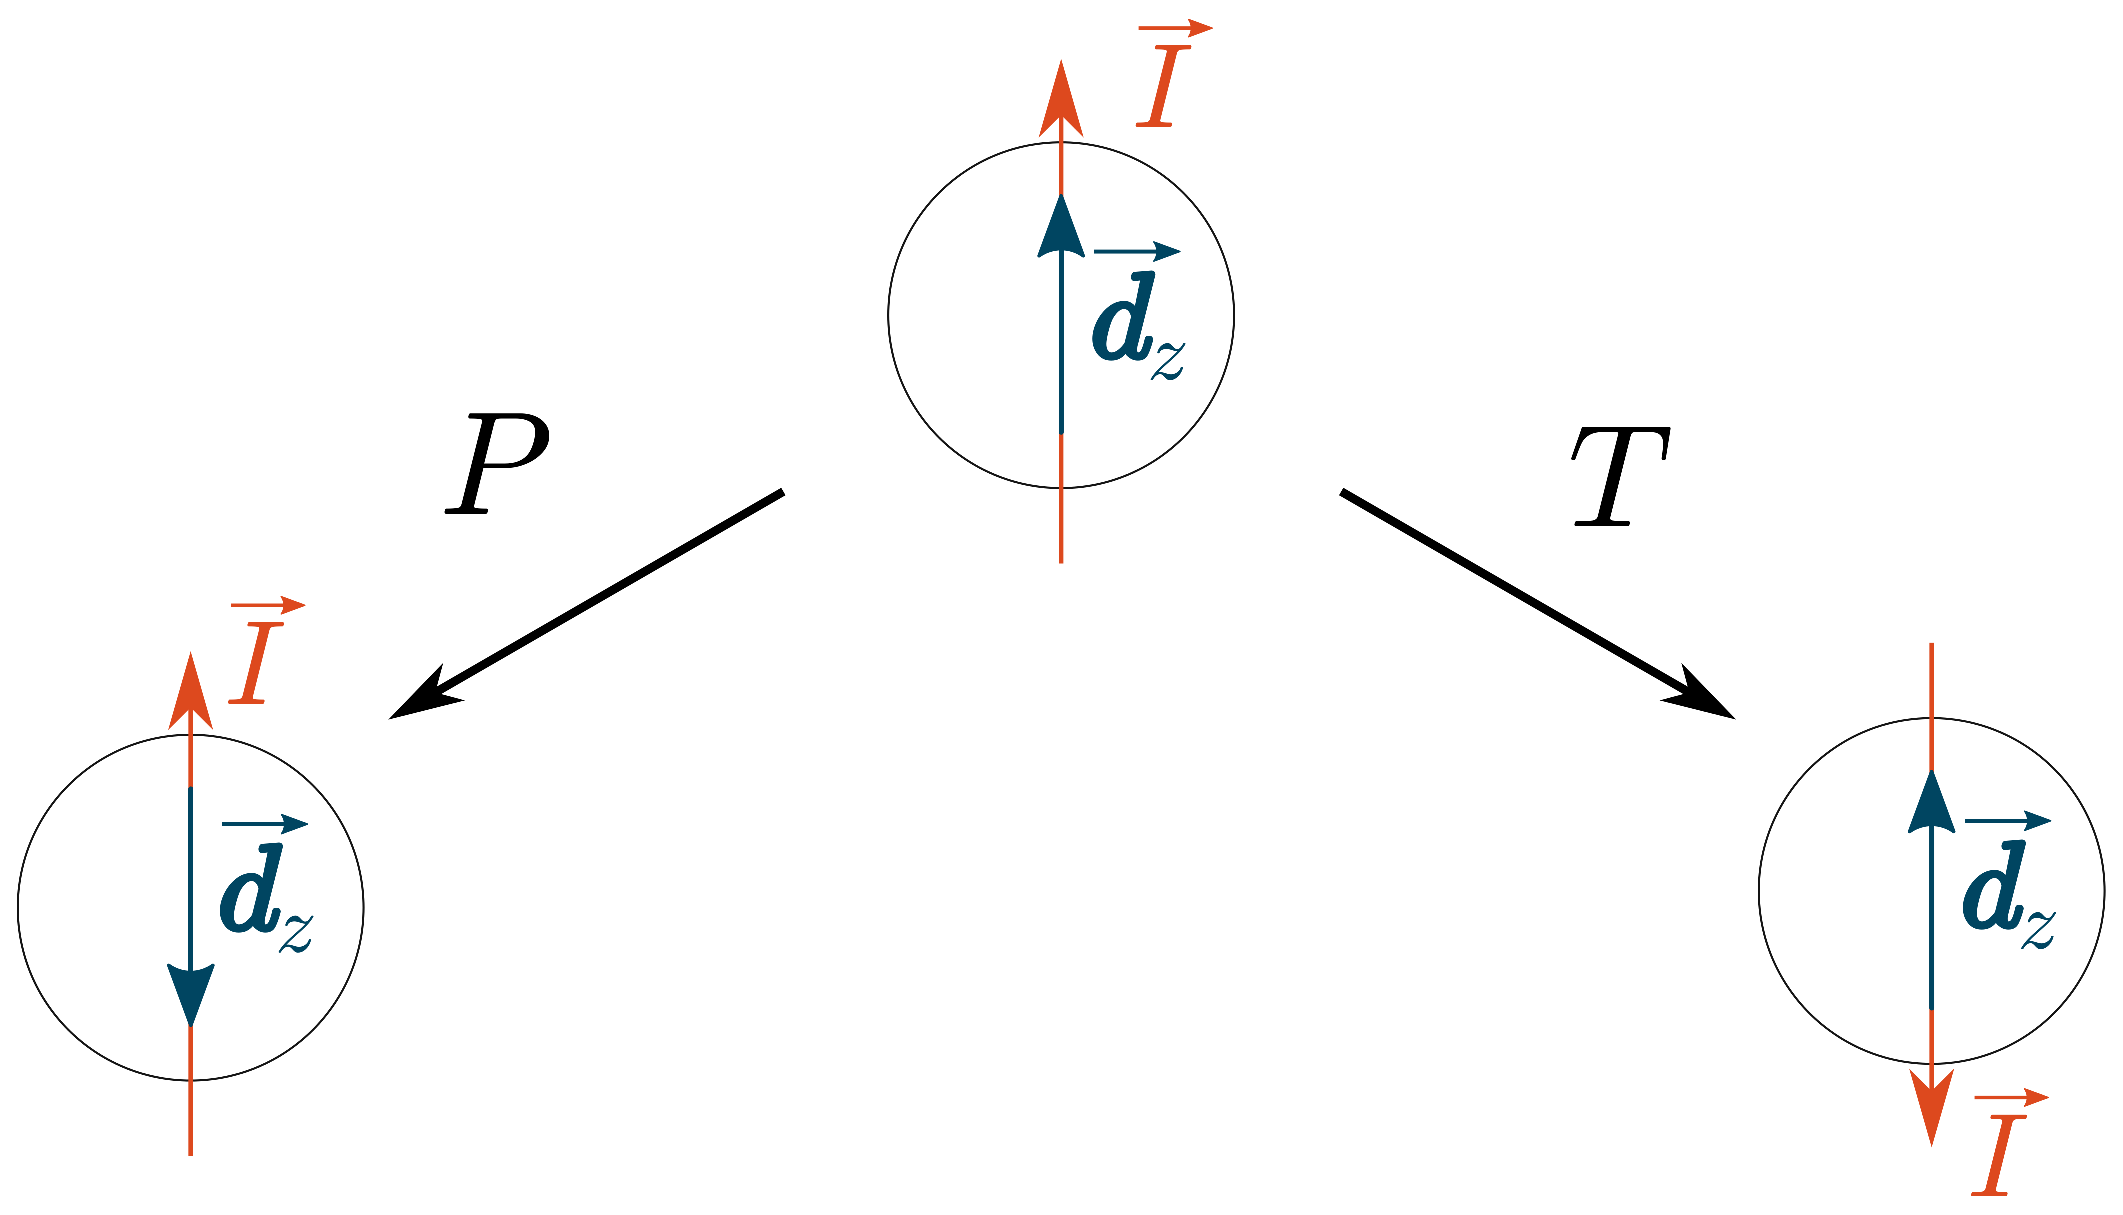
\includegraphics[scale=0.3]{./figures/EDM.eps}
\caption[Parity and time reversal transforms of a permanent EDM]{\label{fig:ParityTimeEDM} This diagram show the $P$ and $T$ transforms of a particle with angular momentum $I$ and a finite EDM $\textbf{d}$. The spatial EDM defined in  is $P$-odd and $T$-even. However as the EDM must be in the direction of the angular momentum of the particle which is $P$-even and $T$-odd there is a contradiction and the EDM violates $P$ and $T$.}
\end{figure}
Other than the EDM, other orders of permanent electromagnetic moments violate $T-$ symmetry. For the electric moments specifically, the next violating moment is the electric octupole moment (EOM). In terms of magnetic moments, the lowest order $T-,P-$ violating magnetic moment is the magnetic quadrupole moment (MQM) which has the form of a second order tensor. To demonstrate the $T-,P-$ violation of the MQM a similar argument to the EDM can be made when considering the two forms of the MQM tensor \cite{SFK1984},
\begin{align} \label{eq:MQMcurrent}
M_{kn} = - \int \left( r_k \epsilon_{npq} + r_n\epsilon_{kpq} \right)j_pr_q d^3r
\end{align}
\begin{align} \label{eq:MQMTensor}
M_{kn} = \dfrac{3}{2}\dfrac{M_{zz}}{I(2I-1)}\left[I_{k}I_{n} + I_{n}I_{k} - \dfrac{2}{3}I(I+1)\delta_{mk}\right].
\end{align}
Here $M_{zz}$ is the maximum value of the MQM on the $z$ axis, $\delta_{ij}$ and $\epsilon_{ijk}$ and the standard symmetric delta function and anti-symmetric tensor respectively. Equation (\ref{eq:MQMcurrent}) is both $T-$ and $P-$odd whereas equation (\ref{eq:MQMTensor}) is $T-$ and $P-$even, and therefore a permanent MQM violates both $T-$ and $P-$ symmetries. The MQM has more restrictive properties than the EDM as only systems with $I>1/2$ can have an MQM.\\
\linebreak
There has been considerable effort made to detect these $CP-$ violating moments over the last 60 years. Along with the proposal of a permanent EDM, Ramsey and Purcell along with Smith performed the first experiment to try and measure the EDM of a neutron \cite{Smith1957} where they set the first constraint on the neutron EDM. $d_n < 5 \times 10^{-20}$~cm. While this first experiment was performed on a free neutron, a promising avenue for measuring these moments is in atomic and molecular systems. In Section \ref{sec:ViolationInAtoms} we discuss the manifestation of $CP-$ violation in atomic and molecular systems specifically for the MQM. There has been a considerable amount of reviews on permanent EDMs and the violation of $CP-$ symmetry including references \cite{Barr1993, KhriplovichCP, GingesReview, Pospelov2005, LeptonMoments, Fukuyama2012, Engel2013, Jungmann2013, Roberts2015, Yamanaka2017, Safronova2018, Chupp2019}.
\section{Lorentz symmetry violation} \label{sec:Lorentz}
Like the discrete symmetries, Lorentz symmetry is one of the most fundamental symmetries in nature. It forms the basis of modern physics as a cornerstone of special relativity. Local Lorentz invariance (LLI) of a system states that there is no preferred reference frame of the universe and the laws of physics are unchanged when the orientation of the system (rotation) or speed of the system (boosts) is changed. Due to its importance, considerable effort has been made for over a century to test and quantify its validity through experiments \cite{Michelson1887, Kennedy1932, Ives1938, Robertson1949, LorentzTestSeries}.  \\
\linebreak
In the current SM, Lorentz invariance (along with combined CPT symmetry) is always conserved. However, there are many proposals for new physics BSM such as grand unified theories and string theories that require LLI to be violated \cite{Kostelecky1989,  Damour, Gambini1999, Pospelov2012, Kostelecky1995, Mavromatos2007, Liberati2013}.  Like the discrete symmetries, LLI is suspected to be a low-energy effective property which is spontaneously broken at higher energies due to an underlying theory. Unlike violation of the discrete symmetries however,  there  are no sources of LLIV in the SM and any measurement of some anisotropy will be the result of some unknown greater underlying theory. Therefore an extension to the SM in Refs. \cite{Colladay1997, Colladay1998, Kostelecky1999, LorentzDataTables2019} has been proposed which contains LLIV terms in the SM Lagrangian while preserving other desirable properties of the SM such as renormalizability and gauge invariance. This extension to the SM provides a framework to represent and quantify particular LLIV mechanisms in experiments. \\
\linebreak
Tests of Lorentz violation span both high-energy, cosmological scales down to low energy precision tests. The work in this thesis focuses only on its manifestation in low energy theory.  For a review of searches for LLIV in high energy tests see Ref. \cite{Coleman1999, Liberati2009, Stecker2012}.   \\
\linebreak
The possibility of observing new physics in low energy tests has led to a renewed concerted effort in detecting LLIV using modern experimental methods using more sophisticated techniques. These include  resonance cavity experiments \cite{Muller2005, Muller2003, Wolf2004}, Doppler shift experiments \cite{Lane2005, Saathoff2003} and clock comparison experiments \cite{Prestage1985, Chupp1989, Hohensee2013, Dzuba2016} (see Section \ref{sec:LorentzBound}). These experiments rely on measuring slight variations in results when the orientation or speed of the system is changed and therefore require extremely precise measurements. Currently, these experiments have only resulted in null measurements, however they have constrained the LLIV parameters in the SM extension (SME) extensively. A yearly review on the current status of LLIV can be found in \cite{LorentzDataTables2019} which provides an exhaustive list of the current constraints on LLIV parameters in the SM extension.\\
\linebreak
The SME proposed by D. Colladay and V. A. Kosteleck\'{y} is an exhaustive model containing all the Lorentz and CPT violating terms \cite{Colladay1997, Colladay1998, Kostelecky1999, LorentzDataTables2019} which also conserve renormalizability. The SM extension Lagrangian for a spin $\tfrac{1}{2}$ fermion is given by \cite{Colladay1997},
%\begin{align}
%\mathcal{L} = \dfrac{1}{2}i\bar{\psi}c_{\mu\nu}\gamma^{\mu}\overleftrightarrow{\partial^{\nu}}\psi.
%\end{align} 
\begin{align}
\mathcal{L} &= \dfrac{1}{2}i\bar{\psi}\Gamma_{\nu}\overleftrightarrow{\partial^{\nu}}\psi - M\bar{\psi}\psi. \label{eq:LLIVLagrangian} \\
\text{Where } \Gamma_{\nu} &= \gamma_{\nu} + c_{\mu\nu}\gamma^{\mu} + d_{\mu\nu}\gamma_{5}\gamma^{\mu} + e_{\nu} + i\gamma_5f_{\mu} + \dfrac{1}{2}g_{\lambda\mu\nu}\sigma_{\lambda\nu}, \nonumber \\
M &= m + a_{\mu}\gamma^{\mu} + b_{\mu}\gamma_{5}\gamma^{\mu} + \dfrac{1}{2}H_{\mu\nu}\sigma^{\mu\nu} \nonumber
\end{align}
, $f\overleftrightarrow{\partial^{\nu}}g = f\partial^{\nu}g - g\partial^{\nu}f$ and $\gamma_{\mu}$, $\gamma_5$ and $\sigma_{\mu\nu}$ are the standard Dirac and Pauli matrices. Where each of the parameters in $\Gamma$ and  $M$ (except the first terms which describe the current SM) are different parameters of Lorentz violating mechanisms.  In this thesis only consider the CPT-even Lorentz violating term associated with the momentum tensor $c_{\mu\nu}$. Constraints on all other LLIV parameters in (\ref{eq:LLIVLagrangian}) can be found in \cite{LorentzDataTables2019}. In Refs. \cite{Kostelecky1999, Hohensee2013} it was shown that the energy shift for a bound state of the fermion related to $c_{\mu\nu}$ by,
\begin{align} \label{eq:Lorentzshift}
\delta H = -mc_{00} + m\left(c_{0j} + c_{j0}\right)\dfrac{p_j}{m} + m\left(-c_{jk} - \dfrac{1}{2}c_{00}\delta_{jk}\right)\dfrac{p_ip_k}{m^2}.
\end{align} 
The LLIV parameter $C_{\mu\nu}$ represents the anisotropy in the maximal attainable speed (or kinetic energy) for particles in the matter sector (for example electrons, protons, neutrons). In this thesis only the last term of  Eq. (\ref{eq:Lorentzshift}) is studied  which relates to the momentum tensor $p_ip_j$. We discuss the potential measurement of this term in atomic and nuclear system in Section \ref{sec:ViolationInAtoms}. 
\section{Violation in nuclear, atomic and molecular systems} \label{sec:ViolationInAtoms}
As mentioned previously, while violation of the LLI, $P-$ and $CP-$ symmetries are spontaneously broken at extremely high energies, signatures of these violations may manifest at low energies. The low energy realm of atomic, molecular and nuclear physics is a perfect domain to search for these signatures as they offer high sensitivity at relatively low cost and provide an optimal space to test the Standard Model as all SM interactions are found in atomic theory. 
\subsection{The magnetic quadrupole moment}
While fundamental particles are expected to have intrinsic $CP$- violating permanent electrodynamic moments composite systems such as atoms, nuclei and baryons as expected to possess these net $CP-$ violating moments too. $CP-$ violations in composite systems can be interpreted as more fundamental parameters of $CP$- violating interactions in the lepton and quark-gluon sectors. For an in-depth review on symmetry violating electromagnetic moments including the MQM see Ref. \cite{GF2004, KhriplovichPNC, SFK1984, Roberts2015, KhriplovichCP, Pospelov2005}. The MQM of composite systems such as the deuteron \cite{Liu2012} have previously been investigated. The search for MQM has several advantages in comparison with the electrostatic $T,P$-violating moments (EDM, Schiff and octupole moments). For instance the nuclear EDM in neutral atoms and molecules is completely screened which is known as the Schiff theorem\cite{Schiff1963}. An analogous ``Schiff'' moment and octupole moment from the third order multipole expansion of the electrostatic field have an additional second power of a very small nuclear radius. Therefore the interaction of these electrostatic $CP-$ violating moments are suppressed. \\
\linebreak For the MQM the magnetic interaction is not screened and the contribution to the atomic EDM typically is an order of magnitude larger than the contribution of the Schiff moment and several orders of magnitude larger than the octupole contribution \cite{SFK1984, Flambaum1997}.  In quadrupole deformed nuclei MQM is enhanced by an order of magnitude \cite{Flambaum1994}, therefore, the MQM contribution to atomic EDM may be two orders of magnitude larger than the Schiff moment contribution. In the expression for the Schiff moment there is a partial cancellation between the first term and the second (screening) term. There is also a screening correction to the octupole moment \cite{ Flambaum1986, SFK1984, Flambaum2012}. In the Hg and Xe atoms  where the most accurate measurements of atomic EDM have been performed, the valence nucleon is a neutron. Therefore, the electrostatic moments (EDM, Schiff and octupole) moments do not appear directly, they exist due to the nuclear polarization effects \cite{Flambaum1986}. Due to the screening effect and the indirect polarization origin of the Schiff moment the nuclear calculations are rather unstable. In the case of the MQM moment both valence protons and neutrons  contribute directly, and the result is expected to be more accurate\cite{Flambaum2014}. Therefore the nuclear MQM moment is a good candidate for detecting $CP-$ violation, particularly for systems with large deformed nuclei (See Chapter \ref{chap:MQM}).\\
\linebreak
 A promising method of measuring $CP$- violating moments is in diatomic molecular experiments where the effective electric field is significantly larger than those directly accessible in laboratory experiments.  There is a considerable body of work for calculating the effective electric field in diatomic molecular systems which may be experimentally viable. Both theoretical and experimental progress has been made in measuring the $T,P-$ odd effects in  YbF\cite{Hudson2011, Mosyagin1998, Quiney1998, Parpia1998, Kozlov1994, Nayak2009, Steimle2007, Abe2014}, HfF$^+$ \cite{Cossel2012, Loh2013, Petrov2007, Fleig2013, Meyer2006, Skripnikov2008Hf, Le2013, Skripnikov2017Hf, Cairncross2017}, ThO \cite{Petrov2014, Meyer2008, Skripnikov2013ThO, Skripnikov2014ThO, Titov2015ThO, Fleig2014, Denis2016, Baron2017}, ThF$^+$\cite{Loh2013, Skripnikov2015Th, Denis2015}, TaN \cite{Skripnikov2015Ta, Fleig2016TaN} and TaO$^+$ \cite{Fleig2018} particularly in relation to the nuclear Schiff moment and electron EDM.   In section \ref{sec:MQMmolecule} we present the molecular energy shift due to the nuclear MQM for these molecules.\\
 \linebreak 
 The PNC effects appear due to mixing of opposite parity states in atoms and molecules by the weak interaction between the nucleus and electrons. The field  of PNC in atoms and molecules has been thoroughly reviewed in Refs.  \cite{KhriplovichPNC,GingesReview,RobertsReview}. It was noted in Ref.  \cite{FS78} that the nuclear quadrupole moment induces a tensor PNC weak interaction between the nucleus and electrons (see also  \cite{KhriplovichPNC,KP91}). In Ref. \cite{Flambaum2016} it was argued that these tensor  effects of the weak quadrupole moments are strongly enhanced for deformed nuclei and may get a significant additional enhancement due to mixing of  close atomic and molecular levels of opposite parity with a  difference of the electron angular momenta $|J_1-J_2| \le 2$. These selection rules are similar to that for the effects of the time reversal ($T$) and parity ($P$) violating nuclear magnetic quadrupole moment (MQM). Therefore, nuclei, molecules and molecular levels  suggested for the MQM search in Ref. \cite{Flambaum2014},  for example,  $|\Omega |=1$ doublets in the molecules $^{177}$HfF+, $^{229}$ThO, $^{181}$TaN will also have enhanced effects of the weak quadrupole (see section \ref{sec:PNC}). Following our proposal, there has been recent experimental interest in using the weak quadrupole moment to study PNC effects in HfF$^{+}$ molecules (used to measure electron electric dipole moment \cite{Cairncross2017}) and parity violation in $^{173}$Yb \cite{Antypas2017} and $^{163}$Dy \cite{Leefer2017} atoms. Molecules in particular present a lucrative option due to existence of very close paired levels of opposite parity, the  $\Omega$-doublet - see e.g.  \cite{Flambaum2014}. For highly polar molecules consisting of a heavy and light nucleus (for example, Th and O) the effect of MQM is $\sim Z^2$, therefore it is calculated for the heavier nucleus. The Hamiltonian of diatomic paramagnetic molecule including the $T, P-$ odd nuclear moment effects is given by \cite{SFK1984,Kozlov1995}:
\begin{align}
H = W_d d_e \mathbf{S}\cdot\mathbf{n} + W_{Q}\dfrac{Q}{I}\mathbf{I}\cdot\mathbf{n} - \dfrac{W_{M}M}{2I(2I -1)}\mathbf{S}\hat{\mathbf{T}}\mathbf{n},
\end{align}
where $d_e$ is the electron EDM, $Q$ is the nuclear Schiff moment, $M$ is the nuclear MQM, $\mathbf{S}$ is the electron spin, $\mathbf{n}$ is the symmetry axis of the molecule, $\hat{\mathbf{T}} $ is the second rank tensor operator characterised by the nuclear spins $T_{ij} = I_iI_j + I_jI_i - \tfrac{2}{3}\delta_{ij}I(I + 1)$  and  $W_d$, $W_Q$ and $W_M$ are fundamental parameters for each interaction which are dependent on the particular molecule. We have omitted the $P$-,$T$- odd electron-nucleon interaction terms which are presented e.g. in reviews \cite{Safronova2017,GF2004}. 
These parameters $W_d$, $W_Q$ and $W_M$
%, which are necessary for extracting the nuclear MQM from an experiment, 
are related to the electronic molecular structure of the state.
 
\subsection{Lorentz violation in bound systems} \label{sec:LorentzBound}
The developments of low energy precision measurements has constrained the LLIV parameters in equation (\ref{eq:LLIVLagrangian}) over the last  century \cite{LorentzDataTables2019}. Each of these constraints are categorized into different sectors depending on the manifestation of the Lorentz violation.  In this thesis we only consider LLIV in the matter sector. Equation (\ref{eq:Lorentzshift}) describes the energy shift of bound spin $\tfrac{1}{2}$ fermion and therefore detecting energy shifts in atomic electrons and nucleons are a prime avenue of low energy physics to detect LLIV. In fact, the best current laboratory limits are from clock comparison experiments \cite{Prestage1985, Chupp1989, Hohensee2013, Dzuba2016}. In particular, the $c_{\mu\nu}$ tensor parameter for the neutron was constrained in \cite{Smiciklas2011} using a $^{21}$Ne clock and for the proton in \cite{Wolf2006} using $^{133}$Cs clocks which was further constrained by 4 orders of magnitude in \cite{Flambaum2016}. These results in $^{21}$Ne were also used to constrain LLIV in the photon sector and in the Coulomb interaction in  Ref.\cite{FlambaumRomalis2017} . It should be noted that the $c_{\mu\nu}$ is frame dependent and to standardize the constraints of experimental results around the earth is specified by its value is some specific reference frame. This reference frame is chose to be the Sun-centered, celestial equatorial frame defined in \cite{LorentzDataTables2019, Bluhm2002}. The spatial directions of this frame are represented by $X,Y$ and $Z$ and the temporal component is represented by $T$. All LLIV experimental constraints are projected onto this standard reference frame for comparison. For the tensor parameter $c_{\mu\nu}$ there are 9 total constraints with 5 being spatial only. Experiments testing LLIV need to be performed over long periods of time to observe slight variations.\\
\linebreak
Two types of atomic and nuclear experiments used to measure LLIV effects are clock comparison experiments and nuclear comagnetor (NMR) experiments. Clock-comparison experiments aim to detect changes in the energy transitions between states of bound electrons as the orientation of the system changes. Comagnetometer experiments aim to detect changes in the NMR frequency of nuclei for different orientations, however in order to constrain $c_{\mu\nu}$ parameter nuclei with $I>1/2$ must be used. The best constraints on $c_{\mu\nu}$ is the electron sector comes from a clock comparison experiments with dysprosium \cite{Hohensee2013}. To measure LLIV in the proton and nuetron sector comagnetor experiments have been implemented. \\
 \linebreak
Violation of LLIV in nuclear systems using the tensor interaction does not require study of nuclear transitions like other LLIV parameters as the angular momentum projections are different. The $C_0^{(2)} = c_{xx} + c_{yy} - 2c_{zz}$ is the LLIV tensor interaction in the laboratory frame where the quantization axis (same as the deformation axis deformed nuclei, see next chapter) lies along the $z$ axis. In Chapter \ref{chap:WQM} we calculate the LLIV energy shift for selection of promising deformed nuclei of experimental nuclei using the Nilsson model for quadrupole deformed nuclei (see \ref{chap:Deformed}). 
\subsection{Parity non conservation}
The violation of parity (not accompanied by $T-$ violation) in atomic and molecular systems has been a rich field of physics for decades. The primary source of parity violation in these systems is due to the $Z^0$ boson exchange between nucleons and electrons. A smaller electron-electron interaction is also present, though it is insignificant in comparison. The $P-odd$ weak interaction between the electrons and nucleons is given by
\begin{align*}
H_W = \dfrac{-G_F}{2\sqrt{2}} \gamma_5 \left[Zq_{w,p}\rho_{p}\left(r\right) + Nq_{w,n}\rho_{n}\left(r\right)\right]
\end{align*}
where $G_F$ is the Fermi-weak constant,$q_{w,p} $ and $q_{w,n} $ are the weak charges for the proton and nucleons respectively. The nucleon densities $\rho_p$ and $\rho_n$ are normalized to one. 
\begin{align*}
\int \rho_{n}\left(r\right) d^3r = 1.
\end{align*}
The magnitude of this interaction is scaled by the weak charges of the nucleons. Not including radiative corrections, these weak charges are given by \cite{KhriplovichPNC},
\begin{align*}
q_{w,p} &= 1 - 4\sin^2\theta_W \approx 0.08 ,\\
q_{w,n} &= -1,
\end{align*}
where $\theta_W$ is the Weinberg angle. As the complete weak charge is dominated by the neutron contribution, the total weak charge of the nucleus approximately scales with the neutron number with the number of protons as a small correction, $Q_{w} \approx N$.\\
\linebreak
This interaction is purely scalar, and therefore it will only mix states with the same angular momentum. There has been considerable study on the vector interaction which will mix state of angular momentum which differ by at least 1. This vector interaction is dominated by the $P-$odd nuclear anapole moment \cite{GingesReview}. The nuclear anapole moment lies outside the scope of this thesis and we will not consider it further. For more information refer to the reviews \cite{GingesReview, Roberts2015, KhriplovichPNC}. \\
\linebreak
While the scalar and vector weak interactions have been considered deeply in the literature, little work has been done on higher order interactions. In this thesis we introduce the weak quadrupole moment (WQM) of the nucleus (Chapter \ref{chap:WQM}) which will mix atomic states of angular momentum $\Delta J = 2$. To understand this second order tensor interaction a greater understanding of the quadrupole distribution of nucleons in the nucleus is required. While the proton distribution is well-studied and understood experimentally, determination of the neutron quadrupole distribution is difficult and current experimental techniques are not sensitive to this distribution.  
\chapter[Properties of deformed nuclei]{Properties of deformed \\ nuclei} \label{chap:Deformed}
 In this chapter I give a brief overview of the Nilsson model for deformed nuclei and the quadrupole properties of second order tensors in nuclei.

\section{Quadrupole deformation of nuclei} 
In this thesis only quadrupole deformations are considered. There are two types of quadrupole deformations. The first are prolate deformations where the nuclear matter is concentrated around the axis of deformation (See Figure \ref{fig:defnuclei}). The second type are oblate deformations where the nuclear matter is aligned perpendicular to the deformation axis. The existence of non-spherical nuclei has been suspected since the 1930s where anomalous behaviour was observed in the hyperfine structure in isotopes of Eu ($Z=63$) and Lu ($Z=71$) by H. Schuler and Th. Schmidt \cite{Schuler1935(1), Schuler1935(2)}. Soon after this discovery, H.~B.~G.~Casimir published an explanation of these results and posited the anomaly could be explained by the existence of an permanent electric quadrupole moment of the nucleus which interacts with the atomic electrons \cite{Casimir1935, Casimir1936}. The origin of this nuclear quadrupole moment was originally ascribed to the existence of an unpaired valence nucleon with nuclear spin $I_t$ which induces an electric quadrupole moment  $Q_{p,\text{val}}$ of the nucleus by the equation \cite{BohrMottVol1},
\begin{align}\label{eq:valQ}
Q_{p,\text{val}} &=  - \dfrac{I_t-1/2}{I_t + 1}0.009A^{2/3} \ \text{barn}.
\end{align}  
This single particle description is incomplete for several reasons. The magnitude of a quadrupole moment from a single proton is significantly less than those observed in experiment. For example consider $^{181}_{73}$Ta, which has total nuclear spin $I_t=7/2^{+}$, using equation (\ref{eq:valQ}) results in a quadrupole moment of $Q_{p,\text{val}} = -0.192 \ \text{barn}$. This is significantly less (along with opposite sign) than the experimental $Q_p = +3.17(2) \ \text{barn}$. Therefore the quadrupole moment of a nucleus must be a collective effect of the nucleus involving a large amount of the nuclear matter and cannot be accounted for by a single nucleon and the neutron quadrupole moment of the nucleus (NQMN) must be considered. \\
\linebreak
Unlike $Q_p$ which can be measured through the study of hyperfine structure in element spectroscopy, measuring the NQMN, $Q_{n}$,  is a very difficult  task as neutrons are electrically neutral particles. The NQMN is an important property which will give insight not only into the structure of  atomic nuclei but also other dense collections of neutrons such as neutron stars \cite{Brown2000, Furnstahl2002, Typel2001, Reinhard2010} and also the theory of atomic parity nonconservation. For the last two decades there has been increasing interest in understanding the distribution of neutrons compared to protons in atomic nuclei known as the neutron skin. This focus has largely been on the spherical distribution of neutrons (measurement of the root mean square radius of neutrons) and there has been a large amount of experimental effort in measuring the spherical distribution \cite{Clark2003, Trzcinska2001, Lenske2009, Abrahamyan2012}. To understand these quadrupole properties we consider the Nilsson model of the nucleus.
  \begin{figure}
\centering
\begin{subfigure}[b]{0.48\textwidth}
\centering
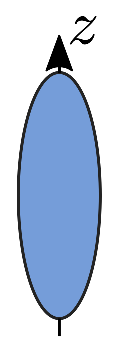
\includegraphics{./figures/prolate.eps}
\caption{Prolate deformation of a nucleus. Here the $z$ axis is the symmetry axis.}
\end{subfigure}	
\quad
\begin{subfigure}[b]{0.48\textwidth}
\centering
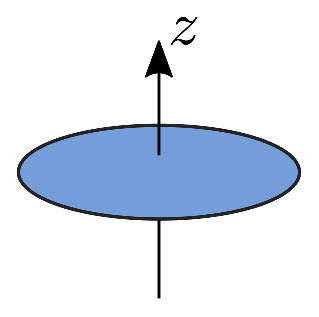
\includegraphics{./figures/oblate.eps}
\caption{Oblate deformation of a nucleus. Here the $z$ axis is the symmetry axis.}
\end{subfigure}
\caption[Quadrupole deformations of nuclei]{ \label{fig:defnuclei}}
\end{figure}
\section{The Nilsson Model}
  The independent particle model only describes how a single nucleon will behave in a mean field. In the case of an atom this is a relatively simple and stable approach. To a first approximation, the atomic electrons experience a potential from the much larger point like nucleus. It is only in higher approximations that  the inter electron potential is treated by using methods such as Hartree-Fock. However in the nucleus there is no centre source of potential, it all comes from the inter-nucleon interactions which are a complex interplay of the Coulomb and the strong force and is not completely understood. Therefore any mean field potential ascribed to the nucleus is going to be inherently unstable, especially when considering larger nuclei. This results in a anisotropy of the nucleus which has interesting properties when trying to understand nuclear physics. Therefore to consider deformations in nuclei anisotropic nuclear models need to be considered in addition to the isotropic case. \\
\linebreak
While collective effects of the nucleus had been considered for a significantly long time with the liquid drop model, they were not considered in the context of the microscopic prospect of the nucleus\cite{Brix1986}. The isometric (spherical) shell model is an independent single particle model where the nucleons are modeled in a mean field approximated by the interaction of the other nucleons which was very successful in predicting the closed shells in spherical nuclei\cite{Mayer1949, Jensen1949}. While the spherical shell model was successful in predicting closed shell of spherical nuclei, it had limitations when considering highly deformed nuclei. Collective properties of the nucleus include large quadrupole moments and nuclear fission. Non-spherical nuclei were first explored in depth by Rainwater in 1950 \cite{Rainwater1950}. A single-particle model which accounts for the asymmetry of the nucleus was developed by S. G. Nilsson in 1955 \cite{Nilsson1955}. This model, known as the Nilsson model, uses an anisiotropic harmonic oscillator potential to describe the nuclear potential the nucleons move in. The complete Hamiltonian of the Nilsson model is given by \cite{Nilsson1955, Gustafson1967},
\begin{align} \label{eq:NilssonHamiltonian}
H = \dfrac{\textbf{p}^2}{2m} + \dfrac{1}{2}m \left[\omega_{\perp}\left(\textbf{x}^2 + \textbf{y}^2\right) + \omega_z \textbf{z}^2\right] + C\textbf{l}\cdot \textbf{s} + D \left(\textbf{l}^2 - \left<I^2\right>\right)
\end{align}
which has the form of an asymmetric three dimensional harmonic oscillator model where we have chosen the $z-$axis as the axis of deformation. Here $m$ is the nucleon mass, $\omega_z$ and $\omega_{\perp} = \omega_x = \omega_y$ (as we are considering quadrupole deformations only) are the nucleon oscillation frequencies along the $z-$axis and the perpendicular  plane respectively.  Both the spin-orbit term ($\textbf{l}\cdot \textbf{s}$) and the  $\textbf{l}^2 - \left<I^2\right>$ terms were included to reproduce the magic numbers in the spherical limit. Specifically, the $\left<I^2\right>$  term was introduced phenomenologically to correct the energy of the single-particle states closer to the nuclear surface and lower them to correct for the steep rise in the harmonic-oscillator potential there. 	To relate this Hamiltonian to a collective deformation of the nucleus, $\delta$, the angular frequencies and deformation parameter are related by,
\begin{align*}
\omega_{\perp^{2}} = \omega_0^2\left(1 + \dfrac{2}{3}\delta\right) \\
\omega_z^2 = \omega_0^2\left(1 - \dfrac{4}{3}\delta\right)
\end{align*}
\linebreak
In the spherical shell model the orbit with angular momentum $I$ has degeneracy $2I + 1$ nucleons. This degeneracy is broken in the Nilsson model for deformed nuclei where the projection of the angular momentum onto the symmetry axis, $\Omega$, is the good quantum number (see Figure \ref{fig:prolate_AM}). Each of these $\Omega$ states are doubly degenerate. The consequences of a deformed nucleus on the quantum states of the constituent nucleons can be deduced from two simple physical arguments. Consider the non-rotating, intrinsic (body) frame of the nucleus. Where $\Omega$ is the projection of the nucleons angular momentum $I$ on the deformation axis. 
\begin{figure}
\centering
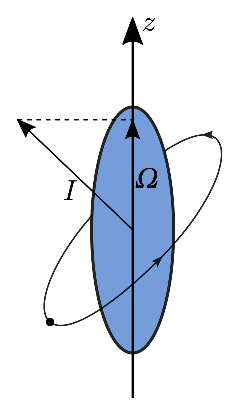
\includegraphics[scale=1]{./figures/prolate_AM.eps}
\caption[Angular moment projections in deformed nuclei]{Projection of angular momentum of a prolate deformed nucleus onto the symmetry axis in the intrinsic frame. Here $I$ is the angular momentum of the nucleon and $\Omega$ is its projection on the axis of deformation.}
\label{fig:prolate_AM}
\end{figure}
By definition the projection of total angular momentum on the symmetry axis $\Omega$ is the sum of the projection of the orbital angular momentum, $\Lambda$ and the projection of the spin angular momentum $\Sigma = \pm 1/2$,  $\Omega = \pm\tfrac{1}{2}, \pm\tfrac{3}{2},  \pm\tfrac{5}{2},  ... ,  \pm\tfrac{I}{2}$.\\
\linebreak
%\begin{align*}
%\delta \approx 0.95 \beta
%\end{align*}
The deformation of the nuclear field implies important modifications of the nucleonic motion. Each orbit may be occupied twice, corresponding to the two possible signs of $\Omega$. The absence of degeneracies implies a very simply coupling scheme for the particle motion. In the regions of closed major shells ($N$) the equilibrium shape of the nucleus is spherical. The only oblate candidates are those where the protons or neutrons are near the end of a major shell. Therefore the vast majority of nuclei are prolate deformed. To classify each constituent nucleon in the deformed nucleus we use the notation proposed by Nilsson\cite{Nilsson1955, BohrMottVol2}. Each nucleon can be characterized by the set of quantum numbers $\left[N n_z \Lambda \pm\Omega\right]$ \cite{BohrMottVol2}  where $N = n_z + n_x + n_y$ and each $n_i$ ($i = x, y, z$) is the principal quantum number in the direction of $i$, $\Lambda$ and $\Omega$ are the nucleon's orbital and total angular momentum projection on the deformation axis respectivly. Each energy level is doubly degenerate for $\pm\Omega$. The average oscillator frequency is given by $\hbar\bar{\omega} = \hbar/3\left(2\omega_{\perp} + \omega_z\right) \approx 45A^{-1/3} - 25A^{-2/3} \ \text{MeV}$\cite{Brown2016}. 
\section{Second order tensor properties of nuclei}
Second order tensor properties  in deformed nuclei exhibit a collective enhancement compared to vector properties. Consider the magnetic dipole moment  which is proportional to  the projection of the total angular momentum $\Omega$ to the nuclear axis. In an even-even nucleus all the nucleons are paired and therefore the magnetic dipole moment of the $+\Omega$ state cancels with the $-\Omega$ state resulting in no net magnetic dipole moment of the nucleus. For an odd $A$ nucleus  the magnetic dipole moment of the entire nucleus is simply the dipole moment of the odd nucleon. This is the well known Schmidt model of the nucleus. The cases for second order tensor properties of the nucleus are different. For  nucleons in the  $+\Omega$ and the $-\Omega$ states tensor properties  are additive. Therefore there is a collective effect and many nucleons contribute to the tensor properties of the nucleus.\\
\linebreak
In the Nilsson model we consider the nucleus in the intrinsic frame which rotates with the nucleus. However the nucleus itself rotates with respect to the fixed laboratory frame \cite{BohrMottVol2}. Due to this rotation, the tensor properties transform between the intrinsic  and laboratory frame. The relationship between these two frames is \cite{BohrMottVol2}
\begin{align} \label{eq:RotationalFactor}
A^{Lab} = \dfrac{I\left(2I - 1\right)}{\left(I + 1 \right)\left(2I + 3\right)}A^{Intrinsic},
\end{align}
where $I=I_z= \left|\Omega\right|$ is the projection of total nuclear angular momentum (nuclear spin) on the symmetry axis. This expression shows that only in nuclei with spin $I > 1/2$ can we detect these second order tensor properties. \\
\linebreak
In Chapters \ref{chap:WQM} and \ref{chap:MQM} we calculate the second order properties NQMN, LLIV tensor and the MQM for several nuclei of experimental interest using the Nilsson model.
\chapter[The weak quadrupole moment and Lorentz violation in nuclei ]{The weak quadrupole moment and Lorentz violation in \\ nuclei} \label{chap:WQM}
Non-spherical nuclei present a lucrative avenue for studying the existence and magnitude of second order tensor properties due to the collective properties of deformed nuclei. In this chapter we focus on the quadrupole moment of the nonspherical  distribution of neutrons in the nucleus, $Q_{n}$,  the weak quadrupole moment (WQM), $Q_{W}^{(2)}$,  and the violation of Local Lorentz invariance (LLI) in the nucleon sector. The results of this chapter have been published in Ref. \cite{LFWQM2018}.

\section{Quadrupole moment of neutron distribution in deformed nuclei}
The quadrupole moment tensor along the symmetry axis of the nucleus in cartesian coordinates is given by
\begin{align}\label{eq:QMomentStandard}
Q_{zz} = Q = 2\left<z^2\right> - \left<x^2\right> - \left<y^2\right> .
\end{align}
From the virial theorem for bound particle in a harmonic oscillator potential the average kinetic energy $\left<T\right>$ and average potential energy $\left<U\right>$ are equal. Using the well known energy spectrum for the harmonic oscillator $E_{n} = \hbar\omega(n + 1/2)$  the average of the square of the position in the $z$ direction is,
\begin{align}\label{eq:zExpectation}
m\omega_z^2\left<z^2\right>&= \hbar\omega_z\left(n_z + 1/2\right) 
\end{align}
  with similar relations for $\left<x^2\right>$ and $\left<y^2\right>$. Using equations (\ref{eq:QMomentStandard}), (\ref{eq:zExpectation}) and $n_x + n_y = N - n_z$ the contribution to the quadrupole moment from a single nucleon in the quantum state $\left[N n_z \Lambda \Omega\right]$ is given by
\begin{align} \label{eq:QMomentNucleon}
q_{i,\nu} &= \dfrac{\hbar}{m}\left[\dfrac{\left(2n_z + 1\right)_{i,\nu}}{\omega_z} - \dfrac{\left(N -n_z + 1\right)_{i,\nu}}{\omega_{\perp}}\right] ,
\end{align}
where $\nu = p,n$ for the $i$th proton or neutron respectively. The total quadrupole moment is the sum of all the respective nucleon quadrupole moment contributions
\begin{align}
Q_{\nu} &= \sum_{i} q_{i,\nu} \nonumber\\
&= \dfrac{\hbar}{m}\left[\dfrac{1}{\omega_z}\sum_{i}\left(2n_z + 1\right)_{i,\nu} - \dfrac{1}{\omega_{\perp}}\sum_{i}\left(N -n_z + 1\right)_{i,\nu}\right]. \label{eq:CollectiveMDim} 
\end{align}
\section[Lorentz invariance violation  in deformed nuclei]{Lorentz invariance violation  in deformed \\ nuclei} 
In reference \cite{Brown2016} the $s-d$ shell model calculations of the tensor LLIV effects have been performed in $^{21}$Ne, $^{131}$Xe and $^{201}$Hg nuclei. It was demonstrated that virtual excitations from the nuclear core enhance the nuclear quadrupole moment and suppress the LLIV tensor.  The results of the $s-d$ shell model calculations have been supported by the calculations in the Hartree-Fock-Bogoliubov model published in the same paper \cite{Brown2016}.\\
\linebreak
The LLIV momentum tensor Hamiltonian, $\delta H$, is given by  \cite{Kostelecky1999}
\begin{align} \label{eq:HamilQuadShift}
\delta H = \left[-c_{ij} -\dfrac{1}{2}c_{00}\delta_{ij}\right]\dfrac{p_ip_j}{m^2},
\end{align}
 where $m$ is the nucleon mass,  to describe the tensor parameter $c_{ij}$  for the LLIV interaction \cite{Kostelecky1999} in the laboratory frame. 
Taking the expectation value of equation (\ref{eq:HamilQuadShift}), we find that the LLIV energy shift  for a nucleus with $N_{\nu}$ nucleons with angular momentum projection $I_{\nu}$ is given by 
%\cite{Kostelecky1999},
\begin{align} \label{eq:MomentumEnergyShift}
<\delta H>_{\nu} = \dfrac{1}{6m}C_{0, \nu}^{(2)}\sum_{N=1}^{N_{\nu}}\left<I_{\nu},I_{\nu}\left|\hat{M}\right|I_{\nu},I_{\nu}\right> 
\end{align}
where the $\hat{M} = 2\hat{p}_z^2 - \hat{p}_x^2 - \hat{p}_y^2$ is the momentum tensor operator for $p_ip_j$ in the SME in cartesian coordinates. We use the standard notion $C_{0, \nu}^{(2)} = c_{xx} + c_{yy} -2c_{zz}$ \cite{Kostelecky1999}. We define the single nucleon LLIV momentum tensor as
\begin{align} \label{eq:LLIVMomentum}
\bar{m}_{i, \nu} =  \left<I,I\left|2\hat{p}_z^2 - \hat{p}_x^2 - \hat{p}_y^2\right|I,I\right>.
\end{align}
Using the virial theorem for a harmonic oscillator ($\left<T\right>=\left<U\right>$) and energy spectrum again we have the average square of the momentum given by
\begin{align} 
\dfrac{\left<p_z^2\right>}{2m} &= \dfrac{\hbar\omega_z\left(n_z + 1/2\right)}{2} \label{eq:pExpectation}
\end{align}
with similar expressions for $x$ and $y$ coordinates. \\
\linebreak
Using equations (\ref{eq:LLIVMomentum}) and (\ref{eq:pExpectation}) we write the contribution to the LLIV tensor of a nucleon as,
\begin{align} \label{eq:MDimensionful}
\bar{m}_{i,\nu} &= \hbar m\left[\left(2n_z + 1\right)_{i,\nu}\omega_z - \left(N - n_z + 1\right)_{i,\nu}\omega_{\perp}\right].
\end{align}
The total LLIV tensor, $M_{\nu}$,  for the nucleus is the sum of all respective nucleons
\begin{align}
M_{\nu} &= \sum_{i,\nu} \bar{m}_{i,\nu} \nonumber \\
&= \hbar m\left[\omega_z\sum_{i}\left(2n_z + 1\right)_{i,\nu} - \omega_{\perp}\sum_{i}\left(N - n_z + 1\right)_{i,\nu}\right]. \label{eq:CollectiveQDim}
\end{align}
This will result in a quadrupole energy shift given by
\begin{align} \label{eq:LLIVEnergyShift}
\left<\delta H\right>_{\nu} = \dfrac{M_{\nu}}{6m} C_{0,\nu}^{(2)}.
\end{align}

\begin{align}
Q_{\nu} = \dfrac{41.5\text{ MeV}\text{fm}^2}{\hbar\bar{\omega}}\left[\eta\sum_{i}\left(2n_z + 1\right)_{i,\nu}  - \xi\sum_{i}\left(N - n_z + 1\right)_{i,\nu}\right]&
\label{eq:QDimensionless}
\end{align}
\begin{align}
M_{\nu} = \hbar\bar{\omega}m\left[\dfrac{1}{\eta}\sum_{i}\left(2n_z + 1\right)_{i,\nu} - \dfrac{1}{\xi}\sum_{i}\left(N - n_z + 1\right)_{i,\nu}\right]. & \label{eq:MDimensionless}
\end{align}
Rewriting equations (\ref{eq:CollectiveMDim}), (\ref{eq:CollectiveQDim})  and, the relation between the longitudinal  and perpendicular frequencies in dimentionless quantities $\eta = \bar{\omega}/\omega_z$ and $\xi = \bar{\omega}/\omega_{\perp}$ we have the equations,
\begin{align}
3 &= \dfrac{1}{\eta} + \dfrac{2}{\xi} \label{eq:average} 
\end{align}
The nucleon angular momentum dependence shows up in the order of the split energy branches in the Nilsson plots \cite{Nilsson1955, BohrMottVol2}.
%It should be noted that there is no explicit dependence on the angular momentum of the nucleons. This is because the angular momentum dependence is in the order of the nucleons in the Nilsson plots used to find the nucleonic configuration. 
The parameters $\eta$ and $\xi$ can be viewed as deformation parameters of the nuclei. For positive deformation $\eta > 1$ (prolate) and for negative deformation $\eta < 1$ (oblate). As there is a predominance on nuclear prolate deformations in nature most of the nuclei we consider will be prolate. \\
\linebreak
We indirectly include spin-orbit and angular momentum terms of the Nilsson Hamiltonian through the split level Nilsson energy plots in ref. \cite{BohrMottVol2}.
The collective enhancement of MQM for some  heavy deformed nuclei were estimated in \cite{Flambaum1994, Flambaum2014} where they considered the contribution using a spherical wave function basis. 
\section{Example calculation of $Q_{\nu}$ and $M_{\nu}$ for the $^{173}$Yb nucleus}
To illustrate the process of calculating NQMN and LLIV values we will present the calculation of $^{173}$Yb. To begin we find the nuclear configuration of protons and neutrons in the deformed field using the energy level plots presented in \cite{Nilsson1955,BohrMottVol2} (see Appendix \ref{chap:Nilsson}) by filling each non-degenerate $\Omega$ energy branch with two nucleons until all the nucleons have been distributed. To find the correct deformation, $\delta$, from which to fill we use the experimental value of the nuclear spin (which is solely due to the unpaired nucleon). The filling must be done such that the unpaired nucleon is in the correct spin state. The nuclear spin of $^{173}$Yb is $5/2^{-}$ due to an unpaired neutron. Using the method described above we find that this is possible with a minimum deformation of $\delta \approx 0.3$. Here we will only present the configuration of the partially filled $N$ shells. The numbers for each full shell are presented in the Appendix \ref{chap:Nilsson} (Table \ref{table:FullShellNz}). The incomplete neutron and proton shells in $^{173}$Yb are $N = 5,6$ and $N = 4,5$ respectively. The nucleon configuration of the incomplete shells are given in Table \ref{table:YbConfig}.
\begin{landscape}
\begin{table} 
\centering
\caption[Nilsson configuration of $^{173}$Yb nucleons in partially filled major shells.]{Nilsson configuration of $^{173}$Yb nucleons: This table shows the nuclear configuration of nucleons in the Nilsson model for $^{173}$Yb generated from the Nilsson plots in Ref. \cite{BohrMottVol2}. This table shows only partially filled $N$ shells. All preceding shells are completely filled. \label{table:YbConfig}}
\begin{tabular}{p{1.5cm}lcc@{\hspace{1cm}}p{1.5cm}lcc}
\toprule
\toprule
\multicolumn{2}{c}{\parbox[c][][c]{2cm}{\vspace{3pt}Neutrons in incomplete shells\vspace{3pt}}} & $\sum \left(2n_z + 1\right)_n$ & $\sum \left(N - n_z + 1\right)_n$ & \multicolumn{2}{c}{\parbox[c][][c]{2cm}{\vspace{3pt}Protons in incomplete shells\vspace{3pt}}} & $\sum \left(2n_z + 1\right)_p$ & $\sum \left(N - n_z + 1\right)_p$\\ 
\midrule
 $2f_{7/2}$: &\parbox[c][][l]{2cm}{\begin{flushleft}
 $\pm 1/2[530]$, $\pm 3/2[521]$, $ \pm 5/2[512]$\end{flushleft} }&  30 & 24 & $1g_{7/2}$: & \parbox[c][][c]{2cm}{\begin{flushleft}
$\pm 1/2[431]$, $\pm 3/2[422]$, $ \pm 5/2[413]$
\end{flushleft} }& 30 & 18 \\
 $1h_{9/2}$: &  \parbox[c][][c]{2cm}{\begin{flushleft}
 $\pm 1/2[541]$, $\pm 3/2[532]$, $ 5/2[523]$\end{flushleft} } & 37 & 14 & $2d_{5/2}$: & \parbox[c][][c]{2cm}{\begin{flushleft}
 $\pm 1/2[420]$, $\pm 3/2[411]$ \end{flushleft} } & 16 & 14 \\
 $3p_{3/2}$: & \parbox[c][][l]{2cm}{\begin{flushleft}
$\pm 1/2[521]$\end{flushleft}} & 10 & 8 & $2d_{3/2}$: & \parbox[c][][c]{2cm}{ \begin{flushleft}
$\pm 1/2[521]$ \end{flushleft} } & 6 & 8 \\
 $1h_{11/2}$: & \parbox[c][][c]{2cm}{\begin{flushleft}
 $\pm 1/2[550]$, $\pm 3/2[541]$, $\pm 5/2[532]$, $\pm 7/2[523]$, $\pm 9/2[514]$, $\pm 11/2 [505]$\end{flushleft}}   & 72 & 42 & $1g_{9/2}$: &  \parbox[c][][c]{2cm}{\begin{flushleft}
$\pm 1/2[440]$, $\pm 3/2[431]$, $ \pm 5/2[422]$, $\pm 7/2[413]$, $\pm 9/2[404]$ \end{flushleft} }  & 50 & 30 \\
 $1i_{13/2}$: & \parbox[c][][l]{2cm}{\begin{flushleft}
 $\pm 1/2[660]$, $\pm 3/2[651]$, $\pm 5/2[642] $, $\pm 7/2[633]$\end{flushleft}} & 80 & 20 & $1h_{11/2}$: & \parbox[c][][l]{2cm}{\begin{flushleft}
$\pm 1/2[550]$, $\pm 3/2[541]$, $\pm 5/2[532]$, $\pm 7/2[523]$ \end{flushleft} } & 64 & 20 \\  
\multicolumn{2}{c}{Total} & 229 & 108 & \multicolumn{2}{c}{Total}& 166 & 90  \\
\bottomrule
\bottomrule
\end{tabular}

\end{table}
\end{landscape}
Summing up the contribution for all the $^{173}$Yb filled shells and the partially filled shells from Table \ref{table:YbConfig} the total values for neutrons are $\sum(2n_z + 1)_{n} = 439$, $\sum(N - n_z + 1)_n = 318$ and protons $\sum(2n_z + 1)_{p} = 266$, $\sum(N - n_z + 1)_p = 190$. Using equation (\ref{eq:RotationalFactor}) to transform the measured value of the quadrupole moment in the lab frame $Q_p^{Lab} = 4.39$ barn (where 1 barn = 100 fm$^2$ = $10^{-24}$ cm$^{2}$) to the internal (rotating) frame we have $Q_{p}^{int} = 12.66\ \text{barn}$. Using equation (\ref{eq:QDimensionless}), the values for $\sum\left(2n_z + 1\right)_{p}$, $\sum\left(N - n_z + 1\right)_p$ and $Q^{int}_p$ we find the dimensionless deformation parameters $\eta = 1.18$ and $\xi = 0.93$ for $^{173}$Yb. Using equations (\ref{eq:QDimensionless}) and  (\ref{eq:MDimensionless}) to calculate the total NQMN and LLIV momentum tensors in the intrinsic frame, and equation (\ref{eq:RotationalFactor}) to transform back to the laboratory frame we find,
\begin{align*}
Q_{n}^{\text{Lab}} &= 4.53 \text{ barn} \\
M_{p}^{\text{Lab}} &= 54.30 \quad m\text{ MeV}\\
M_{n}^{\text{Lab}} &= 77.25 \quad m\text{ MeV}
\end{align*}
for the $^{173}$Yb. 
From equation (\ref{eq:LLIVEnergyShift}) we find that the LLIV energy shift of the nucleus is,
\begin{align*}
\left<\delta H\right>_{p} &= 9.05 \quad C^{(2)}_{0,p} \ \text{MeV} \\
\left<\delta H\right>_n &=  12.875 \quad C^{(2)}_{0,n} \ \text{MeV}
\end{align*}
Considering only the contribution of the unpaired neutron in the Schmidt model (see Section \ref{sec:Minimal} or Refs. \cite{Kostelecky1999,Flambaum2016}) gives energy shifts $\left<\delta H\right>_{p} = 0 \ C^{(2)}_{0,p} \text{MeV}$ and $\left<\delta H\right>_n = 0.8 \ C^{(2)}_{0,n} \text{MeV}$. The collective contribution of paired nucleons in the core gives non zero LLIV energy shifts for both protons and neutrons (in the Schmidt model either the proton or neutron LLIV shift will always be zero) and enhances the LLIV energy shifts by an order of magnitude. This method can be completed with all the other deformed nuclei, the Nilsson quantum numbers can be found in Table \ref{table:NzNumbers} and the quadrupole moment values are presented in Table \ref{table:LLIVDeformed}. The open major shells for all nuclei of experimental interest are presented in Appendix \ref{chap:Nilsson}.\\
\linebreak
\begin{table}[h!]
\centering
\caption[Deformation parameters for deformed nuclei of interest.]{Sum of proton and neutron Nilsson quantum numbers and deformation parameters for deformed nuclei: This table shows the sum of $2n_z + 1$ and $N - n_z + 1$ for all nucleons in the nuclei.}
\begin{tabular}{ccccccc}
\toprule
\toprule
 & \multicolumn{2}{c}{Proton ($\Sigma_p$)} & & \multicolumn{2}{c}{Neutron ($\Sigma_n$)} & \multirow{2}{*}{$\bar{\omega}/\omega_z$} \\
\cline{2-3} \cline{5-6}
 & $2n_z + 1$ & $N - n_z + 1$ & & $2n_z + 1$ & $N - n_z + 1$ &  \\
\midrule
$^{9}$Be   & 8   & 4  & & 9   & 6   & 1.68\\
$^{21}$Ne  & 22  & 14 & & 25  & 16  & 1.30\\
$^{27}$Al  & 29  & 21  &  & 30  & 24  & 1.12\\
$^{151}$Eu & 199 & 177 & & 312 & 276 & 1.08\\
$^{153}$Eu & 241 & 162 & & 350 & 272 & 1.11\\
$^{163}$Dy & 250 & 174 & & 389 & 287 & 1.12\\
$^{167}$Er & 260 & 182 & & 417 & 302 & 1.17\\
$^{173}$Yb & 266 & 190 & & 439 & 318 & 1.18\\
$^{177}$Hf & 264 & 202 & & 439 & 331 & 1.18\\
$^{179}$Hf & 264 & 202 & & 447 & 341 & 1.16\\
$^{181}$Ta & 285 & 199 & & 468 & 338 & 1.08\\
$^{229}$Th & 362 & 268 & & 625 & 502 & 1.22\\
\bottomrule
\bottomrule
\end{tabular}

\label{table:NzNumbers}
\end{table}
To understand the propagation of error in the calculations consider an error of 5\% in $Q_p$ (experimental value is $Q_p = 2.80(4)$ barn). Using equations  (\ref{eq:CollectiveMDim}), (\ref{eq:CollectiveQDim}) along with the Nilsson numbers for $^{173}$Yb results in an error of $\approx 5\%$ for  $Q_n$  and an error of $\approx 25\%$ for $M_{\nu}$. This large error is not unique to our calculation of $M_{\nu}$ since it involves the subtraction of large numbers. Consider the results from \cite{Brown2016} where a sophisticated numerical $s-d$ model resulted in similar uncertainty for slight variations of an effective charge for the quadrupole moment operator.

\section{Nuclei with a small deformation} \label{sec:Minimal}

For nuclei with very small deformations the splitting of energy levels with different angular momentum projections is small.
% and the major shells ($N$) are nearly completely full.
 In these circumstances the effect of nuclear pairing becomes significant resulting in mixing of the nucleon configurations. Therefore the Nilsson model approach is no longer applicable as it assumes that there is no mixing when counting the nucleon occupation numbers. For these near-spherical nuclei we need to approach the second order tensor properties differently.  It is well known that the Schmidt model (valence, $Q_{\nu, \text{val}}$) value of nuclear quadrupole is smaller than the true quadrupole value. Therefore we assume that this discrepancy is explained by the quadrupole moment due to a small deformation (deformed, $Q_{\nu, \text{def}}$), i.e. the true quadrupole moment is the sum of these two contributions, $Q_{\nu} = Q_{\nu, \text{val}} + Q_{\nu, \text{def}}$. We also assume that $Q_{\nu,\text{def}}$ for protons and neutrons is related to the total number of protons and neutrons,
\begin{align} \label{eq:Val+Deformed}
\dfrac{1}{Z}Q_{p, \text{def}} = \dfrac{1}{N}Q_{n,\text{def}}.
\end{align}
Then using measured $Q_{p}$ values from \cite{Stone2005} we can find an estimate for the neutron quadrupole moment of slightly deformed nuclei. As an example consider the $^{201}$Hg nucleus which has a small electric quadrupole moment $Q_{p} = 0.35 $ barn with a valence neutron. There is no proton Schmidt contribution to $Q_{p}$ meaning the quadrupole moment due to the deformation is 
\begin{align*}
Q_{p,\text{def}} = Q_{p} = 0.35 \ \text{barn}.
\end{align*}
From equation (\ref{eq:Val+Deformed}) the contribution to $Q_{n}$ due to deformation is $Q_{n,\text{def}} = 0.53 \ \text{barn}$. The Schmidt model contribution of a valence nucleon is given by \cite{BohrMottVol1, Flambaum2016}
\begin{align} \label{eq:SchmidtQuad}
Q_{n}^{\text{Lab}} &= -\dfrac{I - 1/2}{I + 1}\left<r^2\right> \\
&= -\dfrac{I - 1/2}{I + 1}0.009A^{2/3} \text{ barn}.
\end{align}
 The $^{201}$Hg nucleus has a valence neutron in the $f_{5/2}$ state with angular projection $I =3/2$. Using equation (\ref{eq:SchmidtQuad}) the valence contribution is $Q_{n,\text{val}} = -0.15 \ \text{barn}$. Therefore the total NQMN for $^{201}$Hg is $Q_{n} = 0.38 \ \text{barn}$ where all values are in the labratory frame. As expected this value is larger than $Q_{p}$. For the LLIV tensor we use the method outlined in \cite{Flambaum2016} which relates the LLIV energy shift to the quadrupole moment of the nucleus,
\begin{align} \label{eq:LLIVsd}
\left<\delta H\right>_{\nu} = \dfrac{M_\nu}{6m} C_{0, \nu}^{(2)} = 1100A^{-2/3}Q_{\nu} C_{0, \nu}^{(2)} \ \text{MeV}.
\end{align}
In this work we use the total quadrupole moment including the valence and deformed contribution discussed above. Similar to the NQMN this will give non zero values for both nucleons unlike the Schmidt model. Using equation (\ref{eq:LLIVsd}) for $^{201}$Hg nucleus we have $\left<\delta H\right>_{n} = 17 \ C_{0, n}^{(2)} \ \text{MeV}$ and $\left<\delta H\right>_{p} = 11.2 \ C_{0, p}^{(2)} \ \text{MeV}$. Similar calculations can be performed for $Q_n$ and $M_{\nu}$ in other slightly deformed nuclei such as $^{131}$Xe, $^{133}$Cs which are presented in Table~\ref{table:LLIVDeformed}. In \cite{Brown2016} the LLIV and quadrupole moments were calculated for $^{21}$Ne, $^{131}$Xe and $^{201}$Hg numerically using a self-consistent mean field theory. 
%Victor
Our results for $^{21}$Ne, where we  use the large deformation method, are in a reasonable agreement  with the results of Ref.~\cite{Brown2016} results for both $Q_{n}$ and $M_{\nu}$ ($Q_n = 0.097 \ \text{barn}$, $M_{p} = 2.8 \ m\text{ MeV}$ and $M_n = 4.2 \ m\text{ MeV}$). For nuclei  $^{201}$Hg  and $^{131}$Xe, where we use the small deformation method, there is a reasonable agreement for $Q_n$ and significant differences for $M_{\nu}$. In Ref.~\cite{Brown2016}  they obtained for $^{201}$Hg  $Q_n = 0.584 \ \text{barn}$, $M_{p} = -20.5 \ m\text{ MeV}$ and $M_n = 1.5 \ m\text{ MeV}$,  and for $^{131}$Xe their results are $Q_n = -0.136 \ \text{barn}$, $M_{p} = -4.7 \ m\text{ MeV}$ and $M_n = 5.17 \ m\text{ MeV}$.

\begin{landscape}
\begin{table*}[t!]
\centering
\caption[Momentum (LLIV) and quadrupole tensors for proton and neutrons in deformed nuclei of interest]{Results for LLIV and quadrupole tensors for different deformed nuclei: (All used $Q_p$ values have been compiled in \cite{Stone2005}.)  This table shows the proton ($Q_p$) and neutron ($Q_n$) electric quadrupole moments, energy shifts due to Lorentz violation ($\left<\delta H \right>_{\nu}$) and the weak quadrupole moments ($Q_{W}^{(2)}$) in $^{9}$Be, $^{21}$Ne, $^{27}$Al, $^{131}$Xe, $^{133}$Cs,  $^{163}$Dy, $^{173}$Yb, $^{177}$Hf, $^{179}$Hf, $^{181}$Ta, $^{201}$Hg and $^{229}$Th. All quantities are in the lab frame. Nuclei marked with an asterix (*) are near spherical nuclei. \label{table:LLIVDeformed}}
\begin{tabular}{ccccccccc}
\toprule
\toprule
Nuclei & $I_t$ & $Q_p$ (barn) & $Q_n$ (barn) &$M_p$ ($m$ MeV)& $M_n$ ($m$ MeV)& \parbox[c][][c]{3cm}{ \vspace{3pt}$\dfrac{<\delta H>_p}{C_{0,p}^{(2)}}$ (MeV) \vspace{2pt}}&  $\dfrac{<\delta H>_n}{C_{0,n}^{(2)}}$ (MeV) & $Q_{W}^{(2)}$ (barn)\\
\midrule
$^{9}$Be & $\tfrac{3}{2}^{-}$ & +0.0529(4)& +0.053 & -0.14 & -5.88 & -0.024 & -1 & -0.05\\
$^{21}$Ne & $\tfrac{3}{2}^+$ & +0.103(8) & 0.12 & 3.19 & 3.36 & 0.53 & 0.56 & -0.11\\
$^{27}$Al & $\tfrac{5}{2}^+$ & +0.150(6)  & 0.129 & 17.12 & 7.26 & 2.85 & 1.21 & -0.12\\
$^{131}$Xe* & $\tfrac{3}{2}^+$ & -0.114& -0.070 & -29.4 & -18 & -4.9 & -3 & -0.009\\
$^{133}$Cs* & $\tfrac{7}{2}^+$ & -0.00355 & 0.2 & -0.9 & 53 & -0.15 & 9 & -0.20\\
$^{151}$Eu & $\tfrac{5}{2}^+$ & +0.87(2)& 1.4 & 2.45 & 8 & 0.41 & 1.3 & -1.33\\
$^{153}$Eu & $\tfrac{5}{2}^+$ & +2.28(9)& 2.53 & 127 & 81 & 21 & 13.5 & -2.35\\ 
$^{163}$Dy & $\tfrac{5}{2}^-$ & +2.318(2) & 3.3 & 103.4 & 115.5 & 17 & 19 & -3.10\\
$^{167}$Er & $\tfrac{7}{2}^+$ & 3.57(3)& 5.47 & 90 & 107 & 15 & 18 & -5.17\\
$^{173}$Yb & $\tfrac{5}{2}^-$ & +2.8(4) & 4.5 & 54 & 77 & 9 & 13 & -4.26\\
$^{177}$Hf & $\tfrac{7}{2}^-$ & +3.37(3) & 5.73 & 16.35 & 45  & 2.7 & 7.5 & -5.44\\
$^{179}$Hf & $\tfrac{9}{2}^+$ & +3.79(3)& 6.5 & 35.33 & 64 & 6 & 10.5 & -6.17\\
$^{181}$Ta & $\tfrac{7}{2}^+$ & +3.17(2) & 5.33 &  188 & 269.5 & 31 & 45 & -5.05\\
$^{201}$Hg* & $\tfrac{3}{2}^+$ & +0.35 & 0.53 & 67.2 & 102 & 11.2 & 17 & -0.50\\
$^{229}$Th & $\tfrac{5}{2}^+$ & +4.3(9) & 6.62 & 14 & -78 & 2 & -13 & -6.25\\
\bottomrule
\bottomrule
\end{tabular}

\end{table*}
\end{landscape}
\section{Weak quadrupole moments and parity nonconservation in atomic and molecular systems\label{sec:PNC}} 
As mentioned in Section~\ref{sec:ViolationInAtoms} previously mentioned above a consequence of studying the NQMN will be further insight into parity nonconservation (PNC) effects in atomic and molecular systems. The $P$-odd weak nucleon-electron interaction is given by
\begin{align} \label{eq:eNWeak}
H_W = -\frac{G_F}{2\sqrt{2}}\gamma_{5}\left[Zq_{w, p}\rho_{p}(r) + Nq_{w, n}\rho_{n}(r)\right].
\end{align}
Here $G_F$ is the Fermi weak constant, $q_{w,\nu}$ and $\rho_{\nu}(r)$ are the nucleon weak charge  and density of protons or neutrons  normalised to 1. It is well known that the magnitude of the neutron weak charge is significantly larger than that of the proton. Not including radiative corrections the weak charges  are given by 
\begin{align*}
q_{w,p} &= 1 - 4\sin^2\theta_W \approx 0.08 ,\\
q_{w,n} &= -1,
\end{align*}
where $\theta_W$ is the Weinberg angle.  Previously the interaction given by equation (\ref{eq:eNWeak}) treated either the shapes of the proton and neutron densities  the same  or included a correction due to some neutron skin (see e.g. review \cite{Roberts2015}).  The quadrupole moment in the nuclear density produces the tensor weak interaction which is proportional to the weak quadrupole moment (WQM) defined as  \cite{FDC17}
\begin{align*}
Q_{W}^{(2)} = q_{w,p}Q_{p} + q_{w,n}Q_n.
\end{align*}
Similar to the weak charge of a nucleus the WQM is dominated by the neutron contribution,  $Q_{W}^{(2)} \approx q_{w,n}Q_n$,  with a small correction due to the proton contribution. \\

The nuclear WQM induces PNC effects in atomic and molecular systems where the effective single electron  PNC Hamiltonian for the nuclear WQM in atomic systems is presented in Ref.~\cite{FDC17} and is given by,
\begin{align*}
H_{WQM}=-\dfrac{G_F}{2\sqrt{2}}\gamma_5Y_{20}\rho_{0}\dfrac{\sqrt{5\pi}Q_{W}^{(2)}}{\left<r^2\right>}
\end{align*}
where $G_F$ is the Fermi weak constant, $\gamma_5$ is the standard Dirac matrix, $Y_{20}$ is the spherical harmonic, $\rho_0$ is the spherical nucleon density and $\left<r^2\right>$ is the mean squared nuclear radius. While calculations of these PNC effects is outside the scope of this work they can be observed in atomic and molecular systems in many ways (see refs. \cite{FDC17, Roberts2015, KhriplovichPNC, GingesReview}) using interference of forbidden electric dipole transition amplitude with M1 ( or E2) amplitude between the states of equal parity \cite{FDC17}.\\
\linebreak
Also the PNC effects of the tensor weak interaction which has different selection rules are strongly enhanced  and can be measured in atoms and molecules having close opposite parity energy levels with the difference of the electron angular momenta equal to 2. Corresponding states can be mixed by the tensor weak interaction but not the scalar (proportional to the  weak charge) and vector (proportional to the nuclear anapole moment) components. If the difference of the electron angular momenta is 1 the effects of the anapole and the weak quadrupole may be separated due the difference in their contributions to the different hyperfine components of the electromagnetic transitions. Corresponding atomic calculations have been performed in Ref.  \cite{FDC17}. Measurements of the tensor PNC effects in atoms and molecules will allow one to extract  the neutron quadrupole moment of the nuclei. \\

\chapter[The magnetic quadrupole moment of the nucleus]{The magnetic quadrupole \\ moment of the nucleus} \label{chap:MQM}
In this chapter I present the calcuation of the nuclear MQM in specific deformed nuclei along with the induced energy shifts in polar diatomic molecules. The results are presented in terms of fundamental $T-$ and $P-$ violating parameters in the neutron EDM, $d_n$, the quark chromo-EDMs and the $CP-$ violating QCD $\bar{\theta}$ term. The results of this chapter have been published in reference \cite{LFMQM2018}.
\section{The MQM of deformed nuclei}
The magnetic quadrupole moment of a nucleus due to the electromagnetic current of a single nucleon with mass $m$ is defined by the second order tensor operator \cite{SFK1984},
\begin{align} \label{eq:MQMTensor}
\begin{split}
\hat{M}_{kn}^{\nu} = \dfrac{e}{2m}\left[3\mu_{\nu}\left(r_k\sigma_n + \sigma_kr_n - \dfrac{2}{3}\delta_{kn}\hat{\boldsymbol{\sigma}}\textbf{r}\right) + 2q_{\nu}\left(r_kl_n + l_kr_n\right)\right]
\end{split}
\end{align}
where $\nu = p,n$ for protons and neutrons respectively and, $\mu_{\nu}$ and $q_{\nu}$ are the magnetic moment and charge of the nucleon respectively. The MQM of a nucleus is in part induced by a $P-$ and $T-$ odd potential between a nucleon and the core \cite{Flambaum1994, SFK1984, KhriplovichPNC}. In the contact limit, this potential on a single nucleon is given by, 
\begin{align} \label{eq:TPodd}
H_{T-,P-} = \dfrac{G}{2\sqrt{2}m}\eta_{\nu}\hat{\boldsymbol{\sigma}}\hat{\boldsymbol{\nabla}}U
\end{align}
where $U$ is the strong nuclear potential which has been assumed to have the same profile as the nuclear number density $\rho$, $\eta_{\nu}$ is the $T$-,$P$- odd nuclear strength constant and $G_{F}$ is the Fermi weak constant. For an unperturbed nucleon wavefunction $\left|\psi_0\right>$ the  $T-,P-$odd potential (\ref{eq:TPodd}) results in a perturbed ``spin hedgehog'' wavefunction given by \cite{SFK1984, Flambaum1994},
\begin{align} \label{eq:SpinHedgehog}
\left|\psi'\right> &= \left(1 + \dfrac{\xi_{\nu}}{e}\hat{\boldsymbol{\sigma}}\hat{\boldsymbol{\nabla}}\right)\left|\psi_0\right> \\
\text{where}, \quad \xi_{\nu} &\approx -2\times 10^{-21}\eta_{\nu} \ e\cdot\text{cm} \nonumber
\end{align}
It should be noted that we used   $T$-,$P$- odd interaction in the contact limit while the actual interaction has a finite range due to the pion exchange contribution. Another approximation used in the derivation of the equation (\ref{eq:SpinHedgehog}) is that the strong potential and nuclear density have similar profiles (not necessarily the  spherical one). Both of these approximations introduce a sizeable theoretical uncertainty.  Using equations (\ref{eq:MQMTensor}) and (\ref{eq:SpinHedgehog}) the MQM for a single nucleon due to the $P$-, $T$- odd valence-core interaction is given by,
\begin{align}
M^{TP}  = M_{zz}^{TP} = \xi_{\nu}\dfrac{2}{m}\left(\mu\left<\sigma\cdot l \right> - q\left<\sigma_z l_z\right>\right) .
\end{align}
In the Nilsson basis (see Chapter \ref{chap:Deformed}) the nucleon's total angular momentum projection onto the symmetry axis is given by $\Omega_ = \Lambda + \Sigma$, where $\Sigma = \pm 1/2$ is the spin projection and $\Lambda$ is the orbital angular momentum projection of the nucleon. In this basis the MQM  generated by the spin-hedgehog equation (\ref{eq:SpinHedgehog}) is given by,
\begin{align}
M^{TP}_{\nu} = 4\Sigma\Lambda\xi_{\nu}\left(\mu_{\nu} - q_{\nu}\right)\dfrac{\hbar}{m_p c}.
\end{align} 
As discussed in Chapter \ref{chap:Violation}, the orbit of a permanent electric dipole moment (EDM) also  generates a contribution to the nuclear MQM, $M_{\nu}^{EDM} \propto d_{\nu}$ \cite{Khriplovich1976}. As both the proton and neutron are expected to have an EDM, both will contribute to the MQM. From reference \cite{Flambaum2014} using a valence nucleon approach the ratio of the two contributions $M^{TP}_{\nu}/M_{\nu}^{EDM}$ is independent of the total angular momentum, $I$, of the nucleon. Therefore up to non diagonal elements of definite $I$, the ratio is the same in the Nilsson model. That is,
\begin{align}
M_{\nu}^{EDM} \approx  4\Sigma\Lambda d_{\nu}\dfrac{\hbar}{m_p c}.
\end{align}
Therefore, the MQM generated by a single nucleon is given by,
\begin{align}\label{eq:NuclearMQM} 
\begin{split}
M_{\nu} &= 4\Sigma\Lambda M_{\nu}^0 \\ 
M_{\nu}^0 &= \left[\xi\left(\mu_{\nu} - q_{\nu}\right) + d_{\nu}\right]\dfrac{\hbar}{m_p c}. 
\end{split}
\end{align}
Using the Nilsson model we can find the total MQM of the nucleus by summing up every nucleon in the open and closed shells. To find the nuclear configuration of each species we have to first identify the quadrupole deformation of the nucleus. In  odd-A nuclei there is  one unpaired nucleon which defines the nucleus' spin  and parity ($I_t^{\pi}$). Therefore we found the correct deformation factor $\delta$ of the nucleus by filling up each energy level in the Nilsson energy diagrams \cite{BohrMottVol2} such that the final configuration results in the correct nuclear spin and parity (see Ref. \cite{BF2018}). These are presented in Appendix \ref{chap:Nilsson} for the nuclei in Table \ref{table:NuclearMQM}.   For any odd-$A$ isotope the nuclear MQM in laboratory frame can be found  using equations (\ref{eq:RotationalFactor})  and (\ref{eq:NuclearMQM}) if the condition $I_t \geq 3/2$ is satisfied. The nuclear MQM  for nuclei of experimental interest are presented in  Table \ref{table:NuclearMQM}. We do not consider configuration mixing in our MQM calculations. Configuration mixing has been shown to suppress the nuclear EDM and spin matrix elements with partially filled nuclear shells \cite{Yoshinaga2010, Yoshinaga2014, Yamanaka2017}. A similar effect may appear for MQM. \\

\begin{table}
\centering
\caption[Nulcear MQM for deformed nuclei of interest.]{Total nuclear MQM for each quadrupole deformed nucleus calculated  using the Nilsson model. This table presents both the proton and neutron contributions to the total nuclear MQM in the laboratory frame. Available MQMs using a spherical basis for the nucleons from reference \cite{Flambaum2014} are presented for comparison. \label{table:NuclearMQM}}
\begin{tabular}{c@{\hspace{1cm}}c@{\hspace{1cm}}c@{\hspace{1cm}}c}
\toprule
\toprule
& & \multicolumn{2}{c}{$M$ }\\
\cline{3-4}
\parbox{1.5cm}{Nuclei}   & $I_t^{\pi}$ &  Nilsson Basis & Spherical Basis \cite{Flambaum2014}  \\
\midrule
$^9$Be     & $\tfrac{3}{2}^-$ & $0M_{0}^{p} + 0.4M_{0}^{n}$ \\[5pt]
$^{21}$Ne  & $\tfrac{3}{2}^+$ & $0M_{0}^{p} + 0.4M_{0}^{n}$ \\[5pt]
$^{27}$Al  & $\tfrac{5}{2}^+$ & $3M_{0}^{p} + 4.5M_{0}^{n}$ \\[5pt]
$^{151}$Eu & $\tfrac{5}{2}^+$ & $12M_{0}^{p} + 23M_{0}^{n}$ \\[5pt]
$^{153}$Eu & $\tfrac{5}{2}^+$ & $12M_{0}^{p} + 20M_{0}^{n}$ \\[5pt]
$^{163}$Dy & $\tfrac{5}{2}^-$ & $11M_{0}^{p} + 21M_{0}^{n}$ \\[5pt]
  $^{167}$Er & $\tfrac{7}{2}^+$ & $21M_{0}^{p} +36M_{0}^{n}$ \\[5pt]
$^{173}$Yb & $\tfrac{5}{2}^-$ & $14M_{0}^{p} +26M_{0}^{n}$& $-10M_{0}^{p} - 10M_{0}^{n}$ \\[5pt]
$^{177}$Hf & $\tfrac{7}{2}^-$ & $17M_{0}^{p} +42M_{0}^{n}$ & $-19M_{0}^{p} - 14M_{0}^{n}$ \\[5pt]
$^{179}$Hf & $\tfrac{9}{2}^+$ & $20M_{0}^{p} + 50M_{0}^{n}$ & $ -13M_{0}^{p} - 13M_{0}^{n}$ \\[5pt]
$^{181}$Ta & $\tfrac{7}{2}^+$ & $19M_{0}^{p} + 45M_{0}^{n}$ & $-14M_{0}^{p} - 11M_{0}^{n}$  \\[5pt]
$^{229}$Th & $\tfrac{5}{2}^+$ & $13M_{0}^{p} + 27M_{0}^{n}$ & $0M_{0}^{p} - 19M_{0}^{n}$ \\[5pt]
\bottomrule
\bottomrule
\end{tabular}

\end{table}

Comparing these nuclear MQMs to those presented in reference \cite{Flambaum2014} we see that the use of the deformed Nilsson orbitals instead of the spherical orbitals leads to a  significant enhancement of the results. For example, in the Hafnium isotopes $^{177}$Hf and  $^{179}$Hf the neutron contribution is enhanced by a factor of 3.  Similarly, for $^{179}$Yb the neutron contribution has doubled.  Note also that  MQMs in these heavy quadrupole deformed nuclei are an order of magnitude larger than MQM due to a valence proton   ($ \sim M_{0}^{p}$)  or neutron  ($\sim M_{0}^{n}$) in spherical nuclei.\\
\linebreak
Experiments to measure the MQM will lead to further constraints on $CP-,T-$ violating parameters. Therefore it is convenient to represent the nuclear MQM in terms of more fundamental $CP-,T-$ violating parameters. The $T$-,$P$- odd nuclear potential which generated the MQM is dominated primarily by the neutral $\pi_0$ exchange. We can express the strength constants $\eta_{\nu}$ in the  $T$-,$P$- violating nuclear potential $H_{T,P}$  in terms of the strong $\pi NN$ coupling constant $g$ and three $T$-,$P$-odd coupling constants, corresponding to the different isotopic  channels,  $g_i$ where $i=0,1,2$. For heavy nuclei the results are the following  \cite{Dmitriev1994, SFK1984}:
\begin{align}
\eta_{n} = -\eta_{p} \approx 5\times 10^{6}g\left(\bar{g}_1 + 0.4 \bar{g}_2\ - 0.2\bar{g}_0\right) .
\end{align}
We can rewrite the contribution of both the proton and nucleon MQMs in terms of these coupling constants \cite{Flambaum1994, Vorov1995},
\begin{align} 
\begin{split}
M_{p}^0(g) &= \left[ \vphantom{\dfrac{1}{2}} g\left(\bar{g}_1 + 0.4\bar{g}_2 - 0.2\bar{g}_0\right) \right. \\
&\qquad \qquad \left. + \dfrac{d_{p}}{1.2 \times 10^{-14} \ e\cdot\text{cm}}\right]3.0 \times 10^{-28} \ e\cdot\text{cm}^2 
\end{split}\label{eq:MQM_pion_p} \\
\begin{split}
M_{n}^0(g) &= \left[ \vphantom{\dfrac{1}{2}} g\left(\bar{g}_1 + 0.4\bar{g}_2 - 0.2\bar{g}_0\right) \right. \\
& \qquad \qquad  \left. + \dfrac{d_{p}}{1.3 \times 10^{-14} \ e\cdot\text{cm}}\right]3.2 \times 10^{-28} \ e\cdot\text{cm}^2. 
\end{split} \label{eq:MQM_pion_n}
\end{align}
Therefore, we can write the contributions of the $T$-,$P$-odd $\pi NN$ interaction and nucleon EDMs in terms of more fundamental $T$-,$P$- violating parameters such as the  QCD $CP$- violating parameter $\bar{\theta}$ which is the heart of the strong $CP$ problem,  or in terms of the quark EDMs  ($d_{q}$) and chromo-EDMs $\tilde{d}_{q}$ of up and down quarks ($q=u,d$). They are \cite{ Crewther1979,Pospelov1999, Pospelov2005, Alexandrou2017, JLQCD, PNDME2018}:
\begin{align}
g\bar{g}_0(\bar{\theta})&= -0.37 \bar{\theta} \\
\begin{split}
g\bar{g}_0(\tilde{d}_u, \tilde{d}_d)&= 0.8\times 10^{15} \left(\tilde{d}_u - \tilde{d}_{d}\right) \ \text{cm}^{-1} \\
g\bar{g}_1(\tilde{d}_u, \tilde{d}_d)&= 4\times 10^{15} \left(\tilde{d}_u + \tilde{d}_{d}\right) \ \text{cm}^{-1}
\end{split} \label{eq:EDM_Chromo_1} \\
\begin{split}
d_{p}(d_u, d_d, \tilde{d}_u, \tilde{d}_d) &= 1.1e\left(\tilde{d}_u + 0.5\tilde{d}_{d}\right) + 0.8 d_u - 0.2d_d \\
d_{n}(d_u, d_d, \tilde{d}_u, \tilde{d}_d) &= 1.1e\left(\tilde{d}_d + 0.5\tilde{d}_{u}\right) - 0.8 d_d + 0.2d_u
\end{split} \label{eq:EDM_Chromo_2}
\end{align}
where the chromo-EDM contributions in equations (\ref{eq:EDM_Chromo_1}) and (\ref{eq:EDM_Chromo_2}) arise from the Peccei-Quinn mechanism \cite{Peccei1977, Pospelov2005}. 
The corresponding substitutions give the following results for the dependence on $\tilde{\theta}$ of  proton and neutron MQM contributions:
\begin{align}
\begin{split}
M_{p}^0(\bar{\theta}) = 1.9 \times 10^{-29}\bar{\theta} \ e\cdot\text{cm}^2 \\
M_{n}^0(\bar{\theta}) = 2.5 \times 10^{-29}\bar{\theta} \ e\cdot\text{cm}^2.
\end{split}
\end{align}
The dependence  on the up and down quark EDMs is
\begin{align} 
\begin{split}
M_{p}^0(\tilde{d}_u - \tilde{d}_d) = 1.2 \times 10^{-12}(\tilde{d}_u - \tilde{d}_d) \ e\cdot\text{cm} \\
M_{n}^0(\tilde{d}_u - \tilde{d}_d) = 1.3 \times 10^{-12}(\tilde{d}_u - \tilde{d}_d) \ e\cdot\text{cm}. 
\end{split}
\end{align}
While there have been more sophisticated treatments of the  $\pi NN$ interaction with respect to $\bar{\theta}$\cite{Vries2015, Engel2013, Yamanaka2017, Chupp2019} and the quark chromo-EDMs \cite{Fuyuto2013, Seng2018, Engel2013, Yamanaka2017, Chupp2019} the values used above are within the accuracy of our model.  
%There is a large theoretical uncertainty due to the long range effect of vaccum alignment for the  $\bar{\theta}$ and quark chromo-EDMs.
\section{MQM energy shift in diatomic molecules} \label{sec:MQMmolecule}
Direct measurement of the nuclear MQM is unfeasible and a more indirect method is required. As mentioned in Section \ref{sec:ViolationInAtoms} the use of neutral molecular systems is promising as the nuclear MQM will interact with the internal electromagnetic field. Molecules in particular present a lucrative option due to existence of very close paired levels of opposite parity, the  $\Omega$-doublet - see e.g.  \cite{Flambaum2014}. For highly polar molecules consisting of a heavy and light nucleus (for example, Th and O) the effect of MQM is $\sim Z^2$, therefore it is calculated for the heavier nucleus. The Hamiltonian of diatomic paramagnetic molecule including the $T, P-$ odd nuclear moment effects is given by \cite{SFK1984,Kozlov1995}:
\begin{align}
H = W_d d_e \mathbf{S}\cdot\mathbf{n} + W_{Q}\dfrac{Q}{I}\mathbf{I}\cdot\mathbf{n} - \dfrac{W_{M}M}{2I(2I -1)}\mathbf{S}\hat{\mathbf{T}}\mathbf{n},
\end{align}
where $d_e$ is the electron EDM, $Q$ is the nuclear Schiff moment, $M$ is the nuclear MQM, $\mathbf{S}$ is the electron spin, $\mathbf{n}$ is the symmetry axis of the molecule, $\hat{\mathbf{T}} $ is the second rank tensor operator characterised by the nuclear spins $T_{ij} = I_iI_j + I_jI_i - \tfrac{2}{3}\delta_{ij}I(I + 1)$  and  $W_d$, $W_Q$ and $W_M$ are fundamental parameters for each interaction which are dependent on the particular molecule. We have omitted the $P$-,$T$- odd electron-nucleon interaction terms which are presented e.g. in reviews \cite{Safronova2017,GF2004}. 
These parameters $W_d$, $W_Q$ and $W_M$
%, which are necessary for extracting the nuclear MQM from an experiment, 
are related to the electronic molecular structure of the state. For each molecule there is an effective field for each fundamental parameter, these effective fields are calculated using many-body methods for electrons close to the heavy nucleus \cite{Flambaum2014}.  For the nuclear MQM we are interested only in $W_M$ which has been calculated for molecules YbF \cite{Kozlov1995}, HfF$^{+}$\cite{Skripnikov2017}, TaN \cite{Skripnikov2015Ta, Fleig2016TaN}, TaO$^+$\cite{Fleig2018}, ThO \cite{Skripnikov2014ThO} and ThF$^+$\cite{Skripnikov2015Th}. 
Using these values we present the results for the energy shifts in molecules induced by MQM in terms of $CP-$ violating parameters $\bar{\theta}$, $d_p$  and $(\tilde{d}_u -\tilde{d}_d)$ in Table \ref{table:MQMMoleculeShift}. \\

\begin{table}
\centering
\caption[MQM induced frequency shifts in polar diatomic molecules with one deformed nucleus.]{Frequency shifts due to the MQM interaction with the electron magnetic  field of the molecules. We present the energy shifts in terms of the $CP-$ violating parameters of interest. These are the strong $CP-$ term in QCD $\bar{\theta}$, the permanent EDM of the proton $d_p$ and the difference of quark chromo-EDMs $(\tilde{d}_{u} - \tilde{d}_d)$.\label{table:MQMMoleculeShift}}
\begin{tabular}{c c c c c c c}
\toprule
\toprule
 & & & $|W_M|$ & \multicolumn{3}{c}{$|W_M M S|$ ($\mu$Hz)} \\[5pt]
 \cline{5-7} \\ [5pt]
Molecule & $I_t^{\pi}$ & State & \pbox{20cm}{$10^{39}$ $\mu$Hz/\\ 
 $e\cdot$cm$^{2}$}  & \pbox{20cm}{$10^{25}d_p$/ \\
 $e\cdot$ cm} & \pbox{20cm}{$10^{10} \bar{\theta}$} & \pbox{20cm}{$10^{27}(\tilde{d}_{u} - \tilde{d}_d)$/ \\
 cm} \\[5pt]
\midrule
$^{173}$YbF & $\tfrac{5}{2}^-$ & $^{2}\Sigma_{1/2}$ & 2.1\cite{Kozlov1995} & 37 & 96 & 53 \\[5pt]
$^{177}$HfF$^+$  & $\tfrac{7}{2}^-$ & $^3\Delta_1$ & 0.494\cite{Skripnikov2017} & 21 & 68 & 37 \\[5pt]
$^{179}$HfF$^+$ & $\tfrac{9}{2}^+$ & $^3\Delta_1$ & 0.494\cite{Skripnikov2017} & 25 & 81 & 44 \\[5pt]
$^{181}$TaN & $\tfrac{7}{2}^+$ & $^3\Delta_1$ & 1.08\cite{Skripnikov2015Ta} & 51 & 159 & 87 \\[5pt]
$^{181}$TaO$^+$ & $\tfrac{7}{2}^+$ & $^3\Delta_1$  & 0.45\cite{Fleig2018} & 21 & 66 & 36 \\[5pt]
$^{229}$ThO & $\tfrac{5}{2}^+$ & $^3\Delta_1$ & 1.10\cite{Skripnikov2014ThO} & 35 & 102 & 56\\[5pt]
$^{229}$ThF$^+$ & $\tfrac{5}{2}^+$ & $^3\Delta_1$ &0.88\cite{Skripnikov2015Th} & 28 & 81 & 45\\[5pt] 
\bottomrule
\bottomrule
\end{tabular}
\end{table}
\iffalse
In Ref. \cite{Skripnikov2015Ta} the limits of Ta are given by,
\begin{align*}
\left|W_M M S\right|_{\text{TaN}} &= 31 \times 10^{25}d_p \ \dfrac{\mu \text{Hz}}{  e\cdot \text{cm}} \\
\left|W_M M S\right|_{\text{TaN}} &= 54 \times 10^{10}\bar{\theta}  \ \mu \text{Hz} \\ 
\left|W_M M S\right|_{\text{TaN}} &= 32 \times 10^{27}(\tilde{d}_{u} - \tilde{d}_d) \  \dfrac{\mu \text{Hz}}{  \text{cm}} \\
\end{align*}

\begin{align*}
\left|W_M M S\right|_{^{177}\text{HfF}} &= 20 \times 10^{25}d_p \ \dfrac{\mu \text{Hz}}{  e\cdot \text{cm}} \\
\left|W_M M S\right|_{^{177}\text{HfF}} &= 35 \times 10^{10}\bar{\theta}  \ \mu \text{Hz} \\ 
\left|W_M M S\right|_{^{177}\text{HfF}} &= 20 \times 10^{27}(\tilde{d}_{u} - \tilde{d}_d) \  \dfrac{\mu \text{Hz}}{  \text{cm}} \\
\end{align*}

\begin{align*}
\left|W_M M S\right|_{\text{ThO}} &= 44 \times 10^{10}\bar{\theta}  \ \mu \text{Hz} \\ 
\left|W_M M S\right|_{\text{ThO}} &= 25 \times 10^{27}(\tilde{d}_{u} - \tilde{d}_d) \  \dfrac{\mu \text{Hz}}{  \text{cm}} \\
\end{align*}
\fi
The MQM molecular energy shifts for HfF$^+$, TaN, TaO$^{+}$ and ThO were calculated in Refs. \cite{Skripnikov2017Hf}, \cite{Skripnikov2015Ta}, \cite{Fleig2018} and \cite{Skripnikov2014ThO} respectively. They used the MQM calculated in  the spherical basis method outlined in \cite{Flambaum2014} and represent the shifts in fundamental $T$-,$P$- odd parameters as in Table \ref{table:MQMMoleculeShift}. Using the Nilsson model, the MQM energy shifts are larger for TaN, TaO$^+$ and ThO molecules by a factor of 2 however for $^{177}$HfF$^+$ the values of the two models are similar. Using the currents limits on the CP-violating parameters \cite{Swallows2013} $|d_p| < 8.6 \times 10^{-25}$~$e\cdot$cm, $\bar{\theta} < 2.4 \times 10^{10}$ and $\tilde{d}_{u} - \tilde{d}_d < 6\times 10^{-27}$~cm the respective MQM energy shifts ($\left|W_M M S\right|$) in $^{229}$ThO are $<300$~$\mu$Hz, $<250$~$\mu$Hz and $340$~$\mu$Hz. The $^{232}$ThO molecule has recently been used to set new limits on the electron EDM with a factor of 12 improvement in accuracy of 80 $\mu$Hz\cite{ACME2014,ACME2018}. As $^{232}$Th has an even number of nucleons there is no spectroscopic nuclear MQM. Therefore in principle, if a similar experiment is possible with $^{229}$ThO future measurements should improve constraints on nuclear $CP$- violating interactions. It is interesting to find the minimal SM prediction for the energy shifts which comes solely from the CKM matrix. Using eqs. (\ref{eq:MQM_pion_p}) and (\ref{eq:MQM_pion_n}), the lower limit on the CKM nucleon EDM $d_{p}^{\text{{\tiny CKM}}} = -d_{n}^{\text{{\tiny CKM}}} \approx 1 \times 10^{-32}$~$e\cdot$cm\cite{Seng2015} and the strengths of the $CP-$odd pion  nucleon couplings in the CKM model $g\bar{g}_0 \approx -1.6 \times 10^{-16}$, $g\bar{g}_1 \approx -1.8 \times 10^{-16}$ and $g\bar{g}_2 \approx 4.7\times 10^{-20}$ \cite{Yamanaka2016} we find $|M_{p}^{0,\text{{\tiny CKM}}}|\approx |M_{n}^{0,\text{{\tiny CKM}}}| \approx 4.5 \times 10^{-44} \ e\cdot$cm$^2$. This corresponds to an energy shift of $|W_MMS| \approx 1$~nHz in $^{229}$ThO due to the MQM which is 4 orders of magnitude lower than the current accuracy. Results for other molecules in Table \ref{table:MQMMoleculeShift} are similar.
\chapter{Conclusion} \label{chap:P1Conc}
The violation of fundamental symmetries of nature is one of the most important aspects of modern physics. Detection of these violations in the past has resulted in large leaps in the understanding of the fundamental physics and interactions which govern the laws of physics. Therefore the aim detect and quantify further violations of symmetries, particularly those which current physics deems necessary, is one of the largest and most concerted and spans high energy experiments and cosmological observations down to low energy atomic and nuclear experiments. In this thesis I have demonstrated that the quadrupole properties of deformed nuclei present a lucrative opportunity to detect these violations.\\
\linebreak
Using the well established and well tested Nilsson model along with experimental nuclear spins ($I>1/2$) and quadrupole moments of nuclear isotopes I presented a method to calculate desirable second order tensor properties of these nuclei as Nilsson quantum numbers. In particular, these properties were calculated for deformed nuclear isotopes of experimental interest $^{9}$Be, $^{21}$Ne , $^{27}$Al, $^{131}$Xe, $^{133}$Cs, $^{151}$Eu, $^{153}$Eu, $^{163}$Dy, $^{167}$Er, $^{173}$Yb, $^{177}$Hf, $^{179}$Hf, $^{181}$Ta, $^{201}$Hg and $^{229}$Th. It was shown that in these deformed nuclei there is an enhancement of second order tensor properties when compared to the single valence nucleon (Schmidt) model.\\
\linebreak
For example when considering the LLIV momentum tensor a large enhancement was found for the isotopes $^{181}$Ta, $^{167}$Er, $^{163}$Dy and $^{153}$Eu and therefore present potential candidates for future experiments such as comagnetometers. The theoretical results presented should facilitate experimentalists in detecting or constraining the signatures of LLIV from greater unknown physics. Along with the LLIV momentum tensor the quadrupole deformation of neutrons was calculated for these nuclei was calculated. Although larger than the proton distribution the neutron quadrupole distribution has not be measured. This distribution, along with the weak charge of the neutron, will result in a net weak quadrupole moment of the nucleus. This distribution could potentially be measured through parity violation experiments in atoms or molecules with close opposite parity energy levels with the difference of the electron angular momenta equal to 2. These levels will be mixed by the WQM and not lower order of weak interactions such as scaler and vector weak interactions. Measurement and study of the neutron quadrupole moment will reveal information on currently unknown fundamental interactions and bulk properties of neutrons which may result in greater understanding of both fundamental and cosmological bodies. These results have been published in Ref. \cite{LFWQM2018}. \\
\linebreak
Finally the $T$-,$P$-violating MQM was calculated for these nuclei and presented in Table \ref{table:NuclearMQM}. Again an enhancement due to the collective properties of the heavy nuclei was observed when comparing these to values where only spherical orbitals, as opposed to Nilsson orbitals, were used. These nuclei present an opportunity for detecting and measuring $T$-,$P$-violating effects in the hadronic sector. energy shifts in polar, paramagnetic, diatomic molecules due to the interaction of the MQM with the large electric field present an opportunity for measuring these $T$-,$P$-violating effects. These molecular systems, which have been used to study the electron EDM with promising results, are excellent candidates for measuring the nuclear MQM  \cite{Skripnikov2017, Skripnikov2014ThO}. With increasing experimental capabilities  in paramagnetic molecular systems the possibility of measure these $T$-,$P$- violating effects is attractive. The nuclear MQM's and MQM molecular energy shifts presented in Table \ref{table:MQMMoleculeShift} may allow experimentalists to either detect or constrain the limits of fundamental $T$-,$P$- violating nucleon EDM ($d_p$), strong $CP$ parameter ($\bar{\theta}$) and chromo-EDMs $(\tilde{d}_{u} - e{d}_d) $. These results have been published in Ref. \cite{LFMQM2018}. Recently these results have been used to calculate the $CP-$ violating strength constants in $^{173}$YbOH \cite{MSF2019}.\\
\linebreak
In conclusion, deformed nuclei present promising opportunities to test established symmetries of physics and probe into physics beyond the standard model. techniques in low energy experimental physics have improved to such a degree that future experiments in molecular and atomic physics involving these heavy nuclei could possibly detect or at least constrain physics beyond the standard model of physics.
\part{Theoretical calculations of super heavy element properties}
\chapter{Introduction} \label{chap:P2Intro}
The discovery and study of new elements has been a persistent frontier of scientific advancement throughout history. While the discovery of early elements relied on extracting naturally occurring elements from the environment, the discovery of trans-uranium ($Z>92$) elements which require significant investment in facilities, time and the development of experimental techniques. Elements where $Z>103$ (trans-actinides) are known as super heavy elements (SHEs) (elements $Z>100$ are also referred to as SHEs in the literature). The heaviest SHE synthesized and recognized by the governing body IUPAC is oganesson (Og, $Z=118$) which completed the seventh row of the periodic table \cite{Karol2016}. The study of SHEs is motivated by many fundamental questions of physics. Can these SHEs be created naturally in the universe? Do stable isotopes of these SHEs exist and are they created naturally? Can the exotic effects of SHE be used to probe fundamental physics?  \\
\linebreak
The first SHE to be synthesized, Rf ($Z=104$) was first reported in discovered in 1969 \cite{Ghoirso1974} (though there were claims of discovery in 1964 at the Joint Institute of Nuclear Research). Since then the discovery of heavier SHEs has been consistent with the discovery of roughly three new elements a decade. As mentioned above these nuclei are not naturally occurring and are created at nuclear facilities. The focus of this thesis is not on the nuclear synthesis or structure of the elements which have been reviewed many times (see Refs. \cite{HHO2013, Nilsson1969SHE, Giuliani2019, Nix1972, Cwiok2005, Hofmann2015, Oganessian2015, Oganessian2017, Nazarewicz2018} for further details). \\
\linebreak
The field of SHE research is intimately related to the ``island of stability''  which will test the limits of the periodic table of elements. The island of stability is the predicted and long sought after collection of meta-stable heavy elemental isotopes which are expected to be extremely neutron rich. While none of these meta-stable isotopes have been found (all discovered trans-uranium elements are radioactive) theoretical calculations predict stable nuclear configurations around closed nuclear shells \cite{Myers1966, Sobiczewski1966, Nilsson1969SHE, Nix1972}. While there is no consensus for the half-lives of these meta-stable elements, theoretical calculations predict them to be on the order of several minutes to thousands of years \cite{Oganessian2017} Early nuclear shell models predict the nuclear shells stabilize for the ``magic'' numbers $Z=114$ and $N=184$\cite{OUL2004, HHO2013, Leino2016, Oganessian2012}. The existence of these long lived SHEs is predicted to occur when the ratio of neutrons to protons ($N/Z$) is large enough for the neutron-proton attraction to overcome  the Coulomb repulsion between protons (which scales as $Z^2$). Therefore the number of neutrons must increase faster than the number of protons requiring extremely neutron-rich isotopes. Synthesizing these neutron-rich isotopes is an extremely difficult challenge as the collision of two nuclei with a smaller $N/Z$ will cannot create a neutron rich nuclei. However an alternate route to identify these long lived SHEs has been proposed through the analysis of astrophysical data \cite{DFW17, Akopian2015}. It is suspected that neutron rich isotopes may be created in cosmic events where rapid neutron capture (``$r$-process'') can occur due to large neutron fluxes during supernovae explosions, neutron star - (black hole and neutron star) mergers \cite{Goriely2011, Fuller2017, Friebel2018, Schuetrumpf2015}. Study of the astrophysical data will contain the atomic transitions of the meta-stable nuclei. To predict these atomic transition frequencies for the neutron-rich isotopes calculated isotopic shifts from many-body methods such as the CIPT method should be added to the atomic transition frequencies measured in laboratories for the neutron-poor isotopes \cite{DFW17}. Such avenues have already been explored with astrophysical data of  Przybylski's star suggesting that elements up to $Z=99$ have probably  been identified\cite{Polukhina2012, Gopka2008, Fivet2007}.  They may be decay products of long lived nuclei \cite{DFW17}. A recent paper \cite{Alexandrov2019} has claimed to  have detected signatures of meta-stable nuclei from SHEs $Z=113-129$ in nuclear tracks in minerals from cosmic rays. This new evidence further supports the existence of islands of stability and validates further experimental study to try and detect the nuclei at the extremes of the periodic table.\\
\linebreak
Calculations of SHE properties reveal exotic physical and chemical properties when compared to lighter elements of the same group and general trands of the periodic table.  The primary reason for these exotic properties is the large relativistic effects expected in SHE which can manifest in many ways. The first of these effects is known as the direct effect where the $ns_{1/2}$ and $np_{1/2}$ electron shells are contracted and stabilized for larger $n$ values \cite{Desclaux1976, Pitzer1979, Pyykko1979}. This contraction of the $s_{1/2}$ and $p_{1/2}$ orbitals lead to a higher degree of shielding for the higher angular momentum shells (for example the $6d$ shells) which destabilizes them, this is known as the indirect relativistic effect. The third effect is the fine structure splitting of $6d$ and $7p$ shells \cite{Pyykko1988, DF2016, LDFSg2019}. These effects significantly alter the ground state and excitation spectrum of SHE when compared to lighter elements of the same group. Most notably this affects the ionization potentials and electron affinities and therefore the chemical properties of the nuclei. Therefore, while may chemical and spectroscopic properties of elements can be assumed by well established periodic trends, SHEs properties do not follow these trends. Therefore, simple calculations involving extrapolation results of lighter elemental analogs is not always accurate and \textit{ab initio} calculations are needed.\\
\linebreak
While several these SHEs have been discovered, further study of these elements has proven extremely difficult due to their short lifetimes, typically on the order of seconds or fractions of a second, and the low production rate, on the order of a few atoms a day\cite{Dullmann2017}. There has been significant development in experimental techniques to determine some chemical and spectroscopic properties of these exotic elements such as atom-at-a-time chemistry \cite{Dullmann2017, Nagame2015, Turler2013} and atom-at-a-time spectroscopy \cite{Backe2015}. However, despite these advancements, experimental results remain sparse. Currently there are no experimental measurements on SHEs with the heaviest elements with experimental results are No $Z=102$ and Lr $Z=103$. The single $^1$S$_0 \rightarrow ^1$P$^{\rm o}_1$ excitation energy of No  ($Z=102$)~\cite{Laatiaoui2016, Chhetri2018} and ionisation potentials (IP) of No~\cite{Laatiaoui2016} and Lr ($Z=103$) \cite{SAB15} have been measured. The development and refinement of laser spectroscopy techniques make future measurements in the SHE region promising~\cite{Laatiaoui2014, Laatiaoui20161, Ferrer2017}. However the timeline of these experimental developments is is very protracted. Therefore to further study these elements theoretical study needs to be embraced. Theoretical results will not only aid in future experiments where targeted frequency scans rather than broadspectrum scans can be utilised. Also theoretical results along with experimental results can be used in tandem to study the nuclear properties of the element as was done for No \cite{Borchevsky2007, Laatiaoui2016}. However study of these atomic properties with conventional many-body methods is untenable due to the large computational expense. As such, few theoretical results exist for the SHE particularly those with open $d-$shells.\\
\linebreak
There has been significant theoretical study of SHEs with a small number of electrons (holes) above (below) closed shells. Most of the SHE have an open $6d$ or $7p$ shell with more than four electrons. These calculations have been performed using well-established many-body techniques such  as couple-cluster methods \cite{Lindgren1986,Blundell1991}, CI+MBPT~\cite{Dzuba1996}, correlation potential (CP) methods~\cite{Dzuba1989} and Multiconfigurational Dirac-Fock (MCDF)~\cite{Grant1988, Fischer2016} etc.  For SHEs $Z=102,103,104$ which have 2, 3, and 4 valence electrons above the  closed $5f$ shell, their spectra, ionisation potentials and static polarisabilities have been calculated \cite{Liu2007,Desclaux1980,Eliav1995,Fritzsche2007,Zou2002, Borschevsky2007,Martin1996,Mosyagin2010, DSS2014, Eliav2015, Kaldor2007, E114b, Dzuba2016}. Similarly atomic properties of SHEs  $Z=112-118$ using  coupled-cluster methods~\cite{pershina2015, DF2016, Eliav2015, Pershina2008, Nash2005,Landau2001,Borschevsky2015, Thierfelder2008,Kaldor2008,Dinh2016,Indelicato2007}, CI+MBPT methods~\cite{Dinh2008, Dzuba1996} and MCDF methods~\cite{Eliav1996, Yu2008} have been calculated.  Elements Mc to Og ($Z=115-118$) have more than three external electrons and theoretical study is limited to calculation of IPs, polarizabilities, electron affinities, etc. but not energy levels (see, e.g.~\cite{Borschevsky2015}). This constitutes less then a half of the SHE in the range $104 \leq Z \leq 118$ where most of the SHE have an open $6d$ or $7p$ shell with more than four electrons. Atomic properties of elements with $Z=119-122$, which also have simple electron structure, having from one to four valence electrons,  have also been theoretically studied~\cite{Landau2001a, Lim2005, Dinh120_2008, DDG2008, Gaigalas2010, Borschevsky2013, Skripnikov2013, Dzuba2013, Ginges2015, Eliav2015}. A review of some SHE atomic calculations can be found  e.g. in Refs.~\cite{Eliav2015,Schwerdtfeger2014, Pershina2009, Pershina2014}.\\
\linebreak
To address the problem,  an efficient version of the configuration interaction (CI) approach has been developed, which allows study of atoms with any number of valence electrons. This includes the so-called CIPT method (configuration interaction with perturbation theory,~\cite{DBHF2017}) and its fast version, the FCI method (fast configuration interaction~\cite{FCI}). In Chapter \ref{chap:CIPT} I give an introduction to the CIPT method and how it is implemented. To demonstrate the accuracy of the method on open $d$-shell elements a comparison of CIPT results and experimental results is compared for Ta (the lighter analog of Db). In Chapters \ref{chap:Db}, \ref{chap:106} and \ref{chap:Og} the low lying excitation spectrum, E1 transitions and isotope shifts are calculated for SHEs Db, Sg-Mt and Og respectively.  
\chapter{The CIPT method} \label{chap:CIPT}
In this chapter I give an outline of how the CIPT (a combination of the configuration interaction and perturbation theory) method works and how it is implemented to calculate the spectra of open shell super heavy elements (SHEs). The CIPT method was first introduced and described by V. A. Dzuba \textit{et al.} in \cite{DBHF2017}. This method have been further developed with increases in efficiency in \cite{FCI}. This method was used to calculate atomic properties of the SHE in the proceeding chapters.
\iffalse
\section{CIPT Method} \label{sec:CIPT}

As mentioned in the previous chapter, open $6d-$shell calculations of atoms with  three or more valence electrons are too computationally expensive for established many-body methods. This computational cost is reduced using a combination of configuration interaction (CI) and perturbation theory (PT) which was first introduced in \cite{DBHF2017}. 

To generate the single-electron wavefunctions for all the elements,  we use the $V^{N_e-1}$ approximation (where $N_e$ is the total number of electrons) \cite{Kelly1964, Dzuba2005} where the Hartree-Fock calculations are performed for the singly-charged open-shell atom with a   $6d^n7s$ configuration, where $n=4,5,6$ and $7$ for Sg, Bh, Hs and Mt respectively. The  single-electron basis states are calculated in the field of the frozen atomic core. The basis sets are generated using a  B-spline technique~\cite{Johnson1988}  with 40 B-spline states in each partial wave of order 9 in a box with radius $40 \ a_B$ (where $a_B$ is the Bohr radius) with partial waves up to $l_{max}=4$ (where $l$ is orbital angular momentum) and the many-electron basis states $|i \rangle = \Phi_i(r_1,\dots,r_{N_e})$ (where $r_j$ is the radial position of the $j$th electron)  for the CI calculations are formed by making all possible single and double excitations from reference low-lying non-relativistic configurations of the atom. This set of many-body electron wavefunctions is ordered from lowest to highest energy and divided into two sets, 


Both the Breit interaction (magnetic interaction and retardation)\cite{Breit1929, Mann1971}  and quantum electrodynamic (QED) radiative corrections  (Ueling potential and electric and magnetic form factors) \cite{FG2005} are included in the calculations as described in our earlier works (see, e.g. \cite{FF113-115}).  As both the Breit and QED radiative corrections scale with atomic charge, $Z$ faster than the first power \cite{FF113-115}, their contribution to the energy levels of SHE is non-negligible. It was shown in \cite{LDFDb2018} that the magnitude of the combined correction to the energy levels of Db is at most  200~cm$^{-1}$.  A similar correction is expected for the SHE in this work.

For each level we calculate the Land\'{e} $g$-factor and compare it to the non-relativistic expression,
\begin{align} \label{eq:Lande}
g_{\text{NR}} =  1 + \dfrac{J(J + 1) - L(L+1) + S(S+1)}{2J(J+1)}.
\end{align}
Where possible, for each level we use $g_{\text{NR}}$ to find an analogous state in the lighter element to obtain an approximate label in the $LS$ coupling scheme. In fact, $LS$ notations do not make sense for the highly relativistic SHE states due to very large spin-orbit interaction (so the eigenvectors will look strongly mixed in $LS$ notation), we only use $LS$ notations for comparison with lighter elements. Otherwise, we label the $n$th sequential state of total angular momentum $J$ and parity by $n_{J}^{\text{parity}}$.




As discussed in the previous chapter, the development of more efficient methods to calculate the atomic properties of atoms with partially filled shells are needed. In this chapter I discuss the recently developed method which combines the configuration interaction method and perturbation theory (written as CIPT method). In Section \ref{sec:HF} I outline the method used to calculate the single-electron atomic basis states using self-consistent Hartree-Fock method



The wave function for valence electrons has the form of an expansion over single-determinant 
basis states. It is assumed that the summation in the expansion can be divided in two parts,
\begin{eqnarray}
&&\Psi(r_1,\dots,r_{N_e}) = \label{e:Psi} \\
&& \sum_{i=1}^{N_{\rm eff}} c_{i} \Phi_i(r_1,\dots,r_{N_e}) + \sum_{i=N_{\rm eff}+1}^{N_{\rm total}} c_{i} \Phi_i(r_1,\dots,r_{N_e}).
\nonumber
\end{eqnarray}
First summation goes over small number of terms which lie low on the energy scale 
and represent good approximation for the wave function.
Second summation goes over large number of high-energy terms, however it represents only 
small correction to the wave function.
In this case the off-diagonal matrix elements of the CI Hamiltonian between terms from second summation in (\ref{e:Psi})
can be neglected and the problem of finding the wave function and corresponding energy is reduced to the 
matrix eigenvalue problem of the size $N_{\rm eff}$ with modified CI matrix
\begin{equation}
(H^{\rm CI} - EI)X=0,
\label{e:M}
\end{equation}
where $I$ is unit matrix, the vector $X = \{c_1, \dots, c_{N_{\rm eff}}\}$, and matrix elements of $H^{\rm CI}$ are modified 
to include contribution from high states (second summation in (\ref{e:Psi})):
\begin{equation}
\langle i|H^{\rm CI}|j\rangle \rightarrow \langle i|H^{\rm CI}|j\rangle + 
\sum_k \frac{\langle i|H^{\rm CI}|k\rangle\langle k|H^{\rm
    CI}|j\rangle}{E - E_k}. 
\label{e:PT}
\end{equation}
Here $|i\rangle \equiv \Phi_i(r_1,\dots,r_{N_e})$,  $i,j \le N_{\rm eff}$, $N_{\rm eff} < k \le N_{\rm total}$,  
$E_k = \langle k|H^{\rm CI}|k\rangle$, and $E$ is the energy of the state of interest.
Since this energy is not known in advance, one has to perform iterations
\begin{equation}
\left(H^{\rm CI}(E^{(i-1)}) - E^{(i)}I\right)X=0,
\label{e:Mi}
\end{equation}
where $i$ is iteration number. To find initial approximation for the energy one can neglect the modification of the CI
matrix (second term in (\ref{e:PT})). When convergence is achieved, the solution of (\ref{e:M}) is the exact solution of the 
full CI problem with off-diagonal matrix elements neglected between high states. In other words, neglecting these
matrix elements is the only approximation assumed in the method.


For each level we calculate the Land\'{e} $g$-factor and compare it to the non-relativistic expression,
\begin{align} \label{eq:Lande}
g =  1 + \dfrac{J(J + 1) - L(L+1) + S(S+1)}{2J(J+1)}.
\end{align}
We treat angular momentum $L$ and spin $S$ as fitting parameters to fit the calculated values of the $g$-factors
with the formula (\ref{eq:Lande}). This allows us to use the $LS$ notations for atomic states.
Note however that the SHE states are highly relativistic and strongly mixed and the $LS-$ coupling scheme 
is very approximate. 

The ionisation potential is obtained by calculating the energy of the ground state of the ion and taking the difference 
between ground states of the ion and the neutral atom. The same single-electron basis is used for the ion as for the
neutral atom. 

To calculate the spectra of oganesson we use a combination of the configuration interaction and perturbation theory (CIPT), introduced in ref. \cite{DBHF2017}. This technique has been used to calculate the spectra in open $d$-shell and open $f$-shell atoms with a large number of valence electrons where other many-body methods are unfeasible\cite{DBHF2017, LDFDb2018, Dzuba2018}. Calculations for W I, Ta I and Yb I are in good agreement with experiment. In this section we will give a brief overview of the CIPT method for Rn and Og. For an in depth discussion of the CIPT method refer to refs. \cite{DBHF2017}. \\

We generate the set of complete orthogonal single-electron states for both Rn I and Og I by using the $V^{N-1}$ approximation \cite{Kelly1964, Dzuba2005} (where $N$ is the total number of electrons). The Hartree-Fock (HF) calculations for atomic core are done for the open-shell configurations $6s^2 6p^5$ and $7s^2 7p^5$ for the Rn I and Og I respectively. The single-electron basis sets are calculated in the field of the frozen core using a B-spline technique with 40 B-spline states of order 9 in a box with radius 40 $a_B$ (where $a_B$ is the Bohr radius) with partial waves up to $l_{\text{max}} = 4$ included \cite{Johnson1988}. \\

The many-electron wavefunctions $ |i \rangle = \Phi_i(r_1,\dots,r_{N_e})$ are formed through single and double excitations from low-lying reference configurations. The many-electron wavefunctions are ordered by energy and divided into two sets. The first set represents a small number of low energy states which contribute greatly to the total CI valence wavefunction ($i < N_{\text{eff}}$, where $N_{\text{eff}}$ is the number of included low energy states) and the remaining wavefunctions represent a large number of high energy terms which are small corrections to the valence wavefunction ($N_{\rm eff} < i \le N_{\text{total}}$). The valence wavefunction can be written as 
\begin{align} 
| \Psi \rangle &= 
\sum_{i=1}^{N_{\text{eff}}} c_{i}|i\rangle + \sum_{i = N_{\text{eff}} + 1}^{N_{\text{total}}} c_{i}|i\rangle .
\end{align}
The off-diagonal matrix elements between the higher order states are neglected ($\langle i | H^{\text{CI}} | j \rangle = 0 $ for $N_{\rm eff} < i,j \le N_{\text{total}}$) which greatly decreases the computation time for a small sacrifice in accuracy. \footnote{It immediately follows from the perturbation theory that contributions of CI matrix elements between high states to low state energy are suppressed by a second power of large energy denominators while the contribution of matrix elements between high and low states are only suppressed by the first power in the denominator.}  

The matrix elements between high energy and low energy states are included pertubatively by modifying the low energy matrix elements,
\begin{equation}
\langle i|H^{\rm CI}|j\rangle \rightarrow \langle i|H^{\rm CI}|j\rangle + 
\sum_k \frac{\langle i|H^{\rm CI}|k\rangle\langle k|H^{\rm
    CI}|j\rangle}{E - E_k}, 
\end{equation}
 where $i,j \le N_{\rm eff}$, $N_{\rm eff} < k \le N_{\rm total}$,  $E_k = \langle k|H^{\rm CI}|k\rangle$, and $E$ is the energy of the state of interest.  This results in a modified CI matrix and the energies  are found through solving the standard eigenvalue problem,
\begin{align} \label{eq:CI_diag}
(H^{\rm CI} - EI)X=0,
\end{align} 
where $I$ is unit matrix, the vector $X = \{c_1, \dots, c_{N_{\rm eff}}\}$. The CI equations (\ref{eq:CI_diag}) are iterated in the CIPT method. For a detailed discussion of the CIPT precedure see Refs.~\cite{DBHF2017, LDFDb2018}. \\

We included both Breit interaction\cite{Breit1929, Mann1971, DF2016}  and QED radiative corrections in our calculation of the Og spectra.  The Breit interaction $V_B$ accounts for the magnetic interaction between two electrons and retardation. The QED corrections $V_R$ accounts for the Ueling potential and electric and magnetic formfactors\cite{FG2005}. 

For the calculation of the even parity states of Og the low energy reference states in the effective matrix were $7s^27p^6$ and $7s^27p^58p$ while for the odd states $7s^2 7p^5 8s$ and $7s^2 7p^5 7d$. For the calculation of the ionisation potential and electron affinity we remove or add one electron from the states in the effective matrices respectively.\\
 
Each level is presented with an $LS$ notation. These are selected by comparing calculated $g$-factors to the non-relativistic expression,
\begin{align} 
g_{NR} =  1 + \dfrac{J(J + 1) - L(L+1) + S(S+1)}{2J(J+1)}.
\end{align}
and using the $L$ and $S$ values as fitting parameters. We stress that the presented $LS$ notations are approximations as the states of Og are highly relativistic and strongly mixed. \\
\fi
\section{Generation of Basis States} \label{sec:HF}
The CIPT method is an \textit{ab initio} method. To populate the CI matrix a many-electron basis set needs to be generated for each atom. Firstly the complete basis set of single-electron wavefunctions is generated using a $V^{N-1}$ relativistic Hartree-Fock (HF) potential, where $N$ is the total number of electrons. The $V^{N-1}$ method was introduced by H. P. Kelly in 1963 \cite{Kelly1963, Kelly1964} where the single electron wavefunctions are calculated in the potential of the singularly charged frozen core.  The Hamiltonian which is used for this calculation is given by,
\begin{align}
H\left(\textbf{r}_1,\textbf{r}_2, \textbf{r}_3, .... \textbf{r}_N\right) = \sum_{i=1}^{N} h_0\left(\textbf{r}_i\right) + \dfrac{1}{2}\sum_{i\neq j}\dfrac{1}{r_{ij}}.
\end{align}
The first term is the sum of single-electron relativistic Dirac Hamiltonians in the field of the atomic nucleus,
\begin{align*}
h_0\left(\textbf{r}\right) = c \boldsymbol{\alpha}\cdot\textbf{p} + (\beta - 1) c^2 - V^{HF}.
\end{align*}
and the second represents the mutual repulsion of electrons.   In this thesis we primarily calculate the spectra of open $d$-shell atoms, therefore, by using a $V^{N-1}$ potential to calculate the single-electron states we neglect core-valence correlations \cite{DBHF2017}. \\
\linebreak
To generate the many-electron basis wavefunctions for the CI matrix a  B-spline technique originally presented by W. R. Johnson \textit{et al.} in 1988\cite{Johnson1988}. The spectrum of Dirac states contains bound states and positive and negative scattering states. These are substituted for a psuedo-spectrum of B-spline basis states. Specifically, the radial relativistic Dirac wavefunction spinors are expanded in  40 B-spline states of order 9 in each partial wave in a box with radius $40 \ a_B$ with partial waves up to $l_{max}=4$. This method of numerically representing the Dirac wavefunctions from a B-spline basis set is described in detail in \cite{JohnsonAST}.  Finally we have the single-determinant many-electron basis states $\left|i\right> = \Phi\left(r_1, r_2, ... , r{N_e}\right)$, where $r_j$ is the radial position of the $j$th electron.
\subsection{Relativistic and Radiative effects}
In the CIPT calculations, specifically in the HF potential, we include the effects of both the Breit interaction \cite{Breit1929, Mann1971} and quantum electrodynamic (QED) radiative corrections (self-energy and vacuum polarisation corrections) \cite{FG2005} for completeness. The Breit interaction, which accounts for the magnetic interaction and retardation, is included in the zero momentum transfer approximation,
\begin{align}\label{eq:HB}
\hat{H}^B = -\dfrac{\boldsymbol{\alpha}_1 \cdot \boldsymbol{\alpha}_2 + \left(\boldsymbol{\alpha}_1\cdot\textbf{n}\right)\left(\boldsymbol{\alpha}_2\cdot \textbf{n}\right)}{2r}
\end{align}
where $\boldsymbol{\alpha}$ is the standard Dirac matrix, $\textbf{r}=r\textbf{n}$ and $r$ is the distance between electrons denoted by subscripts $1$ and $2$.  Similar to the Coulomb interaction, the Breit interaction (\ref{eq:HB}) leads to a Breit potential $V_B$ which is added to the HF potential and included into the HF iterations. The QED radiative corrections due to the Uehling potential $V_U$, and electric and magnetic form-factors $V_E $ and $ V_g$  are included via a radiative potential $V_R$~\cite{FG2005},
\begin{align}\label{eq:VR}
V_{R}(r) = V_{U}(r) + V_{g}(r) + V_{E}(r).
\end{align}
It is also included into the HF procedure. It is important to note that iterating HF equations with Breit and QED potentials $V_B$ and $V_R$ formally lead to inclusion of non-linear contributions  $V_B^2$, $V_R^2$, etc. which have no physical meaning. We have checks that corresponding contributions are small and cause no problem. On the other hand, iterating the HF equations with $V_B$ and $V_R$ takes into account an important relaxation effect~\cite{DF2016} which is first order in $V_B$ or $V_R$ but all-order in Coulomb interaction. This relaxation effect reduces the size of the Breit or QED correction to the energy up to two times~\cite{DF2016}. Both, Breit and QED corrections grow with $Z$ faster than first power of $Z$, therefore it is important to check whether they give significant contributions to the energies of SHE.  In Chapter \ref{chap:Db} we calculated the low energy spectrum of dubnium ($Z=105$) with and without the Breit interaction and QED radiative correction included to demonstrate their effect on the energy levels. 

\section{Configuration Interaction + Perturbation Theory}
Having generated the many-electron basis states we can now establish the CI matrix and calculate the energy levels of the atom of interest. We construct a different matrix for states of differing parity and definite angular momentum $J^{\pi}$ where $\pi = \pm$ (in this thesis we will refer to states having either even parity ($+$) or odd parity ($-$)). We populate each CI matrix with single and double excitations from designated low lying non-relativistic reference valence states ordered from smaller to largest energy.  This set of wavefunctions is then dived into two distinct sets, $\mathcal{P}$ and $\mathcal{Q}$. These two sets are defined as,
\begin{itemize}
\item $\mathcal{P}$: A small set of low energy wavefunctions ($i \leq N_{\text{Eff}}$, where $N_{\text{Eff}}$ is the number of wavefunctions in the low energy set) that give dominant contributions to the CI wavefunction.
\item $\mathcal{Q}$: A large set of high energy wavefunctions ($N_{\text{Eff}}<i \leq N_{\text{total}}$) that are corrections to the wavefunctions from $P$.
\end{itemize}
Here $N_{\text{Eff}}$ is the number of states in the effective CI matrix. Therefore, the total valence wavefunction is written as an expansion over single-determinant many-electron states $|i \rangle $,
\begin{align} 
| \Psi \rangle = \sum_{i=1}^{N_{\text{Eff}}} c_{i}|i\rangle + \sum_{i = N_{\text{Eff}} + 1}^{N_{\text{total}}} c_{i}|i\rangle . \label{eq:psi}
\end{align}
where $c_i$ are coefficients of expansion. The CI matrix is then divided according to the matrix elements between the two sets as seen in Figure \ref{fig:CIPT_matrix}.  The CI Hamiltonian is truncated by neglecting the off-diagonal matrix elements of the CI Hamiltonian between terms in $\mathcal{Q}$ ($\langle i | H^{\text{CI}} | j \rangle = 0 $ for $|i\rangle, |j\rangle \in Q$),  which reduces the problem of finding the wave function and corresponding energy to a matrix eigenvalue problem of the size $N_{\text{Eff}}$ with modified CI matrix
\begin{equation} \label{eq:CI}
(H^{\rm CI} - EI)X=0,
\end{equation}
where $I$ is unit matrix, the vector $X = \{c_1, \dots, c_{N_{\rm eff}}\}$ and the low energy matrix elements of $H^{\rm CI}$ are modified to include perturbative contributions between states in $P$ and $Q$.
\begin{equation}
\langle i|H^{\rm CI}|j\rangle \rightarrow \langle i|H^{\rm CI}|j\rangle + 
\sum_k \frac{\langle i|H^{\rm CI}|k\rangle\langle k|H^{\rm
    CI}|j\rangle}{E - E_k}. 
    \label{eq:HCI}
\end{equation}
where $|i\rangle, |j\rangle \in \mathcal{P}$, $|k\rangle \in \mathcal{Q}$,  $E_k = \langle k|H^{\rm CI}|k\rangle$, and $E$ is the energy of the state of interest.  As the energy $E$ is not known \textit{a priori} the equation needs to be solved iteratively until there is convergence in energy. It should be noted that when convergence is achieved, the solution is an exact solution for the truncated matrix. Therefore including the high energy states perturbatively does not reduce the accuracy of the method.
\begin{figure}
\centering
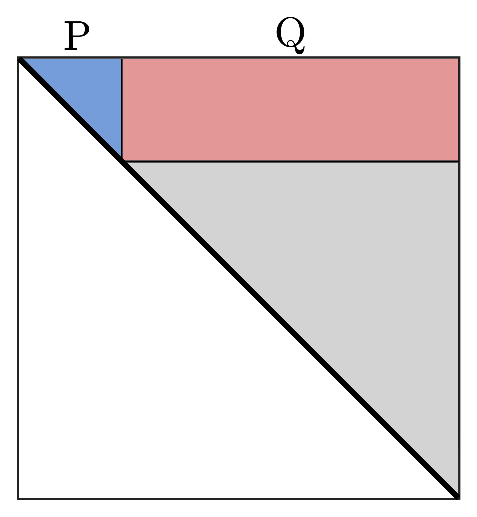
\includegraphics[scale=1]{./figures/CIPT_matrix.eps}
\caption[CIPT matrix structure.]{(First published in Ref. \cite{DBHF2017}). The CIPT matrix structure which is both real and symmetric. The matrix is divided up into three sections for the CIPT calculation. The upper left corner (blue) represents the effective matrix consisting of matrix elements for between states only in set P. The upper middle and right section (red) consists of the matrix elements between states in sets P and Q to be treated perturbatively. The remaining off-diagonal grey matrix elements between states only in set Q are discarded. \label{fig:CIPT_matrix}}
\end{figure}
\iffalse
\subsection{Fast configuration interaction method}
The fast configuration interaction method (FCI) is a more efficient version of the CIPT. It was originally developed in Ref. \cite{FCI} where it was shown to improve the efficiency of the CIPT calculation of the spectrum of Yb by 20 times with a small cost in accuracy ($\approx 200$~cm$^{-1}$). For atoms with open $f$ shells this is important as the CIPT method can still take a significant amount of time to calculate the energy levels. The FCI method is similar to the CIPT method except the PT modification of the CI matrix elements (second term of equation (\ref{eq:HCI})). This term, which takes the most computing time in the CIPT method, is simplied fied by separating out radial and angular integrals of the wavefunction. For some excited configuration $c$, ignoring the differences in energy between the states of the same configuration the second PT modification can be approximated as,
\begin{align}
\sum_k \frac{\langle i|H^{\rm CI}|k\rangle\langle k|H^{\rm
    CI}|j\rangle}{E - E_k} \approx \sum_{c}\dfrac{1}{E - E_c}\sum_{k_c}\langle i|H^{\rm CI}|k_c\rangle\langle k_c|H^{\rm
    CI}|j\rangle.
\end{align}
\fi
\section{Estimation of the accuracy} \label{sec:Accuracy}

Theoretical uncertainty is dominated by incomplete treatment of inter-electron correlations. These correlations can be further separated into core-valence and valence-valence correlations. We will discuss each of these separately. For the SHE calculations, the core includes all states in closed shells
from $1s$ to $5f$ containing one hundred electrons occupying one hundred states.
All other states, including states of the $6d$ and $7s$ shells are treated as
valence states. As mentioned in Section \ref{sec:HF}, using the $V^{N-1}$ HF approximation for an atom with many electrons above a closed shell restricts us from including core-valence correlations and therefore only valence states are used in calculation of the CI matrix.
This means that we neglect core-valence correlations. To estimate the corresponding uncertainties, we perform calculations of the energy levels of gold and roentgenium (Rg, $Z$=111). Both these elements have one external electron above a closed $5d$ or $6d$ shell. We perform the calculations using the correlation potential method~\cite{Dzuba1988, DFSS1987_2}. In this method, core-valence correlation corrections are obtained using the electron self-energy operator (correlation potential) $\Sigma$ is calculated by summation of the diagrams in the many-body perturbation theory. Do not confuse this with  the QED self-energy operator which we included using the radiative potential method \cite{FG2005}. This is the many-body self-energy operator, which for example, has been defined in the textbook \cite{LandauStatPhysPart2}. We calculate this operator using a Feynman diagram technique with relativistic Hartree-Fock Green's functions \cite{Dzuba1988}. The operator $\Sigma $ is defined by the correlation correction to the energy of the valence electron on the orbital $n$, $\delta E_n = \langle n | \Sigma | n \rangle$.   For the Au and Rg calculations, the upper complete $d$-shell ($5d$ or $6d$) is attributed to the core, and the correlation interaction of the external electron with the core is described by a correlation potential $\Sigma$.   \\

Calculation of $\Sigma$ involves a summation over all core states from
$1s$ to $5d$ for Au or $6d$ for Rg. This summation is strongly dominated by the upper $d$-shell. E.g., the $5d$ shell gives about 90\% of the correlation correction to the energies of the $6s$ and $6p$ valence states of Au, and more than 80\% of the correlation correction to the energies of the $7s$ and $7p$ valence states of Rg (see Table \ref{tab:CPaccuracy}). This is because of the small energy interval between the energies of
the $5d$ (or $6d$) state and the energies of lowest valence states.  Since correlation correction to the energy of the $s$ and $p$ valence states is about 20\%, the effect of neglecting inner-core contributions to the core-valence correlations is about 1 to 2\% of the energy of valence states.

%This appears in the correlation
%potential method via small energy denominator in the expression for $\Sigma$,
%which is this small energy interval.

\begin{table}
\centering
\caption[Removal energies of one external electron in Au and Rg using different models]{Removal energies (cm$^{-1}$) for states of external electron of
Au and Rg calculated in different approximations. RHF is relativistic
Hartree-Fock, $\Sigma$($nd$) are Brueckner orbital energies calculated with correlation
potential $\Sigma$, in which summation over core states is limited to $5d$ or
$6d$ shell only. $\Sigma$(all) are the energies calculated with full summation over
core states. \label{tab:CPaccuracy}}
\begin{tabular}{l@{\hspace{0.7cm}}r@{\hspace{0.7cm}}r@{\hspace{0.7cm}}r@{\hspace{0.7cm}}r}
\toprule
\toprule
\multicolumn{5}{c}{Au} \\
  &  \centering    RHF &  $\Sigma$($5d$) &    $\Sigma$(all) &   Expt~\cite{NIST_ASD} \\
  \midrule
$6s_{1/2}$ &  60 179 &  75 539  & 77 878 &  74 409 \\
$6p_{1/2}$ &  29 303 & 36 508  & 37 322 & 37 051 \\
$6p_{3/2}$ &  26 664  & 32 314  & 32 785 & 33 324 \\
$6d_{3/2}$  & 11 929  & 12 423  & 12 439 & 12 457 \\
$6d_{5/2}$ &   11 875  & 12 344 &  12 357 & 12 376 \\
\\
\multicolumn{5}{c}{Rg} \\
    &   \centering  RHF  &    $\Sigma$($6d$) &   $\Sigma$(all)  \\
    \midrule
$7s_{1/2}$  & 83 436 & 101 901 & 106 780 \\
$7p_{1/2}$ &  38 006 &  49 996 &  52 269 \\
$7p_{3/2}$ &  26 550 &  33 659 &  34 685 \\
$7d_{3/2}$  & 11 859 &  12 594 &  12 656 \\
$7d_{5/2}$  & 11 738  & 12 383  & 12 428 \\
\bottomrule
\bottomrule
\end{tabular}
\end{table}

   It is interesting to note that in the second order of many-body perturbation theory, the correlation potential$\Sigma$ always overestimates the value of the correlation correction. This is because it does not include the effect of screening of inter-electron interaction by other atomic electrons. This effect appears in higher orders of perturbation theory. Its proper inclusion leads to very accurate results (see, e.g.~\cite{Dzuba1988, Dzuba2008}).
   
In the CIPT method we have the fortunate situation where neglecting inner-core contributions to $\Sigma$ has a similar affect on its value as the screening would do. In other words, the effect of neglecting the higher-order perturbative contributions on
the calculated energies partially compensates the effect of neglecting
screening of interelectron interactions. The data in Table \ref{tab:CPaccuracy} show that this is the case at least for the
$6s$ state of Au (and probably for the $7s$ state of Rg) where the correlation correction
is the largest in value. Therefore, it is reasonable to assume that the theoretical uncertainty is dominated by valence-valence correlations. The main source for it is the perturbative treatment of the excited configurations. The best way of estimating the uncertainty is to compare the theoretical and experimental energies for lighter elements. This was done in detail for tungsten in the seminal CIPT work~\cite{DBHF2017}, which is the lighter analog of Sg.  This comparison between SHE and lighter analogs was also done for pairs Ta and Db~\cite{LDFDb2018} (covered in Section \ref{sec:TaCIPT} and Chapter \ref{chap:Db}), and Rn and Og~\cite{LDFOg2018} (see Chapter \ref{chap:Og}). As follows from this comparison and from the analysis in Sections \ref{sec:Sg}, \ref{sec:Bh}, the theoretical uncertainty for the energies is on the level of $\sim$ 1000~cm$^{-1}$, sometimes a little higher (e.g.  $\sim$ 2000~cm$^{-1}$ for odd states of Bh). The uncertainty for ionization potentials is on the level of a few percent (see section \ref{sec:SHEIP}).

\section{Example CIPT calculations in Ta and comparison to experiment} \label{sec:TaCIPT}
To demonstrate the accuracy of the CIPT method we compare the theoretical and experimental spectra of Ta~I. The electron states of neutral Ta have an open $5d$ shell, with a  ground state configuration is [Xe]$4f^{14}5d^3 6s^2$. As the $6s$ electrons are easily excited, we should treat the atom as a system with five external electrons. As outlined in Section \ref{sec:HF} we generated the single-electron wavefunctions by removing a $6s$ electron and performing the $V^{N-1}$ HF method with with the electron in the field of the charge core $4f^{14}5d^3 6s$.\\
\linebreak
For every even parity state with angular momentum $J$ we populate the CI matrix with the basis states of the $5d^3 6s^2$, $5d^4 6s$ and $5d^5$  configurations in the effective CI matrix. All other configurations, which were obtained by exciting one or two electrons from these configurations, were included perturbatively. Similarly for the odd parity states (for all angular momenta $J$) we used the states of the $5d^3 6s 6p$, $5d^2 6s^2 6p$ and $5d^4 6p$ configurations in the effective CI matrix, while other configurations are included perturbatively.\\
\linebreak
In Table \ref{tab:TaComparison} we present the comparison between experimental excitation energies and $g$-factors and those calculated by the CIPT method.  We present a significant number of odd parity states to demonstrate the accuracy of these states particularly towards the end of the optical region. This is because the most promising measurements are strong optical electric dipole (E1) transitions between the ground state and excited states of different parity. 
It is important to include as many of these transitions as possible. To identify the correct states for comparison with experiment 
we use the experimental and theoretical Land\'{e} $g$-factors. When experimental $g$-factors were not available we used the next sequential state in the theoretical calculations. There was excellent agreement between the experimental and CIPT $g$-factors with maximum difference between theory and experiment $\Delta g \approx 0.1$. This is sufficient accuracy for identification of the states.\\
%the only significant difference for the odd state $J=1/2$ at $18 505$ cm$^{-1}$.  
\linebreak
From Table \ref{tab:TaComparison} we can see there is good agreement between the experimental and theoretical excitation energies particularly for the low-lying odd parity 
states which are important for measuring the electric dipole transitions (see Section \ref{sec:E1transitions}). For the odd parity
states the largest discrepancy in energy was $\Delta = 453$ cm$^{-1}$ with most states having $|\Delta| \approx 100-400$ 
cm$^{-1}$. The main source of the difference between theory and experiment is incomplete treatment of the correlations by neglecting core-valence correlations and off-diagonal matrix elements between
highly excited states. This is the price we have to pay to be able to perform the calculations for a
complicated system with five external electrons. There are some smaller factors, like cutting basis at $l_{max}=4$, 
ignoring triple excitations, etc.
\afterpage{%
\begin{longtable}{cllcrrrrr}
\caption[Comparison of experimental and CIPT spectra and ionisation potential of Ta~I]{Comparison of experimental (from ref.\cite{NIST_ASD}) and CIPT spectra and ionisation potential of Ta I. The experimental excitation energies ($E_E$) and Land\'{e} g-factors ($g_E$) are compared to respective CIPT excitation energies ($E_T$) and Land\'{e} g-factors ($g_T$).   The final column is the difference between experimental and theoretical excitation energies $\Delta = E_{E} - E_{T}$. \textit{The results of this table was published in Ref. \cite{LDFDb2018}} \label{tab:TaComparison}}\\
\endfirsthead
\multicolumn{5}{c}%
{\tablename\ \thetable\ -- \textit{Continued from previous page}} \\
\hline
&  & & \multicolumn{2}{c}{Experimental} & \multicolumn{2}{c}{CIPT} &  \\
\cmidrule{4-5} \cmidrule{6-7}
& Configuration & State  &  \multicolumn{1}{c}{\parbox{1cm}{ $E_E$ \\ (cm$^{-1}$)}}  &  \multicolumn{1}{c}{$g_E$} &  \multicolumn{1}{c}{\parbox{1cm}{$E_T$ \\ (cm$^{-1}$)} } &  \multicolumn{1}{c}{$g_T$} &  \multicolumn{1}{c}{\parbox{1cm}{$\Delta$ (cm$^{-1}$)} } \\
\hline
\endhead
\hline \multicolumn{5}{r}{\textit{Continued on next page}} \\
\endfoot
\endlastfoot
\toprule
\toprule
&  & & \multicolumn{2}{c}{Experimental} & \multicolumn{2}{c}{CIPT} &  \\
\cmidrule{5-6} \cmidrule{7-8}
& Configuration & State  &  \multicolumn{1}{c}{\parbox{1cm}{ $E_E$ \\ (cm$^{-1}$)}}  &  \multicolumn{1}{c}{$g_E$} &  \multicolumn{1}{c}{\parbox{1cm}{$E_T$ \\ (cm$^{-1}$)} } &  \multicolumn{1}{c}{$g_T$} &  \multicolumn{1}{c}{\parbox{1cm}{$\Delta$ (cm$^{-1}$)} } \\
\midrule
\multicolumn{5}{r}{ Even states}\\
(1)  &$5d^3 6s^2$ & $^4$F$_{3/2}$   & 0.00 & 0.447 &  0.00 & 0.4373 & \\
(2)  &$5d^3 6s^2$ & $^4$F$_{5/2}$   & 2 010 & 1.031 &  1 652 & 1.0336 & 358 \\
(3)  &$5d^3 6s^2$ & $^4$F$_{7/2}$   & 3 964 & 1.218 & 3 175 & 1.2265 &  789\\
(4)  &$5d^3 6s^2$ & $^4$F$_{9/2 }$  & 5 621 & 1.272 & 4 679 & 1.3066 & 942\\
(5)  &$5d^3 6s^2$ & $^4$P$_{1/2}$  & 6 049 & 2.454 & 6 017 & 2.4022 & 32\\
\\
\multicolumn{5}{r}{ Odd states}\\
(6)  &$5d^3 6s 6p$ & $^6$G$^{\rm_o}_{3/2}$    & 17 385 &  & 17 599 &   0.1719   &  -214\\
(7)  &$5d^3 6s 6p$ & $^2$F$^{\rm_o}_{5/2}$    & 17 994 & 0.732 &  18 225 &   0.7955  & -231\\
(8)  &$5d^2 6s^2 6p$ & $^4$D$^{\rm_o}_{1/2}$    & 18 505 & 0.172 & 18 629 &   0.0716  & -124\\
(9)  &$5d^3 6s 6p$ & $^6$G$^{\rm_o}_{5/2}$    & 19 178 & 0.851 & 19 393 &   0.8551 &  -123\\
(10)  &$5d^2 6s^2 6p$ & $^4$D$^{\rm_o}_{3/2}$    & 19 658 & 1.018 & 19 724 &   0.9389 & -66\\
(11)  &$5d^2 6s^2 6p$ & $^2$S$^{\rm_o}_{1/2}$    & 20 340 & 1.956 & 20 574 &   2.0278 & -233\\
(12)  &$5d^3 6s 6p$ & $^6$G$^{\rm_o}_{7/2}$    & 20 560 & 1.194 & 20 463 &   1.1394 & -97\\
(13)  &$5d^2 6s^2 6p$ & $^2$D$^{\rm_o}_{3/2}$    & 20 772 & 0.812 & 20 796 &     0.8124 & -24\\
(14)  &$5d^2 6s^2 6p$ & $^4$D$^{\rm_o}_{5/2}$    & 21 168 &   & 21 358 &   1.2117 &  -190\\
(15)  &$5d^3 6s 6p$ & $^4$F$^{\rm_o}_{3/2}$   & 21 855 & 0.666 & 22 132 & 0.6773 & -277 \\
(16)  &$5d^2 6s^2 6p$ & $^2$D$^{\rm_o}_{5/2}$  & 22 047 & 1.179 & 21 875 & 1.0838 & 172 \\
(17)  &$5d^2 6s^2 6p$ & $^4$G$^{\rm_o}_{7/2}$    & 22 381 & 1.060 & 22 276 & 1.0377 & 105 \\
(18)  &$5d^3 6s 6p$ & $^6$G$^{\rm_o}_{9/2}$   & 22 682 & 1.231 & 22 285 & 1.2677 & 397 \\
(19)  &$5d^3 6s 6p$ & $^6$F$^{\rm_o}_{1/2}$  & 23 355 & -0.320 & 23 680 & -0.2689 & -325 \\
(20)  &$5d^3 6s 6p$ & $^4$F$^{\rm_o}_{5/2}$   & 23 363 & 1.078 & 23 381 & 1.0766 & -18 \\
(21)  &$5d^2 6s^2 6p$ & $^4$D$^{\rm_o}_{7/2}$   & 23 927 & 1.326 & 23572 & 1.3256 & 355 \\
(22)  &$5d^3 6s 6p$ & $^6$F$^{\rm_o}_{3/2}$   & 24 243 & 1.126 & 24 463 & 1.1018 & -220 \\
(23)  &$5d^3 6s 6p$ & $^6$D$^{\rm_o}_{1/2}$   & 24 517 & 2.888 & 24 907 & 2.9261 & -390 \\
(24)  &$5d^3 6s 6p$ & $^6$D$^{\rm_o}_{3/2}$   & 24 739 & 1.620 & 25 143 & 1.6808& -404 \\
(25)  &$5d^3 6s 6p$ & $^4$F$^{\rm_o}_{7/2}$    & 24 982 & 1.235  & 24 922 & 1.2590 & 60 \\
(26)  &$5d^3 6s 6p$ & $^6$G$^{\rm_o}_{11/2}$ & 25 009 & 1.302 & 24 528 & 1.3366 & 481 \\
(27)  &$5d^3 6s 6p$ & $^6$F$^{\rm_o}_{5/2}$ &   25 181 & 1.239 & 25 267 & 1.2573 & -86 \\
(28)  &$5d^3 6s 6p$ & $^6$G$^{\rm_o}_{9/2}$ &   25 186 &  & 24 733  & 1.2540 & 453 \\
(29)  &$5d^3 6s 6p$ & $^4$D$^{\rm_o}_{1/2}$ &   25 513 & 0.028 & 25 697 & 0.0319  & -184 \\
(30)  &$5d^3 6s 6p$ & $^4$F$^{\rm_o}_{9/2}$  &   25 926 &  1.292 & 25 509 & 1.2970 & 417 \\
(31)  &$5d^2 6s^2 6p$ & $^4$P$^{\rm_o}_{5/2}$ &  26 220 & 1.338 & 26 298 & 1.2923 & -78 \\
(32)  &$5d^3 6s 6p$ & $^4$D$^{\rm_o}_{3/2}$ &   26 364 & 1.393 & 26 678 & 1.2676 & -314 \\
(33)  &$5d^3 6s 6p$ & $^6$F$^{\rm_o}_{7/2}$  &  26 586 & 1.356  & 26 299 & 1.315 & 287 \\
(34)  &$5d^2 6s^2 6p$ & $^4$P$^{\rm_o}_{3/2}$   & 26 590 & 1.576 & 26 759 & 1.6833 & -169\\
(35)  &$5d^3 6s 6p$ & $^6$D$^{\rm_o}_{5/2}$ &   26 795 & 1.416 & 26 815 & 1.4086 & -20 \\
(36)  &$5d^2 6s^2 6p$ & $^4$P$^{\rm_o}_{1/2}$ &   26 866 & 2.650 & 27 094 & 2.6189 & -228\\
(37)  &$5d^3 6s 6p$ &  $^4$F$^{\rm_o}_{7/2}$   &   26 960 & 1.223  & 26 787 & 1.2390 & 173 \\
(38)  &$5d^3 6s 6p$ & $^6$F$^{\rm_o}_{9/2}$  &   27 733 &  1.390 & 27 279 & 1.3590 & 454 \\
(39)  &$5d^3 6s 6p$ & $4$D$^{\rm_o}_{7/2}$   &   27 781 & 1.374  & 27 643 & 1.4658 & 138 \\
(40)  &$5d^3 6s 6p$ & $^6$G$^{\rm_o}_{11/2}$ &   27 783 & 1.351 &  27 376 & 1.350  & 407\\
(41)  &$5d^3 6s 6p$ & $^4$D$^{\rm_o}_{5/2}$ &   28 134 & 1.394 & 28 337 & 1.3665 & -203 \\
(42)  &$5d^3 6s 6p$ & $^4$G$^{\rm_o}_{7/2}$   &   28 183 & 1.115  & 27 970 & 1.0421 & 213 \\
(43) &$5d^3 6s 6p$ & $^2$P$^{\rm_o}_{3/2}$   &   28 689 & 1.356  & 28 693 & 1.3052  & -4 \\
(44)  &$5d^3 6s 6p$ & $^6$D$^{\rm_o}_{9/2}$  &   28 767 &  1.337 & 28 414 & 1.4106 & 353 \\
(45)  &$5d^3 6s 6p$ & $^6$F$^{\rm_o}_{5/2}$ &   28 862 & 1.247 & 28 868 & 1.2678 & -6 \\
(46)  &$5d^3 6s 6p$ & $^6$D$^{\rm_o}_{1/2}$ &   29 902 & 2.994 & 30 323 & 2.9971 & -421 \\
\\
\multicolumn{5}{r}{ Ta I ionisation potential} \\
(47)  &$5d^3 6s$& $5$F$_1$  & 60 891 & 0.000 & 61 073 &    0.0235 &  -182\\
\bottomrule
\bottomrule
\end{longtable}
}
In Table \ref{tab:TaComparison} we present the comparison between experimental excitation energies and $g$-factors and those calculated by the CIPT method.  We present a significant number of odd parity states to demonstrate the accuracy these states particularly towards the end of the optical region. This is because the most promising measurements are strong optical electric dipole (E1) transitions between the ground state and excited states of different parity. 
It is important to include as many of these transitions as possible. To identify the correct states for comparison with experiment 
we use the experimental and theoretical Land\'{e} $g$-factors. When experimental $g$-factors were not available we used the next sequential state in the theoretical calculations. There was excellent agreement between the experimental and CIPT $g$-factors with maximum difference between theory and experiment $\Delta g \approx 0.1$. This is sufficient accuracy for identification of the states.
%the only significant difference for the odd state $J=1/2$ at $18 505$ cm$^{-1}$.  

There is good agreement between the experimental and theoretical excitation energies particularly for the low-lying odd parity 
states which are important for measuring the electric dipole transitions (see Section \ref{sec:E1transitions}). For the odd parity
states the largest discrepancy in energy was $\Delta = 453$ cm$^{-1}$ with most states having $|\Delta| \approx 100-400$ 
cm$^{-1}$. The main source of the difference between theory and experiment is incomplete treatment of the correlations,
which mostly comes from two factors. We neglect core valence correlations and off-diagonal matrix elements between
highly excited states. This is the price we have to pay to be able to perform the calculations for a
complicated system with five external electrons. There are some smaller factors, like cutting basis at $l_{max}=4$, 
ignoring triple excitations, etc.
%Our calculations also supported the existence of the $J=11/2$ level at $E_E=  27 783$ cm$^{-1}$ which is listed as ambiguous \cite{NIST_ASD}.  
For the CIPT calculations of the Db I spectrum we expect a similar accuracy as seen in Ta~I due to the similar electronic structure.\\

\chapter{Atomic structure of super heavy element Db } \label{chap:Db}
The super heavy element (SHE) dubnium ($Z=105$), was first officially synthesized in 1970 with recognition of its discovery being shared between the Joint Institute for Nuclear Research and the Lawrence Berkeley Laboratory after much disagreement over the validity of initial discovery claims \cite{Barber1992}.  Currently, the longest living isotope is $^{268}$Db with a half-life of approximately $ 30 $ hrs \cite{Schadel2012, Oganessian2005}. This lifetime  is anomalous among the known SHE isotopes which have half-lives of at most minutes or seconds. This relatively large half-life is promising for future experiments as it is typically the short lifetimes (along with the low production rates) which make SHE experiments difficult. There is limited experimental and theoretical data for Db with the majority being chemical properties~\cite{Schadel2012, Fricke1975} with recent theoretical work (after the publication of our results) on the low lying spectrum using CIPT+MBPT method \cite{Geddes2018}.  An estimation of the ionisation potential has been performed for Db in Ref.~\cite{Dzuba2016} using a relativistic 
 Hartree-Fock  method with semi-empirical corrections introduced to simulate the effect of correlations. The results of this chapter were published in Ref. \cite{LDFDb2018}.
\section{Calculation of Excitation spectrum}
For the CIPT calculations of Db~I we use the same parameters as for the Ta~I calculations in Section \ref{sec:TaCIPT}. As Db is the SHE analog of Ta, we expect that by using an identical method with only the electronic configurations changed ($5d \rightarrow 6d$ and $6s \rightarrow 7s$) the accuracy of the results should be similar. In the $V^{N-1}$ approximation discussed in Section \ref{sec:CIPT} we remove a $7s$ electron in the initial Hartree-Fock calculations and in the calculation of the single-electron basis states. The Db~I ground state is [Rn]$5f^{14}6d^3 7s^2$ which is similar to Ta I with different principle quantum numbers. For calculation of the even parity states we populated the effective CI matrix with the states of the $6d^3 7s^2$,  $6d^4 7s$ and $6d^5$ configurations. All higher states are obtained through single and double excitations of these states and are included perturbatively. Similarly for  the states of odd parity the effective matrix contains states of the  $6d^3 7s 7p$, $6d^2 7s^2 7p$ and $6d^4 7p$ configurations. Other configurations are included perturbatively. For the ion  we use the states of the $6d^3 7s$, $6d^2 7s^2$ and $6d^4$ configurations.  Both Breit and radiative corrections are expected to be larger in SHE compared to lighter elements and therefore are included in Table~\ref{table:DbISpectrum}. In Table~\ref{table:DbISpectrum} we present the excitation energies of Db using the CIPT method. To demonstrate the affect of  Breit and QED corrections we performed four separate calculations,
first with no Breit or QED corrections ($E_{NC}$), second with only Breit correction included ($\Delta_{B}$), then with QED included but no Breit ($\Delta_{R}$), and finally,
with both corrections included ($E_T$) (see Table~\ref{table:DbISpectrum}).\\
\linebreak
\afterpage{
\begin{longtable}{cllrrrrr}
\caption[Low lying energy spectrum of Db I and Db II calculated using the CIPT method]{Spectrum for the low lying energy levels of Db I and Db II using the CIPT method. Here $E_{NC}$ are the excitation energies when neither Breit nor radiative corrections are included in the calculations, $\Delta_B$ and $\Delta_R$ are the changes in energy from $E_{NC}$ when Breit and radiative corrections are included respectively. The final energy $E_T$ is the excitation spectrum when both Breit and radiative corrections are included \textit{ab initio}. The accuracy of these levels is expected to be similar to Ta I presented in Table \ref{tab:TaComparison}. (Originally published in \cite{LDFDb2018}). \label{table:DbISpectrum}} \\
\endfirsthead
\multicolumn{5}{c}%
{\tablename\ \thetable\ -- \textit{Continued from previous page}} \\
\hline
  & &  & \multicolumn{4}{c}{Excitation energy (cm$^{-1}$)} &\\
  \cmidrule{4-7}
& Configuration & State & $E_{NC}$  &  $\Delta_B$  & $\Delta_R$ &  $E_T$  & Land\'{e} g-factor \\ 
\hline
\endhead
\hline \multicolumn{5}{r}{\textit{Continued on next page}} \\
\endfoot
\endlastfoot
\toprule
\toprule
  & &  & \multicolumn{4}{c}{Excitation energy (cm$^{-1}$)} &\\
  \cmidrule{4-7}
& Configuration & State & $E_{NC}$  &  $\Delta_B$  & $\Delta_R$ &  $E_T$  & Land\'{e} g-factor \\ 
\midrule
& \multicolumn{5}{l}{Even States}  \\
(1)  &   $6d^3 7s^2$  &  $^4$F$_{3/2}$  &   0 & 0 & 0 & 0 & 0.554 \\ 
(2) &   $6d^3 7s^2$  &  $^4$F$_{5/2}$   &  4 072 & -77 & 21 & 4 016 & 1.043 \\ 
(3)  &  $6d^3 7s^2$  &  $^2$F$_{7/2}$   &  6 595 & -100 & 31 & 6 527 & 1.170 \\ 
(4)  &  $6d^3 7s^2$  &  $^2$S$_{1/2}$   &  7 691 &  -73  &  16 & 7 634 & 2.058 \\ 
(5)  &  $6d^3 7s^2$  &  $^4$G$_{9/2}$ &    8 076 & -92 &  33 & 8 017 & 1.191 \\ 
& \multicolumn{5}{l}{Odd States}  \\
(6) & $6d^2 7s^2 7p$  &  $^2$F$^{\rm_o}_{5/2}$  &   6 255 & 213 &  123 & 6 591 & 0.739 \\ 
(7)  & $6d^2 7s^2 7p$  &  $^2$D$^{\rm_o}_{3/2}$  &   11 240 & 156 &  87 & 11 483 &  0.633 \\ 
(8)  &   $6d^2 7s^2 7p$  &  $^2$P$^{\rm_o}_{1/2}$ &    12 642 & 140 &  84  & 12 869 & 1.308 \\ 
(9)  &  $6d^2 7s^2 7p$  &  $^4$G$^{\rm_o}_{7/2}$ &    13 645 &  116 &  147 & 13 909 & 1.023 \\ 
(10)   &  $6d^2 7s^2 7p$  &  $^4$F$^{\rm_o}_{5/2}$  &   13 873 & 113  &  132 & 14 117 & 1.067 \\ 
(11)   &  $6d^2 7s^2 7p$  &  $^2$P$^{\rm_o}_{1/2}$  &   14 516 & 96  &  88  & 14 705 & 0.995 \\ 
(12)   &  $6d^2 7s^2 7p$  &  $^6$F$^{\rm_o}_{3/2}$  &   14 572 & 105 & 96  & 14 772 & 1.111 \\ 
(13)   &  $6d^2 7s^2 7p$  &  $^4$F$^{\rm_o}_{5/2}$ &    17 493 & 78 &76  & 17 647 & 1.111 \\ 
(14)  &  $6d^2 7s^2 7p$  &  $^4$G$^{\rm_o}_{9/2}$   &  18 596 & 80 &  144  & 18 820  & 1.145 \\ 
(15)  & $6d^3 7s 7p$  &  $^2$D$^{\rm_o}_{3/2}$  &  19 379 & 62 &  -3  & 19 438 & 0.701 \\ 
 (16)  &  $6d^2 7s^2 7p$  &  $^4$F$^{\rm_o}_{7/2}$ &    20 462 & 53 & 134 & 20 649  & 1.203 \\ 
(17)  &  $6d^2 7s^2 7p$  &  $^6$F$^{\rm_o}_{3/2}$  &   21 706 & 56  & 50 & 21 811 & 1.073 \\ 
(18)  &  $6d^2 7s^2 7p$  &  $^4$D$^{\rm_o}_{1/2}$ &    22 123 & 72  & 93 & 22 284 & 0.078 \\ 
(19)   &  $6d^2 7s^2 7p$  &  $^4$F$^{\rm_o}_{5/2}$ &    22 204 & 35  & 54 & 22 292 & 1.110 \\ 
(20)  &  $6d^2 7s^2 7p$  &  $^2$D$^{\rm_o}_{3/2}$  &   23 003 & 39 & 22 & 23 067 & 0.697 \\ 
(21)  &  $6d^2 7s^2 7p$  &  $^2$F$^{\rm_o}_{7/2}$ &    23 221 & 37   & 133 & 23 390 & 1.102 \\ 
(22)  &  $6d^3 7s 7p$  &  $^4$F$^{\rm_o}_{5/2}$  &   23 910 &  4 &  -2 & 23 913 & 0.948 \\ 
(23) &   $6d^2 7s^2 7p$  &  $^2$P$^{\rm_o}_{3/2}$ &    24 622 & 2  &  119  & 24 743  & 1.372 \\ 
(24)  &   $6d^2 7s^2 7p$  &  $^2$G$^{\rm_o}_{9/2}$  &  24 915&  27  & 133 & 25 074 & 1.111 \\ 
 (25)  & $6d^3 7s 7p$  &  $^2$F$^{\rm_o}_{7/2}$ &    25 458 & 9  & 17  & 25 480 & 1.152 \\ 
(26) &   $6d^2 7s^2 7p$  &  $^4$F$^{\rm_o}_{5/2}$ &    25 510 & 5   & 73 & 25 589 & 1.031 \\ 
(27)   & $6d^2 7s^2 7p$  &  $^2$F$^{\rm_o}_{7/2}$ &    26 538 & -4   &  78 & 26 612 & 1.172 \\ 
(28)   &  $6d^2 7s^2 7p$  &  $^2$S$^{\rm_o}_{1/2}$ &    27 435 & -10   &  49 & 27 479 & 1.663 \\ 
(29)  &   $6d^2 7s^2 7p$  &  $^2$F$^{\rm_o}_{7/2}$ &    27 662 & -23   & 24  & 27 666 & 1.128  \\ 
(30)  &  $6d^2 7s^2 7p$  &  $^4$D$^{\rm_o}_{3/2}$ &    27 589 & -5   & 114 & 27 697  & 1.147 \\ 
(31)  &  $6d^2 7s^2 7p$  &  $^4$G$^{\rm_o}_{9/2}$ &    27 885 & -13   &  118 & 27 990 & 1.173 \\ 
(32)   & $6d^2 7s^2 7p$  &  $^2$D$^{\rm_o}_{5/2}$ &    28 162 & -25  & 75 & 28 211  & 1.130 \\ 
(33)    &  $6d^2 7s^2 7p$  &  $^4$P$^{\rm_o}_{3/2}$ &    29 183 & 1  & 74 & 29 259 & 1.659 \\ 
(34)  & $6d^2 7s^2 7p$  &  $^4$G$^{\rm_o}_{11/2}$ &    29 669 & -45 & 103 & 29 669 & 1.254 \\ 
(35)  & $6d^3 7s 7p$  &  $^6$G$^{\rm_o}_{9/2}$ &    29 946 & -75  & -87 & 29 784 & 1.254 \\ 
(36)  &   $6d^2 7s^2 7p$  &  $^6$F$^{\rm_o}_{5/2}$   &  29 734 &  -25  & 174  & 29 821 & 1.343 \\ 
(37) &  $6d^3 7s 7p$  &  $^4$D$^{\rm_o}_{1/2}$  &  29 886 & -24  &  -33  & 29 832 & 0.220 \\ 
(38)  &  $6d^2 7s^2 7p$  &  $^2$F$^{\rm_o}_{7/2}$   &  30 474 & -29  & 97 & 30 541  & 1.161 \\ 
 & \multicolumn{5}{l}{Db II states} \\
(39)  &   $6d^2 7s^2$  &  $^3$F$_2$  & 56 546 & 48 & 139 & 56 733 & 0.731 \\ 
(40)  &   $6d^2 7s^2$  &  $^3$S$_0$  & 62 673 & -13 & 119 & 62 778 & 0.000 \\ 
(41)  &   $6d^2 7s^2$  &  $^3$F$_3$ & 62 952 & -45 & 176 & 63 083 & 1.083 \\ 
(42)  &   $6d^2 7s^2$  &  $^3$D$_2$  & 65 122 & -62 & 120 & 65 179 & 1.250 \\ 
(43)  &   $6d^2 7s^2$  &  $^3$P$_1$  & 65 587 & -79 & 113 & 65 620 & 1.467 \\ 
(44)  &   $6d^2 7s^2$  &  $^5$G$_4$  & 67 466 & -83 & 189 & 67 572 & 1.120 \\ 
\bottomrule 
 \bottomrule 
\end{longtable} 
%\end{adjustwidth}
%\end{table*}
}

Comparing the Db~I spectrum in Table~\ref{table:DbISpectrum} to the Ta~I spectrum in Table~\ref{tab:TaComparison} we see there are some notable differences. While the order of even parity states has remained the same relative to each other,  the order of the odd states has been significantly altered with the first $2F^{\rm_o}_{5/2}$ state being significantly lowered in the spectrum. Another thing to note is that the odd parity excitations are typically $6d \rightarrow 7p$ as opposed to the Ta excitation $6s \rightarrow 6p$. This can be explained by relativistic effects where the $7s$ electrons are more tightly bound than the $6d$ electrons in contrast to the $5d$ and $6s$ electrons in Ta \cite{Schwerdtfeger2014}. These relativistic effects also cause the $6d$ electron to be ionised in Db instead of the $7s$ electron. This may result in significantly different chemical properties in Db compared to Ta. \\
\linebreak
To understand the difference between the atoms it is instructive to look at the Hartree-Fock energies and electron 
densities calculated in non-relativistic and relativistic approximations. Fig.~\ref{f:el} shows energies of the upper
core states of Ta and Db. The spectra are very similar. Relativistic energy shifts are larger for Db as expected and
the most noticeable difference cause by this shift is the change of the order of the $6d$ and $7s$ states which leads 
to the  change of the dominant configurations in low odd states of Db as discussed above.  However, the absolute
shift of the energies is small. It changes the order of the states because they are very close in the non-relativistic
calculations. This change in the Hartree-Fock spectra caused by relativistic effects suggests that the differences 
in the spectra of neutral Ta and Db are mostly due to relativistic effects while correlation corrections are
similar. This means that the accuracy of the calculations should also be similar for Ta and Db.
This can be further illustrated by comparing the electron densities of the atoms calculated in non-relativistic and relativistic
approximations (see Fig.~\ref{f:ro}). Examining the densities one can see the following:
\begin{enumerate}
\item There are four peaks for Ta and five for Db. They correspond to shells with principal quantum numbers from 1 to 4 for
Ta and 1 to 5 for Db. Electrons in higher shells are distributed over larger distances and their density does not form a peak.
\item   Relativistic effects pull inner electrons towards the nucleus but have little effect on outer electrons.
\item The densities at large distances ($r>a_B$), where external electrons are located, are very similar.
\end{enumerate}
This is another indication that correlations are likely to be similar.  To check this we performed another test. We
compared the contribution of high energy states (second term in (\ref{eq:HCI})) to the energies of Ta and Db.
It turns out that the corrections to the energies of even states of Ta and Db differ by 2\% only while corrections to 
the energies of odd states of Db about 30\% larger than those of Ta. This means the uncertainty in the calculations for these
states might also be larger for Db. Therefore, it seems to be reasonable to increase estimated uncertainty from 
$ \sim 400$~cm$^{-1}$ for Ta to $ \sim 500$~cm$^{-1}$ for Db.
\begin{figure}[tb]
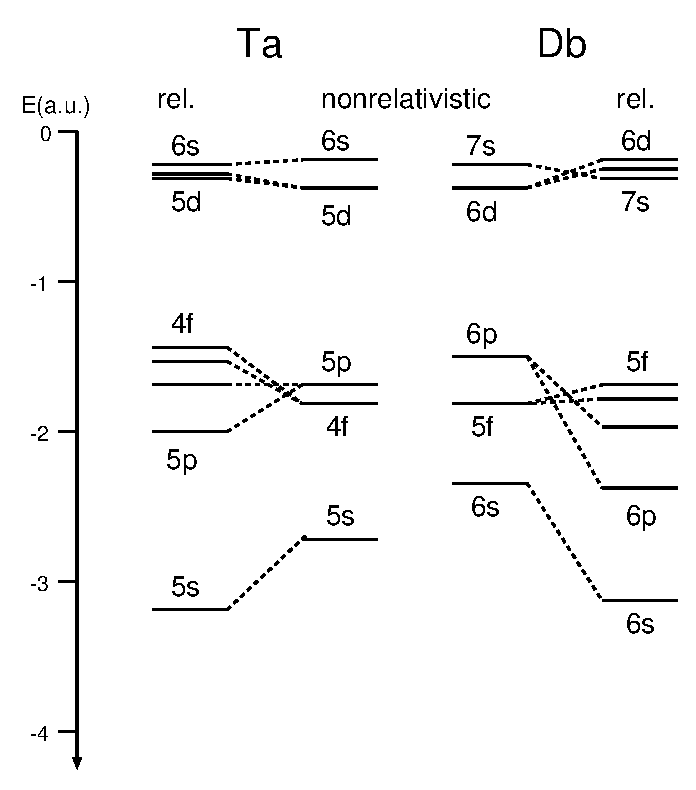
\includegraphics[scale=0.7]{./figures/el.eps}
\caption{Hartree-Fock energies of upper core states of Ta and Db calculated in non-relativistic and relativistic 
approximations.}
\label{f:el}
\end{figure}
\begin{figure}[tb]
\includegraphics[scale=0.45]{./figures/ro.eps}
\caption[Relativistic and non-relativistic  electron densities of Db and Ta.]{Electron density normalized to one ($\int \rho dV = 1$) of Db and Ta  calculated in non-relativistic (solid line)
and relativistic (dotted line) approximations.}
\label{f:ro}
\end{figure}
From Table~\ref{table:DbISpectrum} we see that the effect of both the Breit interaction ($\Delta_B$) and radiative corrections 
($\Delta_R$)  is small and lies within the accuracy of our CIPT method. As it was discussed in previous section the main
source of the uncertainty of the calculations comes from incomplete treatment of the correlations and it is $ < 500$~cm$^{-1}$
for Ta. It is expected to be similar for Db. On the other hand, the maximum value of the sum of Breit and QED corrections for 
Db is $\sim 300$~cm$^{-1}$ while for most of the states it is $< 200$~cm$^{-1}$ (see Table~\ref{table:DbISpectrum}).
It is interesting that the Breit and QED effects do not correlate with each other. This can be seen by summing the two  
corrections and the calculated energy with no  corrections included ($E_{NC}$). This energy is very close to states in 
the spectrum which include both corrections simultaneously,
\begin{align*}
E \approx E_{NC} + \Delta_B + \Delta_R.
\end{align*}
Including both Breit and QED effects simultaneously will introduce new terms which are second order in perturbations of the interactions. Since both corrections are small these new terms will be negligible.
To test the consistency of our method we calculated the spectrum of Db~I using the $V^{N-1}$ approach removing a $6d$ electron for the frozen core potential. In these calculations we obtained a similar spectrum within the accuracy of our calculations.\\
\linebreak
During completion of our work another paper on calculation of the Db spectrum appeared~\cite{Geddes2018}.
The calculations are done with a different implementation of a very similar method. The difference between the results 
of two papers seems to be larger than the uncertainty of our calculations. However, if we accept the difference between 
theory and experiment for Ta in~\cite{Geddes2018} as an estimation of the uncertainty of their calculations, the results
are consistent. \\
\linebreak
Comparing our calculations of the IP of Db spectrum with other values in literature we find our value 56744~cm$^{-1}$ is in good agreement with the Hartree-Fock number 55000(7000)~cm$^{-1}$~\cite{Dzuba2016} and
coupled cluster number 55590~cm$^{-1}$~\cite{BorschevskyPC}. Note that the IP of Db is significantly smaller than the IP
of Ta (IP(Ta)=60891~cm$^{-1}$, see previous section) which is another indication of possible different chemical properties. 
\section{Electric dipole transitions and isotope shift} \label{sec:E1transitions}
Due to the current low production rate of dubnium and other SHEs, broad spectroscopic scans are unfeasible for current experimental methods. Therefore experimental searches need to be assisted with theoretical predictions of the strongest lines specifically for optical electric dipole (E1) transitions. In this work we calculate and present the E1 transition amplitudes for the major optical  transitions between the ground state and the  lowest lying odd parity states for each Ta~I and Db~I. It should be noted that there is no published data for the E1 transitions for either Ta~I or Db~I and therefore we present the E1 transition amplitudes ($D_{E1}$)  and transition probabilities ($A_{E1}$) for both atoms. \\
\linebreak
To calculate the E1 transition amplitudes $D_{E1}$ we use the self-consistent random-phase approximation (RPA) to simulate the atom in an external electromagnetic field. This results in an effective electric dipole field for the electrons. The E1 transition amplitude for a transition between states $a$ and $b$ is given by $D_{E1} = \left< b || \hat D + \delta V || a\right>$ where $|a>$ and $|b>$ are the many electron wavefunctions calculated in the CIPT method above, $\hat D$ is the electric dipole operator acting on external electrons, $\delta V$ is the correction to the self-consistent Hartree-Fock potential of atomic core caused by photon electric field. For a more in depth discussion on this method refer to ref. ~\cite{Dzuba2018}. \\
\linebreak
The E1 transition rates are calculated using (in atomic units),
\begin{align*}
A_{E1} = \dfrac{4}{3}\left(\alpha \omega\right)^3\dfrac{ D_{E1}^2}{2J + 1}
\end{align*}
where $J$ is the angular momentum of the odd parity state, $\alpha$ is the fine structure constant and $\omega$ is the frequency of the transitions in atomic units. All calculations obey the selection rules for E1 transitions, a change in parity and change in angular momenta $|\Delta J| \leq 1 $. We present the E1 transitions for Ta I and Db I in Table \ref{table:E1Amplitudes}.\\
\begin{table*}[t!] 
\centering
\caption[Electric dipole amplitudes and rates for allowed transitions in Ta I calculated using the CIPT method]{Allowed electric dipole transitions between the  ground states of Ta I ($^4F_{3/2}$) and its low lying odd parity states.  The numbers next to the states correspond to the numbered spectra in Tables \ref{tab:TaComparison}. The transition amplitudes $D_{E1}$ are in atomic units. (Originally published in \cite{LDFDb2018}) \label{table:E1Amplitudes} }
\begin{tabular}{cl@{\hspace{0.75cm}}r@{\hspace{0.75cm}}r@{\hspace{0.75cm}}}  % @{} adds extra padding to the columns 
\toprule
\toprule
\multicolumn{4}{c}{Ta I}  \\ \\
 & State &   \multicolumn{1}{c}{\parbox{1cm}{$D_{E1}$ \\ (a.u)}} & \parbox{1.5cm}{$A_{E1}$ \\ $(\times 10^{6} \ \text{s}^{-1})$ } \\
\midrule
 (6) & $^6$G$^{\rm_o}_{3/2}$  & -0.270   & 0.194   \\
(7) & $^2$F$^{\rm_o}_{5/2}$  & 0.214 &  0.090   \\
(8) & $^4$D$^{\rm_o}_{1/2}$   & -0.641   & 2.64  \\
 (9) & $^6$G$^{\rm_o}_{5/2}$  & -0.434   & 0.449   \\
 (10) & $^4$D$^{\rm_o}_{3/2}$   & 0.149   &  0.0856   \\
 (11) &$^2$S$^{\rm_o}_{1/2}$    & -0.107  & 0.0973   \\
 (13) &$^2$D$^{\rm_o}_{3/2}$    & 0.495   & 1.12  \\
 (14) &$^4$D$^{\rm_o}_{5/2}$   & -0.200   &  0.128    \\
 (15) &$^4$F$^{\rm_o}_{3/2}$  & -0.360   & 0.688   \\
 (16) &$^2$D$^{\rm_o}_{5/2}$    & 0.069   & 0.0160   \\
 (19) &$^6$F$^{\rm_o}_{1/2}$   &   0.019   & 0.00446  \\
 (20) &$^4$F$^{\rm_o}_{5/2}$   &  -0.094   & 0.0381  \\
 (22) &$^6$F$^{\rm_o}_{3/2}$  & 0.007   & 0.000412  \\
 (23) &$^6$D$^{\rm_o}_{1/2}$    & -0.073   & 0.0795 \\
 (24) &$^6$D$^{\rm_o}_{3/2}$ & -0.249   & 0.477 \\
 (27) &$^6$F$^{\rm_o}_{5/2}$   & -0.356   & 0.683   \\
 (29) &$^4$D$^{\rm_o}_{1/2}$   &  0.282   & 1.34 \\
 (31) &$^4$P$^{\rm_o}_{5/2}$ & 0.202   & 0.248 \\
 (32) &$^4$D$^{\rm_o}_{3/2}$   & 0.405   & 1.53    \\
 (34) &$^4$P$^{\rm_o}_{3/2}$   &  -0.063   & 0.0377 \\
 (35) &$^6$D$^{\rm_o}_{5/2}$  & 0.338   & 0.741   \\
 (36) &$^4$P$^{\rm_o}_{1/2}$    & -0.066   & 0.0859  \\
 (41) &$^6$D$^{\rm_o}_{5/2}$  & -0.278   & 0.583  \\
 (43) & $^2$P$^{\rm_o}_{1/2}$  &  -0.295   & 1.04  \\
\bottomrule
\bottomrule
\end{tabular}
\end{table*}

\begin{table*}[t!] 
\centering
\caption[Electric dipole amplitudes, rates and associated isotope shifts in Db I calculated using the CIPT method]{Allowed electric dipole transitions and associated isotope shift parameters $a$ and $F$  between the  ground state of Db I ($^4F_{3/2}$) and its low lying odd parity states.  The numbers next to the states correspond to the numbered spectra in Table \ref{table:DbISpectrum}. The transition amplitudes $D_{E1}$ are in atomic units. The isotope shift calculation was performed for $^{268}$Db ($\left<r^{2}\right>_{268} = 36.770$ fm$^2$) and $^{289}$Db ($\left<r^{2}\right>_{289}=38.470$ fm$^2$). (Originally published in \cite{LDFDb2018}) \label{table:E1Amplitudes} }
\begin{tabular}{cl@{\hspace{0.75cm}}r@{\hspace{0.75cm}}r@{\hspace{0.75cm}}r@{\hspace{0.5cm}}r@{\hspace{0.5cm}}r@{\hspace{0.5cm}}r}  % @{} adds extra padding to the columns 
\toprule
\toprule
\multicolumn{7}{c}{Db I} \\ \\
& State &   \parbox{1.5cm}{$D_{E1}$ \\ (a.u)} & \parbox{1.5cm}{$A_{E1}$ \\ $(\times 10^{6} \ \text{s}^{-1})$  } &  \parbox{1cm}{$a  $ (cm$^{-1}$)} & \parbox{1.5cm}{$F $ \\ (cm$^{-1}$/fm$^{2}$)} &  \multicolumn{1}{c}{\parbox{1cm}{$\tilde{F} $ \\ (cm$^{-1}$) }} \\
\midrule
 (6) & $^2$F$^{\rm_o}_{5/2}$  &   0.631  & 0.0385 & 32.16 & 3.11 & 23.78  \\
 (7)  & $^2$D$^{\rm_o}_{3/2}$ & 1.53  &  1.80 & 18.70 & 1.81 & 13.83 \\
(8) &  $^2$P$^{\rm_o}_{1/2}$  & 0.558 & 14.05 & 1.43 & 10.98 \\
 (10) & $^4$F$^{\rm_o}_{5/2}$    & -0.531 &  0.268 & 27.33 & 2.64 & 20.21  \\
 (11) & $^2$P$^{\rm_o}_{1/2}$    & 0.384 & 0.476 & 15.78 & 1.52 & 11.67 \\
(12)  & $^6$F$^{\rm_o}_{3/2}$ & 0.180 &  0.0527 & 14.93 & 1.44 & 11.04 \\
 (13) & $^4$F$^{\rm_o}_{5/2}$  &    -0.339 & 0.213 & 8.39 & 0.81 & 6.21 \\
 (15) & $^2$D$^{\rm_o}_{3/2}$  &   -0.343  & 0.437 & -18.84 & -1.82 & -13.93   \\
(17)  & $^6$F$^{\rm_o}_{3/2}$  &    1.22  & 7.85 & -0.33 & -0.03 & -0.24 \\
 (18) & $^4$D$^{\rm_o}_{1/2}$  &    0.0968 & 0.105 & 13.58 & 1.31 & 10.04 \\
 (19) & $^4$F$^{\rm_o}_{5/2}$ &    -0.163 & 0.0996& -1.54 & -0.51 & -1.14 \\
 (20) & $^2$D$^{\rm_o}_{3/2}$  &    0.784 & 3.83 & -4.88 & -0.47 & -3.61 \\
 (22) & $^4$F$^{\rm_o}_{5/2}$  &    -1.01 & 4.70  & -19.24 & -1.86 & -14.23 \\
 (23)  & $^2$P$^{\rm_o}_{3/2}$  &   -0.150 & 0.173 & 16.75 & 1.62 & 12.38 \\
 (26) & $^4$F$^{\rm_o}_{5/2}$  &    -0.890 & 4.49  & 6.22 & 0.60 & 4.60 \\
 (28) & $^2$S$^{\rm_o}_{1/2}$ &     -0.570 & 6.83 & -4.42 & -0.43 & -3.27 \\
 (30) & $^4$D$^{\rm_o}_{3/2}$ &   -0.114 & 0.139 & 16.04 & 1.55 & 11.86  \\
 (32) & $^2$D$^{\rm_o}_{5/2}$ &  0.228 & 0.393 & 3.31 & 0.32 & 2.45 \\
 (33)  & $^4$P$^{\rm_o}_{3/2}$ &   -0.388 & 2.01 & 6.68 &  0.64 & 4.94 \\
 (36) & $^6$F$^{\rm_o}_{5/2}$ &    -0.0174   & 0.00270 & 14.86 & 1.44 & 10.99 \\
 (37)  & $^4$D$^{\rm_o}_{1/2}$  &   1.49 & 59.7 & -28.14 & -2.72 & -20.81 \\
\bottomrule
\bottomrule
\end{tabular}
\end{table*}

For Db from Table~\ref{table:E1Amplitudes} we see that the  transition between the ground state and the odd parity state $^4$F$_{3/2} \rightarrow ^4$D$^{\rm_o}_{1/2}$ with has the largest transition rate $A_{E1} = 59.7 \times 10^{6}$ s$^{-1}$ with an energy difference 29 886 cm$^{-1}$. The rate of this transition is an order of magnitude lower than the recently measured transition in No \cite{Laatiaoui2016} and calculated in \cite{Borschevsky2007, Indelicato2007, Liu2007} however the level is at a similar energy which may be promising for future experiments on Db. Other promising transitions from the ground state are to states (7), (17), (20), (22), (33) although the rate of these transition are an order of magnitude lower.  
Large E1 amplitudes can probably found when configuration mixing allows for significant contribution of the 
$7p \rightarrow 7s$ transition as opposed to the  $7p \rightarrow 6d$ transition. This is especially clear for the 
$^4$F$_{3/2} \rightarrow ^4$D$^{\rm_o}_{1/2}$ transition considered above. \\
\linebreak
Finally, we calculate isotope shift for Db. Isotope shift is important since it helps to obtain information about
nuclei of SHE when frequencies of the transitions are measured for several isotopes. It can also be used 
to predict the spectra of other isotopes, in particular the spectrum of the hypothetically stable neutron-rich 
isotopes with ``magic'' number of neutrons $N=184$. This may help in search for such isotopes.\\
\linebreak
Isotope shift of SHE elements is strongly dominated by volume shift (also known as ``field shift'' in literature). We calculate it by varying nuclear radius in 
computer codes. We present results in two different forms. First is given by~\cite{DFW17}
\begin{align} \label{eq:DbISa}
\delta \nu &= E_{2} - E_{1} = a\left(A_{2}^{1/3} - A_{1}^{1/3}\right),
\end{align}
where $A_1$ and $A_2$ are atomic numbers for two isotopes ($A_2>A_1$) and $a$ is the parameter which
comes from the calculations. This form is convenient for prediction of the spectra of heavier isotopes. It is motivated by the relativistic dependence of the volume shift on the nuclear radius, $R_N$, which is proportional to $R_N^{2\gamma}$ where $\gamma = \sqrt{1 - (Z\alpha)^2}$. For  Db  $R_N^{ 2\gamma}  \approx R_{N}^{1.28}$ and using the large scale trend for nuclear radii $R_N \propto A^{1/3}$  the volume shift can be approximated by $\propto A^{1/3}$. This nuclear radius approximation is valid for large scale trends in $A$ where nuclear shell fluctuations are suppressed \cite{Angeli2013, DFW17}, this is applicable for our Db I calculations as $A_1$ and $A_2$ are not neighboring isotopes. \\
\linebreak
Another form for the isotope shift is the standard formula related the change of atomic frequency to the change
of nuclear radius
\begin{align} \label{eq:DbISF}
\delta \nu &= F\delta \left<r^{2}\right>.
\end{align}
This formula is convenient for extraction of the nuclear radius change from the isotope shift measurements. In Ref. \cite{LDFSg2019} we introduced a new form of the isotope shift which should be valid for all isotopes,
\begin{align}\label{eq:isoFtildeDb}
\delta \nu = \tilde{F}\dfrac{R_{rms,A_2}^{2\gamma} - R_{rms,A_1}^{2\gamma}}{\text{fm}^{2\gamma}}.
\end{align}
This form of the isotope shift with parameter $\title{F}$ is a combination of concepts of the IS forms  \ref{eq:DbISa} and \ref{eq:DbISF} where the RMS radius is given by $R_{rms} = sqrt{\left<r^2\right>}$ and is proportional to the IS through the relation $\delta \nu R^{2\gamma}$\cite{FGV2018}. The parameter $\tilde{F}$ has been calculated for Db for completeness and included in Table \ref{table:E1Amplitudes} along with the $a$ and $F$ parameters for strong electric dipole transitions of Db.\\
\linebreak
As mentioned at the beginning of this chapter, the SHE dubnium is a prime candidate for future experimental SHE measurements due to its anomalous long halflife. Therefore the atomic energies levels presented here may aid in these measurements, particularly the energy levels of the strong electric dipole transitions as they are the most likely to be measured first. Similarly the isotope shift parameters presented in Table \ref{table:E1Amplitudes} could aid astrophysical searches for signatures of Db isotopes in astrophysical data. \\
\linebreak
At the time of publication of these results in Ref. \cite{LDFDb2018} another paper which calculated the spectra of Db was published (see Ref. \cite{Geddes2018}). This work used a CI+MBPT method \cite{ambit2019} to calculate the low lying levels of Db and also Ta for comparison with experiment. There is good agreement between our results for the spectrum and those in Ref. \cite{Geddes2018} with a maximum energy discrepancy $|\Delta| = 2000$~cm$^{-1}$ which lies within the uncertainty bounds of their results. Similarly, the isotope shift parameter $F$ are calculated in Ref. \cite{Geddes2018} and are in good agreement with our results in Table \ref{table:E1Amplitudes}.
\chapter{Atomic structure of super heavy elements Sg, Bh, Hs and Mt} \label{chap:106}
The super heavy elements (SHEs) seaborgium (Sg, $Z=106$), bohrium (Bh, $Z=107$), hassium (Hs, $Z=108$) and meitnerium (Mt, $Z=109$) were first synthesized around 40 years ago. Since then however, there has been little to no progress in understanding their atomic properties due to unfavourable lifetimes and production rates. In this chapter I present the results of atomic structure calculations of for these four elements. This chapter progresses as follows, in Section \ref{sec:Isoshift} I discuss the calculation of strong allowed electric dipole (E1) transitions and the isotope shifts. In Sections  \ref{sec:Sg}, \ref{sec:Bh}, \ref{sec:Hs} and \ref{sec:Mt} I discuss the results of the CIPT method on  Sg~\textsc{i}, Bh~\textsc{i}, Hs~\textsc{i} and Mt~\textsc{i} atoms respectively.  In Section \ref{sec:SHEIP} we present the ionization potentials of the four elements and compare them with other calculations.  The results of this chapter were published in Ref. \cite{LDFSg2019}.
\section{Electric dipole transitions and isotope shifts of SHE and their lighter analogs} \label{sec:Isoshift}
In the spectroscopic measurements, the frequencies of strong electric dipole (E1) optical transitions ($\omega < 40 000$~cm$^{-1}$) are likely to be measured first. Broad spectrum scans for strong lines are unfeasible and therefore \textit{a priori} estimates of both a transition frequency and its strength from theoretical calculations will aid the experiments on SHE. To calculate the E1 transition amplitude $D_{\text{E1}}$ between two states $|a\rangle$ and $|b\rangle$, we use a self-consistent random-phase approximation (RPA) to simulate the atom in an external electromagnetic field. This results in an effective dipole field for the electrons that includes direct and exchange core polarization. An in-depth discussion of this method can be found in Ref.~\cite{DFSS1986, Dzuba2018}. The results in the  RPA approximation are gauge-invariant \cite{DFSS1986}. However, when you calculate correlation corrections beyond RPA, the length form of the E1 operator usually gives better results for low-frequency transitions. Indeed, the calculation of the correlation corrections can be made explicitly gauge-invariant in the case of one electron above closed shells \cite{DFSS1987_2, DFSS1987}. However, in the velocity form some correlation corrections are proportional to $1/\omega$ and become very large for small frequencies $\omega$  \cite{DFSS1987_2, DFSS1987}. This is the reason why we prefer to perform all calculations using the length form of the E1 operator. \\
\linebreak
Note that comparison of results in different gauges is not always a good test of accuracy. For example, in the RPA approximation and in the correlation potential approach described in Ref. \cite{DFSS1987_2, DFSS1987}, velocity and length forms give exactly the same results though the error is still finite. Therefore, to estimate the accuracy of the calculations we use comparison with available experimental data (see Table \ref{tab:E1_comp}).\\
\linebreak
The E1 transition rates, $A_{\text{E1}}$, are calculated using (in atomic units),
\begin{align} \label{eq:E1}
A_{\text{E1}} = \dfrac{4}{3}\left(\alpha \omega\right)^3\dfrac{ D_{\text{E1}}^2}{2J + 1}
\end{align}
where $J$ is the angular momentum of the upper state, $\alpha$ is the fine structure constant and $\omega$ is the frequency of the transitions in atomic units. All calculated amplitudes, $D_{\text{E1}}$, obey the selection rules for E1 transitions. The accuracy of these calculations cannot be tested directly due to the lack of experimental data on SHE and therefore we must rely on comparisons in lighter elements. Using the above method we calculated the E1 transition amplitudes and transition rates for the lighter analogs and compared them to available experimental data in Table \ref{tab:E1_comp}. The accuracy for the E1 amplitudes is $\sim$ 50\% which is sufficient to identify the strongest transitions. The calculated rates are \textit{ab initio} using the amplitudes and energies calculated in the CIPT method.  \\
\begin{landscape}
\begin{table*}[h]
\centering
\caption[Comparison of electric dipole transition amplitudes and rates between experimental and CIPT values for W \textsc{I}, Re \textsc{I}, Os \textsc{I}, and Ir \textsc{I}]{Comparison of E1 transition amplitudes and rates between experimental and CIPT values for the lighter analogs of SHE, W \textsc{I}, Re \textsc{I}, Os \textsc{I}, and Ir \textsc{I}. Here $D_{\text{E1}}$, $A_{\text{E1}}$ and $gf$ are the transition amplitude, rate and oscillator strength respectively. The experimental E1 amplitudes were calculated using the experimental energies, transition rates from experimental sources and Eq.~(\ref{eq:E1}). To calculate oscillator strengths for comparison with Re I transitions from Ref. \cite{Ortiz2012},  we use the formula $gf = 3.062\times 10^{-6} \omega D^2_{\text{E1}}$ where $\omega$ is in cm$^{-1}$ and $D_{\text{E1}}$ is in (a.u.).  \label{tab:E1_comp}}
\begin{tabular}{c@{\hspace{0.5cm}}c@{\hspace{1cm}}c@{\hspace{0.5cm}}c@{\hspace{0.5cm}}c@{\hspace{0.5cm}}c@{\hspace{0.5cm}}c@{\hspace{0.5cm}}c@{\hspace{0.5cm}}}
\toprule
\toprule
 & \multicolumn{3}{c}{Expt.} & & \multicolumn{3}{c}{CIPT}\\
 \cline{2-4} \cline{6-8}
 \\
State & $E^{a}$  & $D_{\text{E1}}$ & $A_{\text{E1}}$ & & $E$& $D_{\text{E1}}$ & $A_{\text{E1}}$   \\
&  (cm$^{-1}$) & (a.u.) &  ($\times 10^{6} \ \text{s}^{-1}$) & &  (cm$^{-1}$) & (a.u.) &  ($\times 10^{6} \ \text{s}^{-1}$) \\
\hline
\multicolumn{8}{c}{W I} \\
13$_{1}^{\rm_o}$ & 39 183.19 & 2.09(9) &  178(15)$^{b}$ & & 39 606 &  3.07 & 400   \\
\\
\multicolumn{8}{c}{Os I} \\
4$_{4}^{\rm_o}$ & 32 684.61  & 2.00(7) & 31.53(221)$^{c}$ & & 32 576 &  2.36  & 43 \\
3$_{4}^{\rm_o}$ & 30 591.45 & 0.96 & 5.8$^{d}$  & & 30 359 &  1.37 & 12 \\
2$_{5}^{\rm_o}$ & 30 279.95 & 1.40(5) & 10.05(70) $^{c}$  & & 31 904 &  2.15 & 28 \\
\\
\multicolumn{8}{c}{Ir I} \\
3$_{11/2}^{\rm_o}$ & 39 940.37 & 1.72(22) & 32(8)$^{e}$ & & 41 083 & 1.49 & 26 \\
$^4$F$_{9/2}^{\rm_o}$ & 37 871.69 & 2.07(26) & 47(12)$^{e}$ & & 39 227 &  1.52 & 28 \\
$^4$D$_{7/2}^{\rm_o}$ & 37 515.32 & 1.73(22) & 40(10)$^{e}$ & & 40 106 &  1.55 & 39  \\
$^6$G$_{9/2}^{\rm_o}$ & 35 080.70 & 1.59(20) & 22(6)$^{e}$ & & 36 703 &  2.72 & 74 \\
$^6$G$_{11/2}^{\rm_o}$ & 34 180.46 & 1.45(7) & 14.2(14)$^{e}$ & & 36 358 & 1.51 & 18 \\
\midrule
State & $E^{a}$  & $D_{\text{E1}}$ & $gf$ & & $E$& $D_{\text{E1}}$ & $gf$   \\
&  (cm$^{-1}$) & (a.u.) &   & &  (cm$^{-1}$) & (a.u.) &  \\
\midrule
 \multicolumn{8}{c}{Re I} \\
 $^6$P$_{3/2}^{\rm_o}$ & 28 961.55 & 1.22(17) & 0.132(36)$^{f}$ & & 29 303 &  1.80 & 0.29    \\
 $^6$P$_{7/2}^{\rm_o}$ & 28 889.72 &  2.26(27) & 0.45(11)$^{f}$ & & 29 247 &  3.32 &  0.98  \\
  $^6$P$_{5/2}^{\rm_o}$ & 28 854.18 &  1.70(19)  & 0.254(56)$^{f}$ & & 29 505 & 2.51 & 0.57   \\
\bottomrule
\bottomrule
\end{tabular}
\begin{flushleft}
$^a$ Ref. \cite{NIST_ASD}, $^b$ Ref. \cite{Kling1999}, $^c$ Ref. \cite{Ivarsson2003},    $^d$ Ref. \cite{Kwiatkowski1984},  $^e$ Ref. \cite{Fuhr1996}, $^{f}$ Ref. \cite{Ortiz2012}
\end{flushleft}
\end{table*}
\end{landscape}
Along with the excitation spectrum and E1 transitions we also calculate the isotope shift (IS) for each transition. \\%\cite{Breit1958}. \\
\linebreak
The IS is the difference in the transition frequency between two different isotopes. The IS is important for at least two reasons. First, it can be used to find the difference in nuclear radius between two isotopes. Second, it can be used to predict the spectra of heavier, meta-stable neutron rich isotopes from the spectra of short-lived, neutron deficient isotopes created and measured in the laboratory. These predictions can be compared to astronomical data \cite{DFW17, Polukhina2012, Gopka2008, Fivet2007} and could lead to the discovery of isotopes in the ``island of stability'' where it is expected that meta-stable, neutron-rich isotopes are created in cosmological events\cite{Goriely2011, Fuller2017, Friebel2018, Schuetrumpf2015}. The  IS of SHE is strongly dominated by the volume shift (also known as ``field shift'' in literature~\cite{Stacey1966}), while the mass shift is negligible. Using CIPT, we calculate the excitation spectrum of the each isotope by varying the nuclear radius in the HF procedure described in the previous section.  In the zero approximation only $s_{1/2}$ and $p_{1/2}$ electron waves penetrate the nucleus and for these the dependence of IS on the nuclear radius $R_N$ is  $R_N^{2 \gamma}$ where  $\gamma = \sqrt{1-(Z\alpha)^2}$ - see details in Ref.  \cite{FGV2018}. Higher waves undergo isotopic shifts due to change of the $s_{1/2}$ and $p_{1/2}$  wave functions and corresponding changes in the atomic Hartree-Fock potential - the core relaxation effect. Therefore, the dependence of the field IS on the nuclear radius in any atomic transition in multi-electron atoms is always $R_N^{2 \gamma}$. Using the large-scale trend for nuclear radii $R_N \propto A^{1/3}$  the isotopic volume shift can be also approximated by $\delta \nu \propto A^{2\gamma/3}$ \cite{DFW17, FGV2018}  as nuclear shell fluctuations are suppressed \cite{Angeli2013}.  The first form of the IS we present is given by
\begin{align} \label{eq:isoa}
\delta \nu &= E_{2} - E_{1} = a\left(A_{2}^{2\gamma/3} - A_{1}^{2\gamma/3}\right),
\end{align}
where $A_1$ and $A_2$ are atomic numbers for two isotopes ($A_2>A_1$), $E_1$ and $E_2$ are the excitation energy for  $A_1$ and $A_2$ respectively and $a$ is a parameter which should be calculated for each transition. This form of the IS is convenient for non-neighbouring isotopes and predicting the spectra of meta-stable isotopes because there is a significant difference in the values of $A$ for isotopes synthesized in laboratory and hypothetical meta-stable isotopes ($\Delta A \sim 10$). The $R_N \propto  A^{1/3}$  trend is based on the constant nuclear density approximation due to finite range nuclear interactions. Variation of the nuclear shape and charge density may lead to significant deviations. Specific theoretical information about expected density distributions in SHE is presented in \cite{Nazarewicz2018}. \\
\linebreak
 A more common form of isotope shift is the standard formula relating the change of atomic frequency to the change of nuclear charge radius
\begin{align} \label{eq:isoF}
\delta \nu &= F\delta \left<r^{2}\right>,
\end{align}
where the square of the nuclear charge radius is calculated using the Fermi distribution for the nuclear density. This formula (neglecting the mass shift) is convenient for extraction of the nuclear charge radius change from isotope shift measurements of nearby isotopes. Lastly, we introduce a new form of the IS which should be valid for all isotopes. Using  the RMS (root mean squared) nuclear radius, $ R_{rms} = \sqrt{\left<r^{2}\right>}$,  and $\delta \nu \propto \delta R_{rms}^{2\gamma}$ \cite{FGV2018} we can write the equation,
\begin{align}\label{eq:isoFtilde}
\delta \nu = \tilde{F}\dfrac{R_{rms,A_2}^{2\gamma} - R_{rms,A_1}^{2\gamma}}{\text{fm}^{2\gamma}}
\end{align}
where $\tilde{F}$ is an IS parameter to be calculated for each transition.
\begin{landscape}
\begin{figure}
\centering
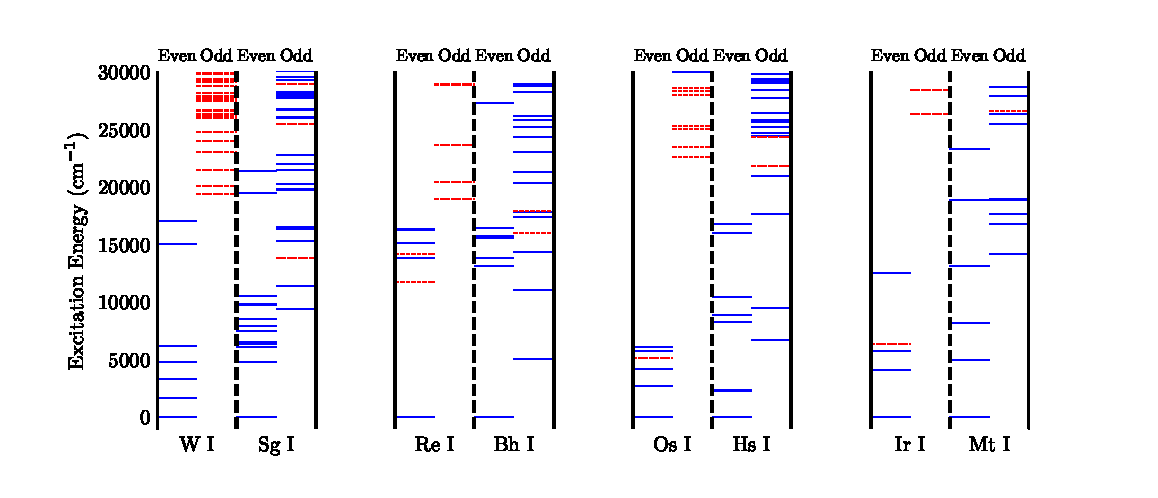
\includegraphics[scale=1]{./figures/Sg_Mt_Energy_Plot.eps} 
\caption[Low-energy excitation comparison between SHE and each respective lighter analog.]{Comparison of low-energy excitations of SHE and their respective lighter analogs. For each element, the states are split between odd and even parities. The solid (blue) lines represent states with $6s^2$ or $7s^2$ in the electronic configuration for the lighter elements and SHE respectively. The dashed (red) lines are all other states where an $s$ electron has been excited from the filled $6s$ or $7s$ shell. Experimental energies were used for W \textsc{i}, Bh \textsc{i}, Hs \textsc{i} and Ir \textsc{i}. \cite{NIST_ASD}\label{fig:EL}}
\end{figure}
\end{landscape}
Energy levels of SHE are calculated by solving the matrix eigenvalue problem (\ref{eq:CI}) separately for states of given value of the total angular momentum $J$ and parity. The specific details for each considered SHE are presented below. Most previous theoretical works on these SHE present the calculation of the first ionization potential, which we discuss in Section~\ref{sec:SHEIP}. Fig.~\ref{fig:EL} compares calculated spectra of low-lying states of SHE with experimental data on their lighter analogs. One can see a significant difference in the spectra of SHE and their lighter analogs, which is common for all considered atoms. Almost all low-lying odd states of lighter atoms correspond to the $6s-6p$ excitation from the ground state. In contrast to that, in SHE the $7s$ state is significantly lower on the energy scale than the $6d$ state due to relativistic effects. Therefore, dominant excitations occur from the $6d$ state, i.e. low-lying odd states correspond to the $6d-7p$ excitations from the ground state. Since the $6d-7p$ energy interval is smaller than the $6s-6p$ one, the density of odd states is higher for the SHE. 


\subsection{The Seaborgium Atom} \label{sec:Sg}


\afterpage{
\begin{longtable}{cl@{\hspace{0.5cm}}c@{\hspace{0.5cm}}r@{\hspace{0.5cm}}r} 
\caption[Low-energy spectrum of  Sg \textsc{i} calculated using the CIPT method]{Low-energy spectrum of even- and odd-parity states in Sg \textsc{i}.   We present the energy and Land\'e $g$-factor for each state $J^{\text{parity}}$. We present $LS$- notations only for comparison with lighter analogs.  For SHE states where an analogous state cannot be found in the lighter analog the term is labeled according to the sequential number of the state ($n$) for the given $J^{\text{parity}}$ group, $n_{J}^{\text{parity}}$.\label{tab:SHESpectrumSg}}
\endfirsthead
\multicolumn{5}{c}%
{\tablename\ \thetable\ -- \textit{Continued from previous page}} \\
\hline
&  \parbox{2cm}{Major \\ Configuration} & Term &   \parbox{1cm}{Energy \\ (cm$^{-1}$)}  &  \parbox{1.2cm}{Land\'{e} \\$g$-factor} \\
\hline
\endhead
\hline \multicolumn{5}{r}{\textit{Continued on next page}} \\
\endfoot
\endlastfoot
 		\toprule 
 \toprule 
&  \multicolumn{4}{c}{Sg \textsc{i}} \\
 \cmidrule{2-5} 
& \parbox{2cm}{Major \\ Configuration} & Term  &   \parbox{1cm}{Energy \\ (cm$^{-1}$)}  &  \parbox{1.2cm}{Land\'{e} \\$g$-factor}  \\ 
 		\midrule 
\multicolumn{5}{c}{Even parity states}\\
 (1) &  $6d^4 7s^2$ &  $^5$D$_0$    & 0 & 0.00   \\ 
 (2) &  $6d^4 7s^2$ &  $^5$D$_1$     & 4 834 & 1.50   \\ 
 (3) &  $6d^4 7s^2$ &  $^5$D$_2$    & 7 614 & 1.44   \\ 
 (4) &  $6d^4 7s^2$ &  $^5$D$_3$   & 9 607 & 1.39  \\  
 (5) &   $6d^4 7s^2$ &  $^5$D$_4$    & 10 335 & 1.27 \\ 
 (6) &  $6d^4 7s^2$ &  $^5$2P$_0$    & 13 592 & 0.00  \\  
\multicolumn{5}{c}{Odd parity states}\\
(7) &  $6d^3 7s^2 7p$  & 1$_2^{\rm_o}$    & 14 717 & 0.57   \\  
(8) &   $6d^3 7s^2 7p$  &  1$_1^{\rm_o}$    & 17 043 & 0.71  \\  
 (9) &  $6d^3 7s^2 7p$  & 2$_2^{\rm_o}$    & 20 444 & 1.13  \\  
(10) &   $6d^3 7s^2 7p$  & 1$_3^{\rm_o}$    & 20 628 & 0.97   \\  
(11) &  $6d^4 7s 7p$  &  $^7$F$_0^{\rm_o}$   & 20 979 & 0.00  \\  
(12) &  $6d^3 7s^2 7p$  & 2$_1^{\rm_o}$     & 22 041 & 2.02   \\  
 (13) &  $6d^3 7s^2 7p$  &  1$_4^{\rm_o}$   & 24 132 & 1.11  \\ 
(14) &  $6d^3 7s^2 7p$  & 3$_1^{\rm_o}$    & 24 382 & 1.19  \\  
(15) &  $6d^4 7s 7p$  &  $^1$S$_0^{\rm_o}$   & 25 362 & 0.00 \\  
 (16) &  $6d^3 7s^2 7p$  & 2$_3^{\rm_o}$  & 25 966 & 1.29   \\  
 (17) &  $6d^3 7s^2 7p$  &  1$_{5}^{\rm_o}$   & 26 271 & 1.17  \\ 
(18) &   $6d^3 7s^2 7p$  & 3$_2^{\rm_o}$     & 26 420 & 1.22  \\
(19) &  $6d^4 7s 7p$  &  $^7$F$_1^{\rm_o}$  & 27 030 & 1.40  \\ 
(20) & $6d^3 7s^2 7p$  & 4$_2^{\rm_o}$   & 27 416 & 1.74  \\ 
(21) & $6d^4 7s  7p $  &  $^7$F$_2^{\rm_o}$   & 29 976 & 1.41   \\ 
(22) & $6d^3 7s^2 7p$  &  3$_0^{\rm_o}$ & 30 055 & 0.00 \\
(23) & $6d^3 7s^2 7p$  &  2$_4^{\rm_o}$ & 30 372 & 1.25 \\
(24) & $6d^3 7s^2 7p$ & 3$_3^{\rm_o}$  & 30 753 & 1.09 \\
(25) & $6d^3 7s^2 7p$  & 5$_1^{\rm_o}$  & 30 868 & 0.92 \\
(26) & $6d^3 7s^2 7p$ & 4$_3^{\rm_o}$ & 31 647 & 1.34  \\
(27) & $6d^3 7s^2 7p$  & 6$_2^{\rm_o}$  & 32 040 & 1.13 \\
(28) & $6d^3 7s^2 7p$  &  3$_4^{\rm_o}$ & 32 073 & 1.00  \\
(29) & $6d^3 7s^2 7p$ &  4$_0^{\rm_o}$ & 32 381 & 0.00 \\
(30) & $6d^3 7s^2 7p$ &  6$_1^{\rm_o}$  & 32 520 & 1.21  \\
(31) & $6d^4 7s  7p $  &  $^5$D$_3^{\rm_o}$ & 32 885 & 1.47  \\
(32) & $6d^3 7s^2 7p$  &  4$_4^{\rm_o}$ & 33 339 & 1.23  \\
(33) & $6d^3 7s^2 7p$  & 7$_2^{\rm_o}$  & 33 602 & 1.08 \\
(34) & $6d^3 7s^2 7p$  & 8$_2^{\rm_o}$  & 34 147 & 1.45 \\
(35) & $6d^3 7s^2 7p$  &  2$_{5}^{\rm_o}$ & 34 380 & 1.12  \\  
(36) & $6d^3 7s^2 7p$  & 6$_3^{\rm_o}$  & 34 538 & 1.13  \\
(37) & $6d^3 7s^2 7p$  & 7$_1^{\rm_o}$  & 35 110 & 1.42 \\
(38) & $6d^3 7s^2 7p$  & 7$_3^{\rm_o}$  & 35 897 & 1.31  \\
(39) & $6d^3 7s^2 7p$  &  5$_4^{\rm_o}$ & 36 629 & 1.29  \\
(40) & $6d^3 7s^2 7p$  & 9$_2^{\rm_o}$  & 36 695 & 1.24 \\
(41) & $6d^3 7s^2 7p$ & 8$_3^{\rm_o}$  & 36 846 & 1.18 \\
(42) & $6d^3 7s^2 7p$  & 8$_1^{\rm_o}$  & 37 169 & 1.30 \\
(43) & $6d^3 7s^2 7p$  &  6$_4^{\rm_o}$& 37 218 & 1.25 \\
(44) & $6d^3 7s^2 7p$  &  3$_{5}^{\rm_o}$ & 37 542 & 1.26 \\
(45) & $6d^3 7s^2 7p$  &  5$_0^{\rm_o}$  & 38 322 & 0.00 \\ 
(46) & $6d^3 7s^2 7p$  & 9$_3^{\rm_o}$  & 38 547 & 1.12 \\ 
(47) & $6d^3 7s^2 7p$  & 10$_2^{\rm_o}$  & 38 915 & 1.22 \\ 
(48) & $6d^3 7s^2 7p$  &  7$_4^{\rm_o}$ & 39 138 & 1.30 \\
(49) & $6d^3 7s^2 7p$  &  4$_{5}^{\rm_o}$ & 39 337 & 1.23 \\
(50) & $6d^3 7s^2 7p$  & 10$_3^{\rm_o}$  & 39 725 & 1.23 \\
(51) & $6d^3 7s^2 7p$  & 9$_1^{\rm_o}$  & 40 073 & 1.62 \\ 
  \bottomrule
 \bottomrule
 \end{longtable} 
 }
Seaborgium was first experimentally detected in 1974 \cite{Ghoirso1974}. Since the initial discovery there has been continued interest and study into its physical and chemical properties including the discovery of isotopes with longer lifetimes. There exist some experimental results for Sg \textsc{i} in the field of chemistry \cite{Schadel2012}. However, there are no spectroscopic results available.   The ground state configuration of Sg \textsc{i} is expected to be [Rn]$5f^{14}6d^47s^2$, similar to the ground state of its lighter homologue (W \textsc{i}, ground configuration:  [Xe]$4f^{14}5d^46s^2$). \\
\linebreak
We calculated the first 6 even parity states and the ground state was found  to be the [Rn]$5f^{14}6d^47s^2 \ ^5$D$_0$ state. To calculate the even states we use three reference configurations, $6d^47s^2$, $6d^5 7s$ and $6d^6$ to make states in the effective CI matrix (first terms in the expansion (\ref{eq:psi}) and in the CI effective Hamiltonian (\ref{eq:HCI})). All other states, which are treated as corrections to the states from reference configurations (second terms in the expansion (\ref{eq:psi}) and in the CI Hamiltonian (\ref{eq:HCI})) are obtained by exciting one or two electrons from the reference configurations.
Similarly, for odd parity states we use the reference states from the $6d^47s7p$, $6d^37s^27p$ and $6d^57p$ configurations.  All calculated even and odd energy levels are presented in Table \ref{tab:SHESpectrumSgBh}. Similar calculations were performed for W~\textsc{i}  using analogous reference states and the same parameters. Comparing these results to the experimental spectrum~\cite{NIST_ASD} we found a maximum discrepancy of $|\Delta| \approx 600 $~cm$^{-1}$ and expect a similar accuracy for our Sg~\textsc{i} calculations. Note that this accuracy is slightly better than what was reported in Ref.~\cite{DBHF2017} due to inclusion of a larger number of states into the effective CI matrix.\\
\linebreak
Comparing the spectrum of Sg~\textsc{i} in Table~\ref{tab:SHESpectrumSg} to the spectrum of W~\textsc{I}~\cite{NIST_ASD}, we can see the manifestation of relativistic effects. As discussed above, relativistic effects cause the $7s$ orbital in Sg \textsc{i} to be strongly contracted and more tightly bound in comparison to the $6s$ orbital in W~\textsc{I}. The same effects also push out the $6d$ orbital of Sg \textsc{i} in comparison to the $5d$ orbital in W \textsc{i}. In the  W~\textsc{i} spectrum there are low-lying states corresponding to the $6s \rightarrow 5d$ excitation from the ground state (e.g., the $5d^56s \ ^7$S$_3$ state at 2 951.29 cm$^{-1}$). In contrast, in the Sg~\textsc{i} spectrum, all low-lying even states belong to the  $6d^4 7s^2$ configuration. The relativistic effects are more apparent in the low-lying odd parity states of Sg~\textsc{i}. In W~\textsc{i} all odd states correspond to the $6s \rightarrow 6p$ excitation from the ground state, while in Sg~\textsc{i} most of the low-lying odd states correspond to the $6d \rightarrow 7p$ excitation. Only a few of the Sg \textsc{i} predicted in the optical region correspond to the $7s \rightarrow 7p$ excitation.  \\
\linebreak
We calculate rates of electric dipole transitions from the ground state to excited states of the opposite parity using the approach described in Section~\ref{sec:Isoshift}. The results are presented in Table~\ref{tab:SHEE1transitionSg}. There are not many such transitions due to the zero value of the total angular momentum $J$ in the ground state. Because of that, the transitions are only allowed to the odd states with $J=1$. A few transitions are good candidates for the detection. The transition with the highest transition rate is $^5$D$_0 \rightarrow 9_1^{\rm_o}$ ($\omega = 40 \ 073 \text{ cm}^{-1}$).\\
\linebreak
We also present the isotopic shift parameters, $F$ and $a$ from equations (\ref{eq:isoa}) and (\ref{eq:isoF}), in Table~\ref{tab:SHEE1transitionSg} for each respective E1 transition. The two isotopes we use are $^{269}$Sg  and $^{290}$Sg ($R_{rms,\text{269}} = 5.8814$ fm and $R_{rms,\text{290}}  = 6.0145$ fm respectively),  where $^{290}$Sg is the theoretically  metastable ($N=184$) isotope of Sg. 

\subsection{The Bohrium Atom}  \label{sec:Bh}

 Bohrium was first discovered in 1981 \cite{Munzenberg1981}. No atomic spectra have been measured or calculated for any Bh isotopes or ions. When calculating the energy spectrum of Bh \textsc{i}, we use a similar approach as with Sg \textsc{i}.  For the low-lying even parity spectrum we use an effective CI matrix build from the states of the $6d^5 7s^2$, $6d^6 7s$ and $6d^7$ reference configurations. For the odd parity spectrum we use the states from the $6d^5 7s 7p$, $6d^4 7s^2 7p$ and $7d^6 7p$ reference configurations. The lowest six even parity states and low-lying odd parity states are presented in Table~\ref{tab:SHESpectrumBh}. For an estimate of accuracy we calculated the low-lying spectrum of Re~\textsc{i} (the lighter analogue of Bh) with similar parameters. Comparing the CIPT calculated spectrum to the experimental spectrum \cite{NIST_ASD}, the energy discrepancy (with respect to the ground state) was $\Delta \approx 900$~cm$^{-1}$ for the even parity states, while for the odd parity states $\Delta \approx 2000$~cm$^{-1}$.\\
\linebreak
\afterpage{
 \begin{longtable}{cl@{\hspace{0.5cm}}c@{\hspace{0.5cm}}r@{\hspace{0.5cm}}r} 

\caption[Low-energy spectrum of  Bh \textsc{i} calculated using the CIPT method]{Low-energy spectrum of even- and odd-parity states in Bh \textsc{i}.   We present the energy and Land\'e $g$-factor for each state $J^{\text{parity}}$. We present $LS$- notations only for comparison with lighter analogs.  For SHE states where an analogous state cannot be found in the lighter analog the term is labeled according to the sequential number of the state ($n$) for the given $J^{\text{parity}}$ group, $n_{J}^{\text{parity}}$.\label{tab:SHESpectrumBh}}
\endfirsthead
\multicolumn{5}{c}%
{\tablename\ \thetable\ -- \textit{Continued from previous page}} \\
\hline
&  \parbox{2cm}{Major \\ Configuration} & Term &   \parbox{1cm}{Energy \\ (cm$^{-1}$)}  &  \parbox{1.2cm}{Land\'{e} \\$g$-factor} \\
\hline
\endhead
\hline \multicolumn{5}{r}{\textit{Continued on next page}} \\
\endfoot
\endlastfoot
 		\toprule 
 \toprule 
&  \multicolumn{4}{c}{Bh \textsc{i}} \\
 \cmidrule{2-5}
&  \parbox{2cm}{Major \\ Configuration} & Term &   \parbox{1cm}{Energy \\ (cm$^{-1}$)}  &  \parbox{1.2cm}{Land\'{e} \\$g$-factor}  \\ 
 		\midrule 
\multicolumn{5}{c}{Even parity states}\\
 (1) &  $6d^5 7s^2$  &  $^6$S$_{5/2}$    & 0 & 1.78 \\ 
 (2) &   $6d^5 7s^2$  &  $^4$P$_{3/2}$    & 13 062 & 1.32 \\ 
 (3) &  $6d^5 7s^2$  &  $^4$G$_{7/2}$    &  13 828 & 1.15 \\ 
 (4) &   $6d^5 7s^2$  &  $^4$G$_{11/2}$    &  14 981 & 1.19 \\  
 (5) &   $6d^5 7s^2$  &  $^4$P$_{1/2}$   &  15 659 & 1.90 \\ 
 (6) &   $6d^5 7s^2$  &  $^4$G$_{9/2}$    & 16 447 & 1.17 \\  
\multicolumn{5}{c}{Odd parity states}\\
(7) &   $6d^4 7s^2 7p $  &  $^2$S$_{1/2}^{\rm_o}$    & 12 792 & 0.72 \\  
(8) &   $6d^4 7s^2 7p $   &  $^6$D$_{1/2}^{\rm_o}$   & 17 781 & 1.66 \\  
 (9) &   $6d^4 7s^2 7p $   &  $^6$D$_{3/2}^{\rm_o}$    & 19 483 & 1.09 \\  
(10) &   $6d^5 7s 7p$  &  $^8$P$_{5/2}^{\rm_o}$    & 22 228 & 2.08 \\  
(11) &   $6d^4 7s^2 7p $   &  $^6$P$_{3/2}^{\rm_o}$    & 22 533 & 1.74 \\  
(12) &   $6d^4 7s^2 7p $   &  $^6$D$_{5/2}^{\rm_o}$    & 22 930 & 1.26 \\  
 (13) &   $6d^5 7s 7p$  &  $^8$P$_{7/2}^{\rm_o}$    & 24 020 & 1.67 \\ 
(14)   &   $6d^4 7s^2 7p $   &  $^6$D$_{7/2}^{\rm_o}$    & 25 171 & 1.28 \\  
(15)  &   $6d^4 7s^2 7p $   &  $^6$D$_{9/2}^{\rm_o}$    & 26 587 & 1.21 \\  
 (16) &   $6d^4 7s^2 7p $  &  $^6$F$_{5/2}^{\rm_o}$    & 28 060 & 1.57 \\  
 (17) &  $6d^4 7s^2 7p $  & 3$_{1/2}^{\rm_o}$  & 29 823 & 0.44 \\ 
(18) &   $6d^4 7s^2 7p $ &  3$_{3/2}^{\rm_o}$  & 29 885 & 1.55 \\
(19) &  $6d^4 7s^2 7p $  & 3$_{7/2}^{\rm_o}$  & 31 078 & 1.24 \\ 
(20) &   $6d^4 7s^2 7p $ & 4$_{5/2}^{\rm_o}$  & 31 253 & 1.30 \\ 
(21) &   $6d^4 7s^2 7p $  & 4$_{7/2}^{\rm_o}$  & 32 814 & 1.37 \\ 
(22) &  $6d^4 7s^2 7p $  & 4$_{3/2}^{\rm_o}$  & 33 459 & 1.40 \\
(23) & $6d^4 7s^2 7p $  & 2$_{9/2}^{\rm_o}$  & 33 575 & 1.06 \\
(24) & $6d^4 7s^2 7p $  & 5$_{5/2}^{\rm_o}$     & 33 738 & 1.04 \\
(25) & $6d^4 7s^2 7p $  &  4$_{1/2}^{\rm_o}$  & 35 408 & 2.22 \\
(26) & $6d^4 7s^2 7p $  & 5$_{3/2}^{\rm_o}$   & 35 447 & 1.00 \\
(27) & $6d^4 7s^2 7p $  & 6$_{5/2}^{\rm_o}$  & 35 774 & 1.34 \\
(28) & $6d^4 7s^2 7p $  & 5$_{7/2}^{\rm_o}$   & 36 251 & 1.00 \\
(29) & $6d^4 7s^2 7p $  & 6$_{3/2}^{\rm_o}$    & 36 333 & 1.02 \\
(30) & $6d^4 7s^2 7p $  & 7$_{5/2}^{\rm_o}$    & 36 875 & 1.25 \\
(31) & $6d^4 7s^2 7p $  &  1$_{11/2}^{\rm_o}$    & 37 542 & 1.10 \\
(32) & $6d^4 7s^2 7p $  & 6$_{7/2}^{\rm_o}$  & 37 910 & 1.32 \\
(33)  & $6d^4 7s^2 7p $  & 7$_{3/2}^{\rm_o}$     & 37 954 & 1.05 \\
(34)  & $6d^5 7s 7p $  &  $^8$P$_{9/2}^{\rm_o}$    & 37 972 & 1.62 \\
(35) &  $6d^4 7s^2 7p $  & 4$_{9/2}^{\rm_o}$  & 38 336 & 1.23 \\  
(36) &  $6d^4 7s^2 7p $  & 8$_{5/2}^{\rm_o}$  & 39 454 & 1.19 \\
(37) &  $6d^4 7s^2 7p $  & 7$_{7/2}^{\rm_o}$  & 39 602 & 1.33 \\
(38) & $6d^4 7s^2 7p $  & 5$_{1/2}^{\rm_o}$  & 40 273 & 1.76 \\

  \bottomrule
 \bottomrule
 \end{longtable} 
 }
 The calculated Bh~\textsc{i} ground state is $6d^5 7s^2 \ ^6$S$_{5/2}$.  As with Sg~\textsc{i},  we see the relativistic effect of the tightly bound $7s$ electron which results in the primary excitation of the $6d$ electron. Comparing the spectrum of Bh~\textsc{i} with that of Re~\textsc{I} in Fig. \ref{fig:EL} we see that there are several low-lying states in Re~\textsc{I} corresponding to $6s \rightarrow 5d$ excitations (the lowest is at $11 754.52$~cm$^{-1}$), while there are no similar low-lying states in Bh~\textsc{i}.  The density of low-energy odd-parity states is much larger in Bh~\textsc{i} than in Re~\textsc{i}. The Bh \textsc{i} low odd-parity states are completely dominated by the $6d \rightarrow 7p$ excitations in calculated spectrum and and there are no  $7s \rightarrow 7p$ excitations. 
 The odd-parity state comparison between Bh~\textsc{i} and Re~\textsc{I} is similar to that of Sg~\textsc{i} and W~\textsc{i} in Section \ref{sec:Sg}. In the spectrum of Re~\textsc{i}~\cite{NIST_ASD} there do exist states corresponding to  $5d \rightarrow 6p$ transitions from the ground state; however, they occur much higher in the spectrum compared to Bh~\textsc{i} where the $6d \rightarrow 7p$ excitations dominate. It should be noted that the number of low-lying odd-parity states is larger in Bh~\textsc{i} than in Re \textsc{i}. The lowest odd state of Bh \textsc{i} occurs at $12 792$~cm$^{-1}$, whereas in Re~\textsc{i} the lowest odd state is at $18 950$~cm$^{-1}$.\\
 \linebreak
 Bh \textsc{i} has a large number of allowed low-energy optical E1 transitions from the ground state, which are presented  in Table \ref{tab:SHEE1transitionBh}. The isotope shift parameters, $a$ and $F$, are calculated using formulas (\ref{eq:isoa}) and (\ref{eq:isoF}) after calculating the atomic spectra for the theoretically meta-stable isotope of $^{270}$Bh using the CIPT method. We use the values of RMS nuclear radii  $ R_{rms,\text{270}} =  5.8879$ fm for $^{291}$Bh and $R_{rms,\text{291}} = 6.0207$ fm  for $^{291}$Bh.
 
\subsection{The Hassium atom} \label{sec:Hs}

Hassnium ($Z=108$) was first synthesized in 1984~\cite{Munzenberg1984}. We present the low-lying levels and the first ionization energy of Hs~\textsc{i} in Table~\ref{tab:SHESpectrumHs}. For the low-lying even spectrum effective CI reference states belong to the $6d^5 7s^2$, $6d^6 7s$ and $6d^7$ configurations. For the odd spectrum we use reference states of the $6d^5 7s 7p$, $6d^4 7s^2 7p$ and $7d^6 7p$ configurations.  Note that the half-filled $6d$ sub-shell makes computational methods particularly expensive. However, using the CIPT method the computation becomes tractable.  \\
\linebreak
Once again it is interesting to compare the spectra of Hs~\textsc{i} with the analogue Os~\textsc{i} in the period above. In the even states of Os~\textsc{i} there are states corresponding to the $6s \rightarrow 5d$ excitations from the ground state. In the Hs~\textsc{i} spectrum all low-lying even states belong to the  $6d^5 7s^2$ configuration. No states with the $7s \rightarrow 6d$ excitation were found. The odd states are similar to those of Sg and Bh, with the primary excitation $6d \rightarrow 7p$ in Hs~\textsc{i} while there are no  $5d \rightarrow 6s$ excitations in low Os~\textsc{i} spectrum. The odd states of Hs~\textsc{i} also lie much lower than those in Os~\textsc{i}.  The lowest odd state of Hs~\textsc{i} is 13 949 cm$^{-1}$, while the first odd state of Os~\textsc{i} occurs at 22 615.69 cm$^{-1}$ \cite{NIST_ASD}. 
\afterpage{
\begin{longtable}{cl@{\hspace{0.5cm}}c@{\hspace{0.5cm}}r@{\hspace{0.5cm}}r} 
\caption[Low-energy spectrum of  Hs \textsc{i} calculated using the CIPT method]{Low-energy spectrum of even- and odd-parity states in Hs \textsc{i}.   We present the energy and Land\'e $g$-factor for each state $J^{\text{parity}}$. We present $LS$- notations only for comparison with lighter analogs.  For SHE states where an analogous state cannot be found in the lighter analog the term is labeled according to the sequential number of the state ($n$) for the given $J^{\text{parity}}$ group, $n_{J}^{\text{parity}}$.\label{tab:SHESpectrumHs}}
\endfirsthead
\multicolumn{5}{c}%
{\tablename\ \thetable\ -- \textit{Continued from previous page}} \\
\hline
&  \parbox{2cm}{Major \\ Configuration} & Term &   \parbox{1cm}{Energy \\ (cm$^{-1}$)}  &  \parbox{1.2cm}{Land\'{e} \\$g$-factor} \\
\hline
\endhead
\hline \multicolumn{5}{r}{\textit{Continued on next page}} \\
\endfoot
\endlastfoot
 		\toprule 
 \toprule 
&  \multicolumn{4}{c}{Hs \textsc{i}} \\
 \cmidrule{2-5} 
& \parbox{2cm}{Major \\ Configuration} & Term  &   \parbox{1cm}{Energy \\ (cm$^{-1}$)}  &  \parbox{1.2cm}{Land\'{e} \\$g$-factor}  \\ 
 		\midrule 
  		 	\multicolumn{5}{c}{Even parity states}\\
 (1) &  $6d^6 7s^2$  &  $^5$D$_{4}$   & 0 & 1.37   \\ 
 (2) & $6d^6 7s^2$  &  $^5$D$_2$   & 2 102 & 1.38   \\  
 (3) &  $6d^6 7s^2$  &  $^5$D$_{0}$ & 7 400 & 0.00   \\ 
 (4) &  $6d^6 7s^2$  &  $^5$D$_{3}$ & 8 270 & 1.43   \\ 
 (5) &   $6d^6 7s^2$  &  $^5$D$_1$   & 9 285 & 1.41   \\ 
 (6) &    $6d^6 7s^2$  &  $^3$H$_{5}$ & 15 816 & 1.11\\ 
\multicolumn{5}{c}{Odd parity states}\\
  (7) &   $6d^5 7s^2 7p$  & 1$_2^{\rm_o}$    & 13 093 & 1.98  \\  
  (8) &  $6d^5 7s^2 7p$  & 1$_3^{\rm_o}$     & 15 600 & 1.58  \\ 
 (9) &  $6d^5 7s^2 7p$  & 2$_2^{\rm_o}$  & 23 708 & 1.30  \\ 
 (10) &  $6d^5 7s^2 7p$  & 2$_3^{\rm_o}$     & 26 492 & 1.16  \\ 
(11) &   $6d^6 7s 7p$  &  $^7$D$_{4}^{\rm_o}$   & 27 394 & 1.58  \\  
(12) &   $6d^5 7s^2 7p$  &  1$_1^{\rm_o}$   & 29 444 & 1.17  \\  
(13) &    $6d^5 7s^2 7p$  &  3$_2^{\rm_o}$    & 29 794 & 1.34  \\ 
(14) &   $6d^6 7s 7p$  &  $^7$D$_5^{\rm_o}$    &30 863 & 1.37   \\  
(15) &  $6d^5 7s^2 7p$  & 3$_3^{\rm_o}$     & 30 908 & 1.32  \\ 
(16) &   $6d^5 7s^2 7p$  & 4$_2^{\rm_o}$    & 31 165 & 1.33 \\ 
(17) &   $6d^5 7s^2 7p$  & 2$_4^{\rm_o}$      & 31 295 & 1.40   \\  
(18) &  $6d^5 7s^2 7p$  & 1$_0^{\rm_o}$  & 31 552 & 0.00  \\ 
(19) &  $6d^5 7s^2 7p$ & 3$_4^{\rm_o}$     & 32 522 & 1.26  \\ 
(20) &  $6d^5 7s^2 7p$ & 5$_2^{\rm_o}$   & 33 694 & 1.44  \\ 
(21) &  $6d^5 7s^2 7p$ & 4$_3^{\rm_o}$     & 33 920 & 1.03 \\ 
(22) &  $6d^5 7s^2 7p$ & 2$_1^{\rm_o}$      & 34 076 & 1.52 \\ 
(23) &  $6d^5 7s^2 7p$  & 2$_5^{\rm_o}$     & 34 739 & 1.20 \\ 
(24) &  $6d^5 7s^2 7p$ & 5$_3^{\rm_o}$   & 34 812 & 1.41 \\
(25) &  $6d^5 7s^2 7p$ & 4$_4^{\rm_o}$   & 35 689 & 1.23 \\ 
(26) &  $6d^6 7s 7p$  &  $^7$D$_{3}^{\rm_o}$  & 35 705 & 1.56 \\ 
(27) &  $6d^5 7s^2 7p$  & 3$_1^{\rm_o}$   & 35 990 & 1.81 \\ 
(28) &  $6d^6 7s 7p$  &  $^7$D$_2^{\rm_o}$  & 37 036 & 1.40 \\ 
(29) &  $6d^6 7s 7p$  & $^7$P$_{3}^{\rm_o}$ & 37 237 & 1.33 \\ 
(30) &  $6d^5 7s^2 7p$ & 5$_4^{\rm_o}$   & 37 443 & 1.18 \\ 
(31) &  $6d^5 7s^2 7p$ & 7$_2^{\rm_o}$   & 38 519 & 1.34 \\
(32) &  $6d^6 7s 7p$  &  $^7$P$_{4}^{\rm_o}$ & 39 025 & 1.29 \\ 
(33) &  $6d^5 7s^2 7p$  & 3$_5^{\rm_o}$   & 39 268 & 1.27 \\
(34) &  $6d^6 7s 7p$  &  $^7$D$_1^{\rm_o}$  & 39 512 & 2.11 \\ 
(35) &  $6d^5 7s^2 7p$  & 8$_3^{\rm_o}$  & 39 652 & 1.38 \\ 
(36) &  $6d^5 7s^2 7p $  & 9$_3^{\rm_o}$    &  40 783  &  1.19 \\
  \bottomrule
 \bottomrule
 \end{longtable} 
 }
The allowed strong optical E1 transitions from the low-lying odd states to the ground state ($^5$D$_{4}$) are presented in Table~\ref{tab:SHEE1transitionHs}. As with Bh \textsc{i} there is a large number of strong optical transitions. The transition with the largest rate is 3$_5^{\rm o}$ $\rightarrow$ $^5$D$_{4}$ ($\omega =$~39~268~cm$^{-1}$). Other possibly detectable transitions include 5$_3^{\circ}$ $\rightarrow$ $^5$D$_{4}$ ($\omega =$~34~812~cm$^{-1}$) and 2$_5^{\circ}$ $\rightarrow$ $^5$D$_{4}$ ($\omega= $~34~739~cm$^{-1}$).

We also present the isotopic shift parameters for the Hs E1 optical transitions in Table~\ref{tab:SHEE1transitionHs}. These were calculated from the theoretical spectra (calculated with the CIPT method) with isotopes $^{270}$Hs and $^{292}$Hs with RMS nuclear radii $R_{rms,\text{270}} = 5.8879$ fm for $^{292}$Hs and $R_{rms,\text{292}} = 6.0207$ fm for $^{270}$Hs.

\subsection{The Meitnerium Atom} \label{sec:Mt}


 
 \afterpage{
\begin{longtable}{cl@{\hspace{0.5cm}}c@{\hspace{0.5cm}}r@{\hspace{0.5cm}}r} 
\caption[Low-energy spectrum of  Mt \textsc{i} calculated using the CIPT method]{Low-energy spectrum of even- and odd-parity states in Mt \textsc{i}.   We present the energy and Land\'e $g$-factor for each state $J^{\text{parity}}$. We present $LS$- notations only for comparison with lighter analogs.  For SHE states where an analogous state cannot be found in the lighter analog the term is labeled according to the sequential number of the state ($n$) for the given $J^{\text{parity}}$ group, $n_{J}^{\text{parity}}$.\label{tab:SHESpectrumMt}}
\endfirsthead
\multicolumn{5}{c}%
{\tablename\ \thetable\ -- \textit{Continued from previous page}} \\
\hline
&  \parbox{2cm}{Major \\ Configuration} & Term &   \parbox{1cm}{Energy \\ (cm$^{-1}$)}  &  \parbox{1.2cm}{Land\'{e} \\$g$-factor} \\
\hline
\endhead
\hline \multicolumn{5}{r}{\textit{Continued on next page}} \\
\endfoot
\endlastfoot
 		\toprule 
 \toprule 
&  \multicolumn{4}{c}{Mt \textsc{i}} \\
 \cmidrule{2-5} 
& \parbox{2cm}{Major \\ Configuration} & Term  &   \parbox{1cm}{Energy \\ (cm$^{-1}$)}  &  \parbox{1.2cm}{Land\'{e} \\$g$-factor}  \\ 
 		\midrule 
  		 	\multicolumn{5}{c}{Even parity states}\\
 (1) & $6d^7 7s^2$  &  $^4$F$_{9/2}$ & 0 & 1.265 \\ 
 (2) &  $6d^7 7s^2$  &  $^4$F$_{3/2}$  & 5 047 & 1.214 \\  
 (3) &   $6d^7 7s^2$  &  $^4$F$_{5/2}$ & 7 996 & 1.222 \\ 
 (4) &   $6d^7 7s^2$  &  $^4$F$_{7/2}$ & 12 628 & 1.213 \\ 
 (5) &   $6d^7 7s^2$  &  $^2$G$_{3/2}$ & 17 368 & 0.931 \\ 
 (6) & $6d^7 7s^2$  &  $^2$G$_{5/2}$   & 18 467 & 1.409\\ 
\multicolumn{5}{c}{Odd parity states}\\
  (7) &   $6d^6 7s^2 7p $  & 1$_{7/2}^{\rm_o}$   & 21 879 & 1.44 \\  
  (8) &   $6d^6 7s^2 7p $  &  1$_{9/2}^{\rm_o}$ & 24 388 & 1.33 \\ 
 (9) &   $6d^6 7s^2 7p $  & 1$_{3/2}^{\rm_o}$  & 24 524 & 1.51 \\ 
 (10) &   $6d^6 7s^2 7p $ & 1$_{5/2}^{\rm_o}$   & 25 990 & 1.25 \\ 
(11)  &   $6d^6 7s^2 7p $  & 2$_{5/2}^{\rm_o}$   & 31 975 & 1.54 \\  
(12) &  $6d^6 7s^2 7p $  &1$_{1/2}^{\rm_o}$    & 32 851 & 0.81 \\  
(13) &  $6d^7 7s  7p$  &  $^{6}$D$_{9/2}^{\rm_o}$ & 33 505 & 1.40 \\ 
(14) &  $6d^6 7s^2 7p $  & 2$_{1/2}^{\rm_o}$   & 34 665 & 1.51\\  
(15) &   $6d^6 7s^2 7p$  & 2$_{7/2}^{\rm_o}$    & 35 117 & 1.29 \\ 
(16) &   $6d^6 7s^2 7p$  & 2$_{3/2}^{\rm_o}$     & 36 159 & 1.13 \\ 
(17) &   $6d^7 7s 7p$  &  $^6$F$_{11/2}^{\rm_o}$   & 38 027 & 1.31 \\  
(18) &   $6d^6 7s^2 7p$& 3$_{7/2}^{\rm_o}$   & 38 450 & 1.17 \\ 
(19) & $6d^6 7s^2 7p$  & 3$_{9/2}^{\rm_o}$    & 39 296 & 1.13 \\ 
(20) & $6d^6 7s^2 7p$  & 2$_{11/2}^{\rm_o}$     & 41 310 & 1.33 \\ 
 \bottomrule
 \bottomrule

 \end{longtable} 
 }
Meitnerium ($Z=109$) was first synthesized in 1982 \cite{Munzenberg1982}. The ground state of Mt~\textsc{i} is expected to follow that of the element in the above period  (Ir) with [Rn]$5f^{14}6d^{7}7s^2 \ ^4$F$_{9/2}$ which we confirm in the calculated spectrum presented in Table \ref{tab:SHESpectrumMt}.\\
\linebreak
We use the same method as for previous elements to calculate the low-lying spectrum of Mt~\textsc{i}. We present the lowest six even states using the  $6d^7 7s^2$, $6d^8, 7s$ and $6d^9$ reference configurations. We also present the first 12 odd parity states for which the $6d^7 7s 7p$, $6d^6 7s^2 7p$ and $6d^8 7p$ configurations were used. The results are in Table~\ref{tab:SHESpectrumMt}. Comparison with lighter analog Ir~\textsc{i} shows similar trend as for other SHE Sg, Bh and Hs. \\
\linebreak
 We also present the allowed E1 transitions for Mt and the respective isotope shift parameters in Table~ \ref{tab:SHEE1transitionMt}. The high energy of the odd states in Mt~\textsc{i} result in a small number of allowed E1 transitions within optical region from the ground state compared to Bh and Hs.  Promising transitions for future measurement include $^6$F$_{11/2}^{\circ} \rightarrow ^4$F$_{9/2}$ ($\omega =$~38~027~cm$^{-1}$) and $^{6}$D$_{9/2}^{\circ} \rightarrow ^4$F$_{9/2}$ ($\omega =$ 33~505~cm$^{-1}$). All other rates are two or more orders of magnitude smaller. For the synthesized and metastable isotopes we use the RMS nuclear radii values, $R_{rms,\text{276}} = 5.9265$ fm  and $R_{rms,\text{293}} = 6.0330$ fm.
 
 \afterpage{
\begin{longtable}{l@{\hspace{0.01cm}}c@{\hspace{0.5cm}}r@{\hspace{0.5cm}}r@{\hspace{0.5cm}}r@{\hspace{0.5cm}}r@{\hspace{0.5cm}}r} 
 \caption[Electric dipole transitions and isotopic shift parameters for Sg \textsc{i} using the CIPT method]{Strong electric dipole transitions and isotopic shift parameters for Sg \textsc{i}. Only direct optical transitions to the ground state satisfying the E1 transition selection rules are shown. Here $D_{\text{E1}}$ is the transition amplitude in a.u., $A_{\text{E1}}$ is the transition rate, $a$, $F$, and $\tilde{F}$ are calculated isotopic shift parameters for the charge radius. The numbers in parentheses correspond to the numbered states in Table \ref{tab:SHESpectrumSg}. \label{tab:SHEE1transitionSg}}
\endfirsthead
\multicolumn{5}{c}%
{\tablename\ \thetable\ -- \textit{Continued from previous page}} \\
\hline
& State &   \parbox{1cm}{$D_{\text{E1}}$ \\ (a.u)} & \parbox{1cm}{$A_{\text{E1}}$ \\ { \small $(\times 10^{6} \ \text{s}^{-1})$ }} & \parbox{1cm}{$a  $ \\ (cm$^{-1}$)} & \parbox{1cm}{$F $ \\ ($\frac{\text{cm}^{-1}}{\text{fm}^{2}}$)} &   \multicolumn{1}{c}{\parbox{1cm}{$\tilde{F} $ \\ (cm$^{-1}$) }} \\
\hline
\endhead
\hline \multicolumn{5}{r}{\textit{Continued on next page}} \\
\endfoot
\endlastfoot
\toprule
\toprule
& State &   \parbox{1cm}{$D_{\text{E1}}$ \\ (a.u)} & \parbox{1cm}{$A_{\text{E1}}$ \\ { \small $(\times 10^{6} \ \text{s}^{-1})$ }} & \parbox{1cm}{$a  $ \\ (cm$^{-1}$)} & \parbox{1cm}{$F $ \\ ($\frac{\text{cm}^{-1}}{\text{fm}^{2}}$)} &   \multicolumn{1}{c}{\parbox{1cm}{$\tilde{F} $ \\ (cm$^{-1}$) }} \\
\midrule
 		\multicolumn{7}{c}{Sg \textsc{i} (Ground state: $^5$D$_0$)}  \\
 		\\
(8) &  1$_1^{\rm_o}$        & 0.639 & 1.36 & 9.41& 2.04 & 11.9   \\ 
(12) & 2$_{1}^{\rm_o}$          & -0.160 & 0.192 & -2.95 & -0.639 & -3.73 \\ 
(14) & 3$_{1}^{\rm_o}$         & 1.17  & 13.4 & 4.90 & 1.06 & 6.18  \\ 
(19) & $^3$P$_1^{\rm_o}$      & -0.163 & 0.353 & -19.7 & -4.25 & -24.8  \\ 
(25) & 5$_{1}^{\rm_o}$   & 0.592 & 6.97 & 6.58 & 1.42 & 8.30  \\ 
(30) &  6$_{1}^{\rm_o}$     & -0.412 & 3.95 & 7.01 & 1.52 & 8.85  \\ 
(37) &  7$_{1}^{\rm_o}$ & -0.302 & 2.67&  1.66 & 0.36 & 2.10  \\
 (42) & 8$_{1}^{\rm_o}$   & 0.148& 0.761 & 3.55 & 0.768 & 4.48  \\
(51) & 9$_{1}^{\rm_o}$   & 0.524 & 11.9 & -4.77& -1.03& -6.01 \\
\bottomrule
\bottomrule
\end{longtable}
}

\afterpage{
\begin{longtable}{l@{\hspace{0.01cm}}c@{\hspace{0.5cm}}r@{\hspace{0.5cm}}r@{\hspace{0.5cm}}r@{\hspace{0.5cm}}r@{\hspace{0.5cm}}r}   % @{} adds extra padding to the columns 
 \caption[Electric dipole transitions and isotopic shift parameters for Bh \textsc{i} using the CIPT method]{Strong electric dipole transitions and isotopic shift parameters for Bh \textsc{i}. Only direct optical transitions to the ground state satisfying the E1 transition selection rules are shown. Here $D_{\text{E1}}$ is the transition amplitude in a.u., $A_{\text{E1}}$ is the transition rate, $a$, $F$, and $\tilde{F}$ are calculated isotopic shift parameters for the charge radius. The numbers in parentheses correspond to the numbered states in Table \ref{tab:SHESpectrumBh}. \label{tab:SHEE1transitionBh}}
\endfirsthead
\multicolumn{5}{c}%
{\tablename\ \thetable\ -- \textit{Continued from previous page}} \\
\hline
& State &   \parbox{1cm}{$D_{\text{E1}}$ \\ (a.u)} & \parbox{1cm}{$A_{\text{E1}}$ \\ { \small $(\times 10^{6} \ \text{s}^{-1})$ }} & \parbox{1cm}{$a  $ \\ (cm$^{-1}$)} & \parbox{1cm}{$F $ \\ ($\frac{\text{cm}^{-1}}{\text{fm}^{2}}$)} &   \multicolumn{1}{c}{\parbox{1cm}{$\tilde{F} $ \\ (cm$^{-1}$) }} \\
\hline
\endhead
\hline \multicolumn{5}{r}{\textit{Continued on next page}} \\
\endfoot
\endlastfoot
\toprule
\toprule
& State &   \parbox{1cm}{$D_{\text{E1}}$ \\ (a.u)} & \parbox{1cm}{$A_{\text{E1}}$ \\ { \small $(\times 10^{6} \ \text{s}^{-1})$ }} & \parbox{1cm}{$a  $ \\ (cm$^{-1}$)} & \parbox{1cm}{$F $ \\ ($\frac{\text{cm}^{-1}}{\text{fm}^{2}}$)} &   \multicolumn{1}{c}{\parbox{1cm}{$\tilde{F} $ \\ (cm$^{-1}$) }} \\
\midrule
 \multicolumn{7}{c}{Bh \textsc{i} (Ground State: $^6$S$_{5/2}$)} \\
 		\\
(9)  & $^6$D$_{3/2}^{\rm_o}$     & -0.172 & 0.107 & 18.1 & 3.74 & 22.8  \\ 
(10) & $^8$P$_{5/2}^{\rm_o}$     & -0.474 &  0.812 & 83.4 & 17.2 & 105 \\ 
(11) &  $^6$P$_{3/2}^{\rm_o}$     & -0.494 & 1.38 & -101 & -20.7 & -127 \\ 
(12) &  $^6$D$_{5/2}^{\rm_o}$     & -0.0391 & 0.00611 & -120 & -24.6 & -151 \\ 
(13)  & $^8$P$_{7/2}^{\rm_o}$     & 0.500 & 0.858 & 84.5 & 17.4 & 107 \\ 
(14)  & $^6$D$_{7/2}^{\rm_o}$     & 0.345 & 0.471 & -63.3 & -13.0 & -79.7 \\ 
(16) & $^6$F$_{5/2}^{\rm_o}$     & 1.51 & 16.6 & -160 & -33.0 & -202 \\
(18)  & 3$_{3/2}^{\rm_o}$  & 1.50 & 30.0 & -64.9 & -13.4 & -81.7 \\
(19) & 3$_{7/2}^{\rm_o}$   & 1.75 & 23.3 & 44.0 & 9.06& 55.4 \\
(20) & 4$_{5/2}^{\rm_o}$   &  -0.433 & 1.90 & -101 & -20.7 & -127  \\
(21) & 4$_{7/2}^{\rm_o}$   &  1.88 & 31.2 & -380 & -78.4 & -479 \\
(22) & 4$_{3/2}^{\rm_o}$  &   -0.998 & 18.6 & -41.3 & -8.51& -52 \\
(24) & 5$_{5/2}^{\rm_o}$  &   -0.101 & 0.131 & -105 & -21.6 & -132 \\
(26) & 5$_{3/2}^{\rm_o}$   &   0.438 & 4.27 & -135 & -27.9 & -170 \\
(27) & 6$_{5/2}^{\rm_o}$  &   -1.06 & 17.1 & -364 & -74.9 & -458 \\
(28) & 5$_{7/2}^{\rm_o}$  &  0.0665 & 0.0361 & -34.7 & -7.15 & -43.7 \\
(29) & 6$_{3/2}^{\rm_o}$    &  0.160 & 0.615 & -70.6 & -14.5 & -88.9 \\
(30) & 7$_{5/2}^{\rm_o}$    &  -0.539 & 4.86 & -335 & -69.0 & -422\\
(33) & 6$_{7/2}^{\rm_o}$   &   -0.674 & 6.18 & -129 & -26.6 & -163 \\
(34) & 7$_{3/2}^{\rm_o}$   &  0.387 & 4.09 & -513 & -106 & -647 \\
(37) & 8$_{5/2}^{\rm_o}$   &  0.232 & 1.10 & -561 & -116 & -707\\
(38) & 7$_{7/2}^{\rm_o}$  &  0.516 & 4.13 & -364 & -75.1 & -459 \\
\bottomrule
\bottomrule
\end{longtable}
}

\afterpage{
\begin{longtable}{l@{\hspace{0.01cm}}c@{\hspace{0.5cm}}r@{\hspace{0.5cm}}r@{\hspace{0.5cm}}r@{\hspace{0.5cm}}r@{\hspace{0.5cm}}r}   % @{} adds extra padding to the columns 
 \caption[Electric dipole transitions and isotopic shift parameters for Hs \textsc{i} using the CIPT method]{Strong electric dipole transitions and isotopic shift parameters for Hs~\textsc{i}. Only direct optical transitions to the ground state satisfying the E1 transition selection rules are shown. Here $D_{\text{E1}}$ is the transition amplitude in a.u., $A_{\text{E1}}$ is the transition rate, $a$, $F$, and $\tilde{F}$ are calculated isotopic shift parameters for the charge radius. The numbers in parentheses correspond to the numbered states in Table \ref{tab:SHESpectrumHs}. \label{tab:SHEE1transitionHs}}
\endfirsthead
\multicolumn{5}{c}%
{\tablename\ \thetable\ -- \textit{Continued from previous page}} \\
\hline
& State &   \parbox{1cm}{$D_{\text{E1}}$ \\ (a.u)} & \parbox{1cm}{$A_{\text{E1}}$ \\ { \small $(\times 10^{6} \ \text{s}^{-1})$ }} & \parbox{1cm}{$a  $ \\ (cm$^{-1}$)} & \parbox{1cm}{$F $ \\ ($\frac{\text{cm}^{-1}}{\text{fm}^{2}}$)} &   \multicolumn{1}{c}{\parbox{1cm}{$\tilde{F} $ \\ (cm$^{-1}$) }} \\
\hline
\endhead
\hline \multicolumn{5}{r}{\textit{Continued on next page}} \\
\endfoot
\endlastfoot
\toprule
\toprule
& State &   \parbox{1cm}{$D_{\text{E1}}$ \\ (a.u)} & \parbox{1cm}{$A_{\text{E1}}$ \\ { \small $(\times 10^{6} \ \text{s}^{-1})$ }} & \parbox{1cm}{$a  $ \\ (cm$^{-1}$)} & \parbox{1cm}{$F $ \\ ($\frac{\text{cm}^{-1}}{\text{fm}^{2}}$)} &   \multicolumn{1}{c}{\parbox{1cm}{$\tilde{F} $ \\ (cm$^{-1}$) }} \\
\midrule
 		\multicolumn{7}{c}{Hs \textsc{i} (Ground State: $^5$D$_{4}$)} \\
 		\\
(8)  & 1$_{3}^{\rm_o}$     & 0.501 &  0.276 & 22.7 & 4.45 & 28.9 \\
(10) & 2$_{3}^{\rm_o}$      & 0.224 & 0.269 & 22.9 & 4.49 & 28.8  \\
(11) & $^7$D$_{4}^{\rm_o}$    & -1.11 & 5.66 & -29.1 & -5.70 & -36.6   \\
(14) & $^7$D$_5^{\rm_o}$     & 0.999 &  5.41& -26.2 & -5.15  \\
(15) & 3$_{3}^{\rm_o}$     & 0.208 & 0.370 & 16.2 & 3.18 & 20.4   \\
(17) & 2$_{4}^{\rm_o}$      & 0.0934 & 0.0603 & 5.54 & 1.09 & 6.98   \\ 
(19) & 3$_{4}^{\rm_o}$      & 0.120 & 0.112 & 18.5 & 3.62 & 23.2   \\
(21) & 4$_{3}^{\rm_o}$      & -0.150 & 0.253 & 20.7 & 4.05 & 26.0  \\
(23) & 2$_{5}^{\rm_o}$      & -1.13 & 9.88 & 12.3 & 2.42 & 15.5   \\
 (24) & 5$_{3}^{\rm_o}$    & 1.70 & 35.5 & 12.3 & 2.41 & 15.5  \\
(25) & 4$_{4}^{\rm_o}$      & 0.798 & 6.52 & 7.84 & 1.54 & 9.87  \\ 
(26)  &  $^7$D$_{3}^{\rm_o}$   & -0.493 & 3.20 & -33.3 & -6.53 & -41.9  \\ 
(29) & $^7$P$_{3}^{\rm_o}$  & -0.511 & 3.91 & -15.8 & -3.11 & -19.9  \\ 
(30) &5$_{4}^{\rm_o}$     & -0.297 & 1.04 & 1.95 & 0.382 & 2.45  \\ 
(32) & $^7$P$_{4}^{\rm_o}$  & 0.425 &  2.41 & -9.56 & -1.87 & -12.0 \\ 
(33) &3$_{5}^{\rm_o}$     & 2.64 & 77.5 & 5.16 & 1.01 & 6.49   \\ 
(35) & 7$_{3}^{\rm_o}$    & 2.10 & 80.0 & -2.30 & -0.451 & -2.89  \\ 
\bottomrule
\bottomrule
\end{longtable}
}


 \afterpage{
\begin{longtable}{l@{\hspace{0.01cm}}c@{\hspace{0.5cm}}r@{\hspace{0.5cm}}r@{\hspace{0.5cm}}r@{\hspace{0.5cm}}r@{\hspace{0.5cm}}r}   % @{} adds extra padding to the columns 
 \caption[Electric dipole transitions and isotopic shift parameters for Mt \textsc{i} using the CIPT method]{Strong electric dipole transitions and isotopic shift parameters for Mt~\textsc{i}. Only direct optical transitions to the ground state satisfying the E1 transition selection rules are shown. Here $D_{\text{E1}}$ is the transition amplitude in a.u., $A_{\text{E1}}$ is the transition rate, $a$, $F$, and $\tilde{F}$ are calculated isotopic shift parameters for the charge radius. The numbers in parentheses correspond to the numbered states in Table \ref{tab:SHESpectrumMt}. \label{tab:SHEE1transitionMt}}
\endfirsthead
\multicolumn{5}{c}%
{\tablename\ \thetable\ -- \textit{Continued from previous page}} \\
\hline
& State &   \parbox{1cm}{$D_{\text{E1}}$ \\ (a.u)} & \parbox{1cm}{$A_{\text{E1}}$ \\ { \small $(\times 10^{6} \ \text{s}^{-1})$ }} & \parbox{1cm}{$a  $ \\ (cm$^{-1}$)} & \parbox{1cm}{$F $ \\ ($\frac{\text{cm}^{-1}}{\text{fm}^{2}}$)} &   \multicolumn{1}{c}{\parbox{1cm}{$\tilde{F} $ \\ (cm$^{-1}$) }} \\
\hline
\endhead
\hline \multicolumn{5}{r}{\textit{Continued on next page}} \\
\endfoot
\endlastfoot
\toprule
\toprule
& State &   \parbox{1cm}{$D_{\text{E1}}$ \\ (a.u)} & \parbox{1cm}{$A_{\text{E1}}$ \\ { \small $(\times 10^{6} \ \text{s}^{-1})$ }} & \parbox{1cm}{$a  $ \\ (cm$^{-1}$)} & \parbox{1cm}{$F $ \\ ($\frac{\text{cm}^{-1}}{\text{fm}^{2}}$)} &   \multicolumn{1}{c}{\parbox{1cm}{$\tilde{F} $ \\ (cm$^{-1}$) }} \\
\midrule
\multicolumn{7}{c}{Mt \textsc{i} (Ground State: $^4$F$_{9/2}$)}\\
 		\\
 (7)	& 1$_{7/2}^{\rm_o}$	  & 0.0537 & 0.00765 & 27.5& 5.10 & 34.5 \\
   (8)	& 1$_{9/2}^{\rm_o}$	 & 0.432 & 0.550 & 27.6 & 5.13 & 34.7 \\
 (13)	&	$^{6}$D$_{9/2}^{\rm_o}$  & 1.27 & 12.3 & -51.7 & -9.60 & -64.9  \\
  (15) & 2$_{7/2}^{\rm_o}$	   & -0.294 & 0.946 & 33.3 & 6.18 & 41.8 \\
 (17)	&	$^6$F$_{11/2}^{\rm_o}$    & -1.89 & 33.3 & -47.9& -8.89& -60.1 \\
  (19) 	& 3$_{9/2}^{\rm_o}$	    & 0.0954 & 0.112 & 19.0 & 3.53 & 23.9  \\ 
 (20) 	& 2$_{11/2}^{\rm_o}$	    & 0.170 & 0.344 & 25.7 & 4.78 & 32.3  \\
\bottomrule
\bottomrule
\end{longtable}
}


\section{Ionization potentials and comparison with other data.} \label{sec:SHEIP}

As well as calculating the spectrum of neutral Sg, Bh, Hs and Mt we also calculated their first ionization potentials (IPs). To calculate the IP for each atom we use the same single-electron basis set for a neutral atom and an ion. The ionization potential is found as a difference between ground state energies of the atom and its ion. The effective CI matrix was built from all states of the $6d^n 7s$, $6d^{n-1}7s^2$ and $6d^{n+1}$ reference configurations ($n=4-7$ for Sg through to Mt). States that were treated perturbatively were obtained by exciting one or two electrons from the reference configurations and generating all single-determinant states from these configurations. We start from calculating the IPs of lighter analogs of the SHE to compare them with experiment. The results are in Table~\ref{tab:IP}. We also include in the table the results of the multi-configuration Dirac-Fock (MCDF) calculation~\cite{Johnson1999, Johnson2002}. We do this because similar MCDF calculations have been used for the SHE (see Tables~\ref{tab:EE} and \ref{tab:SHEIP}). The CIPT values of the IPs agree with experiment within few percent (error $<$1\% for Ta, W, and Re, and $\sim$ 3\% for Os and Ir). We expect similar accuracy for the first IPs of SHE analogs presented in Table \ref{tab:SHEIP}.  For comparison, the difference between MCDF values of IPs of W, Re and Os and experimental IPs is larger than 10\% (Table~\ref{tab:IP}).
 \afterpage{
\begin{longtable}{llcccc}
\caption[Theoretical and experimental ionization potentials of open $5d$-shell elements.]{Theoretical and experimental ionization potentials of open $5d$-shell elements.  The CIPT energies are the results of the present work. \label{tab:IP}}
\endfirsthead
\multicolumn{5}{c}%
{\tablename\ \thetable\ -- \textit{Continued from previous page}} \\
\hline
           &                  & \multicolumn{3}{c}{IP (eV)} \\
Atom &  \parbox{1cm}{Ionic \\ State} & $J$ &  Expt.~\cite{NIST_ASD}   & CIPT  & MCDF \\
\hline
\endhead
\hline \multicolumn{5}{r}{\textit{Continued on next page}} \\
\endfoot
\endlastfoot
           &                  & \multicolumn{3}{c}{IP (eV)} \\
Atom &  \parbox{1cm}{Ionic \\ State} & $J$ &  Expt.~\cite{NIST_ASD}   & CIPT  & MCDF \\
\toprule
\toprule
Ta    & $5d^3 6s$  & 1   & 7.549    & 7.57  & \\
W     & $5d^4 6s$ & 1/2 & 7.864   & 7.90  &  6.97~\cite{MCDF-Sg}  \\
Re    & $5d^5 6s$ & 3   &  7.833  &  7.85  &  6.84~\cite{MCDF-BhHs} \\
Os    & $5d^6 6s$ & 9/2 & 8.438  &  8.69  &  7.45~\cite{MCDF-BhHs} \\
Ir      & $5d^7 6s$ & 5    & 8.967 &  9.27  & \\
\bottomrule
\bottomrule
\end{longtable}
}

Table~\ref{tab:EE} shows some resonance (corresponding to strong electric dipole transitions from the ground state) excitation energies for SHE and their lighter analogs calculated in the present work and by the MCDF method~\cite{MCDF-Sg,MCDF-BhHs}. The energies for lighter elements are compared to experiment. Our values are taken from Tables~\ref{tab:SHESpectrumSg}, \ref{tab:SHESpectrumBh}, \ref{tab:SHESpectrumHs} and \ref{tab:SHESpectrumMt}; for the MCDF energies we present all results which can be found in~\cite{MCDF-Sg,MCDF-BhHs}. There is  a significant difference in the excitation energies of SHE, while for lighter atoms the difference is not so large. There is a $\sim$ 10\% difference from experiment in both calculations. There are too little data on the MCDF calculations to come to any conclusion about the reasons for the differences. %We believe that our results for excitation energies of SHE are more accurate because there are more carefully verified 
\afterpage{
\begin{longtable}{lllccc}
\caption[Some excitation energies in open $6d$-shell SHE and each lighter analog]{Some excitation energies (cm$^{-1}$) in open $6d$-shell SHE and their lighter analogs. The CIPT energies are the results of the present work.   \label{tab:EE}}
\endfirsthead
\multicolumn{5}{c}%
{\tablename\ \thetable\ -- \textit{Continued from previous page}} \\
\hline
Atom &  \multicolumn{2}{c}{State} &  Expt.~\cite{NIST_ASD}   & CIPT  & MCDF~\cite{MCDF-Sg,MCDF-BhHs} \\
\hline
\endhead
\hline \multicolumn{5}{r}{\textit{Continued on next page}} \\
\endfoot
\endlastfoot
\toprule
\toprule
Atom &  \multicolumn{2}{c}{State} &  Expt.~\cite{NIST_ASD}   & CIPT  & MCDF~\cite{MCDF-Sg,MCDF-BhHs} \\
\midrule
W  & $5d^46s^2$ & $^5$D$_1$ & 1670 &1502 & 1162 \\
      &                      & $^5$D$_2$ & 3325 & 2664 & 2581 \\

Re    & $5d^5 6s6p$ &  $^8$P$^{\rm o}_{5/2}$   &  18950  &    & 14000  \\

Os    & $5d^6 6s6p$ &  $^7$D$^{\rm o}_{5}$  & 23463  &  26000  &  20500 \\

Sg  & $6d^47s^2$ & $^5$D$_1$ &         &4834 & 4186 \\
      &                      & $^5$D$_2$ &        & 7614 & 7211 \\

Bh    & $6d^5 7s7p$ &  $^8$P$^{\rm o}_{5/2}$   &    & 2220   & 15100  \\

Hs    & $6d^5 7s^27p$ &  $^5$S$^{\rm o}_{2}$  &   &  13100  &  5100 \\
        &                           &  $^5$D$^{\rm o}_{3}$  &   &  15600  &  8600 \\

\bottomrule
\bottomrule
\end{longtable}
}

Finally, Table~\ref{tab:SHEIP} shows IPs of SHE and their ions. We included the result of our previous work on Db~\cite{LDFDb2018} together with the relativistic Hartree-Fock (RHF) calculations which include semi empirical core-polarisation correction~\cite{Dzuba2016} and the MCDF results~\cite{MCDF-Sg,MCDF-BhHs}. There are two sets of MCDF results. One, in the column marked as MCDF, is what directly comes from the MCDF calculations. We also presented prediction of MCDF IPs corrected by extrapolation of the difference with experiment from lighter atoms (marked as ``Extrap.''). As one can see from Table~\ref{tab:IP} the MCDF method tends to underestimate IPs by about 10\%. Therefore, multiplying the calculated IPs by a factor $\sim$ 1.1 extrapolated from lighter elements leads to better prediction of the IPs for SHE. Indeed, the extrapolated values are in better agreement with our CIPT calculations. Note however that the extrapolation assumes similarities between involved elements. In fact, they are significantly different. Ionization of lighter elements goes via removal of the $s$ electron ($6s$ electron for W, Re and Os). In contrast, ionization of SHE goes via removal of the $6d$ electron. RHF calculations (see Ref.~\cite{Dzuba2016} and Table~\ref{tab:SHEIP}) used a different type of extrapolation. Instead of extrapolating a final number, a term in the Hamiltonian was extrapolated. A term, simulating the effect of core polarisation, was added to the RHF Hamiltonian in Ref. \cite{Dzuba2016}. Its strength was chosen to fit IPs of lighter atoms. Then the same term was used for SHE. \\
\linebreak
Studying IPs of SHE with open $6d$-shell shows a significant difference in trends compared to their lighter analogs. These differences are convenient to discuss by looking at the diagram in Fig.~\ref{fig:IPPlot}. The diagram shows trends in IPs of SHE with open $6d$-shell from Db to Mt together with the trends for lighter atoms from Ta to Ir. IPs for doubly ionized ions of lighter elements are also shown because they do not have external $s$-electrons, and further ionization of these ions goes via removal of a $d$-electron similar to what takes place for SHE. \\
\linebreak
First, we note that the change of IPs from Ta to Ir is smooth and almost monotonic, apart from a small local minimum at Re atom. It shows increasing of IP towards the fully filled $5d$ shell. The ionization occurs via removal of a $6s$ electron. The $6s$ orbital is not very sensitive to the details of energy structure of other shells, which explains the smooth behaviour of the IP trend. In contrast, ionization of the SHE occurs via removal of a $6d$ electron. Strong relativistic effects manifest themselves in the trend of the IP change. A local maximum of the IP occurs for Sg atom that has four $6d$ electrons in the fully occupied $6d_{3/2}^4$ subshell. Removing an electron from a closed shell is difficult, therefore there is a local maximum. The next atom, Bh, has one more $6d$ electron, which has to occupy the $6d_{5/2}$ state. Due to large relativistic effects in SHE, there is a large fine structure interval between the  $6d_{3/2}$ and $6d_{5/2}$ states and therefore a significantly smaller IP for Bh (see Fig.~\ref{fig:IPPlot} and Table~\ref{tab:SHEIP}). A similar effect is known for an open $p$ shell where it is more pronounced. E.g., the IP of Bi, which has three $6p$ electrons, is smaller than for Pb, which has two $6p$ electrons corresponding to the closed $6p_{1/2}^2$ subshell. The effect is much more pronounced for SHE with an open $7p$ shell~\cite{DF2016}. The IP of Mc ($Z$=115), which has three $7p$ electrons, is about 1.5 times smaller than the IP of Fl ($Z$=114), which has two $7p$ electrons. \\
\linebreak
To see whether a similar effect can be found in lighter atoms, we studied IPs of doubly ionized ions with an open $d$-shell (from $3d$ to $5d$). The ions were chosen because they do not have external $s$-electrons, and further ionization goes via removal of a $d$-electron. The results are shown in Fig.~\ref{fig:IPPlot}. Most IP values are taken from the NIST database~\cite{NIST_ASD}. However, NIST data for ions from Ta~III to Ir~III have poor accuracy. Therefore, we recalculated the IPs using the CIPT method. IPs of these ions show a different trend compared to the SHE. The maximum binding energy and hence the maximum IP is for a half filled $d$-shell in agreement with the non-relativistic Hund rule, which states that the maximum energy corresponds to the maximum possible value of the total spin.  This holds even for the heaviest of the three groups of ions. Thus, the SHE elements with the open $6d$ shell represents the only known example of a strong manifestation of relativistic effects, making  the energy difference between the $6d_{3/2}$ and $6d_{5/2}$ states more important than Hund's rule. \\
\linebreak
A similar manifestation of relativistic effects can be found in the trends of further ionization of the SHE ions (see Table~\ref{tab:SHEIP}). In many cases (e.g., the Bh and Hs ions) ionization from the $6d$ shell stops as soon as the fully filled $6d_{3/2}^4$ subshell is reached. Further ionization occurs from the $7s$ subshell.
\afterpage{
\begin{longtable}{llccccc}
\caption[Ionization potentials of open $6d$-shell SHE, including ions]{Ionization potentials of open $6d$-shell SHE, including ions.  The CIPT energies are the results of the present work. \label{tab:SHEIP}}
\endfirsthead
\multicolumn{5}{c}%
{\tablename\ \thetable\ -- \textit{Continued from previous page}} \\
\hline
           &                  & \multicolumn{4}{c}{IP (eV)} \\
 \parbox{1cm}{Atom \\ or ion} &  \parbox{1cm}{Ground \\ State} & $J$ & CIPT  & RHF\footnotemark[1]  & \parbox{1cm}{MCDF \\ \cite{MCDF-Sg,MCDF-BhHs}} & \parbox{1cm}{Extrap. \\ \cite{MCDF-Sg,MCDF-BhHs}} \\
\hline
\endhead
\hline \multicolumn{5}{r}{\textit{Continued on next page}} \\
\endfoot
\endlastfoot
\toprule
\toprule
           &                  & \multicolumn{4}{c}{IP (eV)} \\
 \parbox{1cm}{Atom \\ or ion} &  \parbox{1cm}{Ground \\ State} & $J$ & CIPT  & RHF\footnotemark[1]  & \parbox{1cm}{MCDF \\ \cite{MCDF-Sg,MCDF-BhHs}} & \parbox{1cm}{Extrap. \\ \cite{MCDF-Sg,MCDF-BhHs}} \\
\midrule
Db~I   &  $6d^3 7s^2$ & 2    & 7.01 & 6.75 &  &  \\
&&&&&&\\
Sg~I    & $6d^4 7s^2$ & 0   & 8.22 &  7.70 & 7.03  & 7.85 \\
Sg~II   & $6d^3 7s^2$ & 3/2 & 18.0 &          & 15.85 &  17.06 \\
Sg~III  & $6d^2 7s^2$ &    2 & 24.8 &          & 24.61 &  25.74 \\
&&&&&&\\
Bh~I    & $6d^5 7s^2$ & 5/2 & 8.03 &  8.63  & 6.82  & 7.7 \\
Bh~II   & $6d^4 7s^2$ & 0    & 19.0 &           & 16.55  & 17.5 \\
Bh~III  & $6d^4 7s$    & 1/2 & 26.2 &            & 25.64  & 26.6 \\
Bh~IV  & $6d^4$        & 0    & 36.8 &            & 36.33  & 37.3 \\
&&&&&&\\
Hs~I    & $6d^6 7s^2$ & 4   & 8.52 &  9.52   & 6.69  & 7.6 \\
Hs~II   & $6d^5 7s^2$ & 5/2 & 19.7 &           & 16.62  & 18.2 \\
Hs~III  & $6d^4 7s^2$ & 3   & 27.7 &            & 27.12  & 29.3 \\
Hs~IV  & $6d^4 7s$    & 1/2 & 40.5 &           & 36.59  & 37.7 \\
Hs~V   & $6d^4 $        & 0    & 50.6 &           & 50.37  & 51.2 \\
&&&&&&\\
Mt~I    & $6d^7 7s^2$ & 9/2 & 9.86 & 10.4     &   & \\
Mt~II   & $6d^6 7s^2$ & 4 & 20.7 &             &   & \\
Mt~III  & $6d^5 7s^2$ & 5/2 & 28.4 &             &   & \\
Mt~IV  & $6d^5 7s$    & 3 & 43.3 &             &   & \\
Mt~V    & $6d^5$        & 5/2 & 50.3 &             &   & \\
\bottomrule
\bottomrule
\footnotetext[1]{Relativistic Hartree-Fock with semi-empirical core polarisation correction~\cite{Dzuba2016}}
\end{longtable}
}

\begin{figure}
\centering
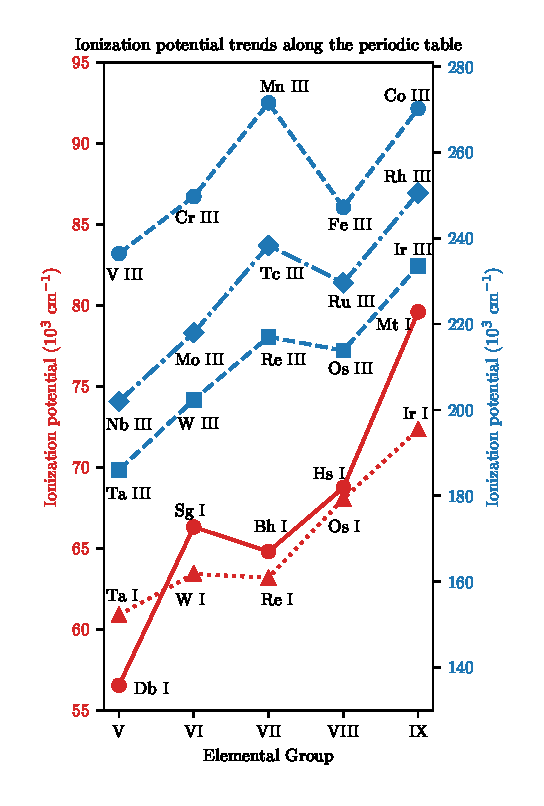
\includegraphics[scale=1.20]{./figures/Ionization_Plot.eps}
\caption[Ionization trends for open $d$-shell elements.]{Plot of ionization trends for open $d$-shell elements. The IP trend lines for the doubly ionized elements (blue) use the scale on the right and the neutral IP trend lines (red) use the left. The IPs of neutral SHEs and the doubly ionized lighter homologues Ta~\textsc{iii}, W~\textsc{iii}, Re~\textsc{iii}, Os~\textsc{iii} and Ir~\textsc{iii} were calculated using the CIPT method. All other IPs are from Ref. \cite{NIST_ASD}. \label{fig:IPPlot}}
\end{figure}

 \chapter{Atomic structure of oganesson} \label{chap:Og}
The super heavy element (SHE) oganesson ($Z=118$) was first synthesized in 2006 at Dubna \cite{OganessianOg2006} and has recently been officially named and recognized \cite{Karol2016}.  It is also the first SHE and not naturally occuring element in the group of noble elements (Group 18) where the ground state has completely filled electron $np$ shells. Like other SHEs  ($Z>100$) it is of great experimental and theoretical interest due to the high relativistic nature  which may result in exotic and anomalous chemical and physical properties \cite{Pershina2009, Schwerdtfeger2014}. In general, experimental study of SHEs is difficult  due to the short lifetimes and low production rates. Og is no exception, where the only confirmed isotope ($^{294}$Og) has a halflife of 0.7 ms \cite{OganessianOg2006}. The study of Og and other SHEs is of great interest due to their exotic characteristics such as the large dependence on relativistic effects and the possible existence of long-lived isotopes of heavy nuclei in the ``island of stability''. \\
\linebreak
 There has been a large amount of  theoretical work on the chemical and physical properties of Og with calculations of solid state and molecular properties \cite{Kullie2012, Shee2015, Nash1999, Nash2005, Peter2016}, electron affinities\cite{Pitzer1975, EliavOg1996, PershinaOg2008, Hangele2012, Goidenko2003}, and ionisation potentials and polarisabilities \cite{PershinaOg2008, Desclaux1973, Nash2005, Jerabek2018}. While some odd parity states and electric dipole (E1) transitions in the Og spectrum have been calculated in \cite{Indelicato2007} we present a more complete spectrum with both odd and even states to compare against similar states in the Rn spectrum. There has been considerable work on both relativistic and quantum electrodynamic (QED) effects \cite{Pyykko1988, Jerabek2018, Goidenko2003, Eliav2015, Indelicato2007, Thierfelder2010} in Og. In this work we included both the Breit interaction and QED radiative effects. To aid in the experimental study of Og we use  theoretical methods to further study its physical properties.  The results of this chapter were published in Ref. \cite{LDFOg2018}
\section{CIPT calculation of Rn and Og spectrum} \label{sec:CIPT}
\afterpage{
\begin{longtable}{l@{\hspace{0.5cm}}cc@{\hspace{0.5cm}}r@{\hspace{0.5cm}}r@{\hspace{0.5cm}}r@{\hspace{0.5cm}}r@{\hspace{0.5cm}}}
\caption[Comparison between experimental and theoretical (CIPT method) excitation energies in Rn I]{CIPT calculations of excitation spectrum, ionisation potential and electron affinity for Rn I with experimental results for comparison. Here $E_E$ and $E_T$ are experimental and theoretical CIPT excitation energies respectively with $\Delta = E_E - E_T$. We also present the calculated Land\'{e} $g$-factors and the energy difference between the experimental and theoretical excitation energies. (Originally published in \cite{LDFOg2018}) \label{tab:RnSpectrum}}
\endfirsthead
\multicolumn{5}{c}%
{\tablename\ \thetable\ -- \textit{Continued from previous page}} \\
\hline
\multicolumn{7}{c}{Rn I}  \\
 & State & $J$ &  \multicolumn{1}{c}{\parbox{1cm}{$E_E$\cite{NIST_ASD} \\ (cm$^{-1}$)}}  &  \multicolumn{1}{c}{\parbox{1cm}{$E_T$ \\ (cm$^{-1}$)}} &  \multicolumn{1}{c}{$g_T$} &  \multicolumn{1}{c}{\parbox{1cm}{$\Delta$ \\ (cm$^{-1}$)}}  \\
\hline
\endhead
\hline \multicolumn{5}{r}{\textit{Continued on next page}} \\
\endfoot
\endlastfoot
\toprule
\toprule
\multicolumn{7}{c}{Rn I}  \\
 & State & $J$ &  \multicolumn{1}{c}{\parbox{1cm}{$E_E$\cite{NIST_ASD} \\ (cm$^{-1}$)}}  &  \multicolumn{1}{c}{\parbox{1cm}{$E_T$ \\ (cm$^{-1}$)}} &  \multicolumn{1}{c}{$g_T$} &  \multicolumn{1}{c}{\parbox{1cm}{$\Delta$ \\ (cm$^{-1}$)}}  \\
\midrule
 \\
$6s^2 6p^6$      & $^1$S & 0 & 0    & 0    & 0    &        \\
$6s^2 6p^5 7s$ &    $^3$P$^{\rm_o}$         & 2  &  54 620  &  55 323     &  1.50     &  -703    \\
$6s^2 6p^5 7s$ &  $^1$P$^{\rm_o}$  & 1 &   55 989  & 56 607   &  1.18      &   -618    \\
$6s^2 6p^5 7p$ & $^3$S  &  1 &   66 245 & 67 171   & 1.76      &   -926     \\
$6s^2 6p^5 7p$ & $^3$D &  2 &   66 708 & 67 658  & 1.13     &   -950      \\
$6s^2 6p^5 6d$ & $^1$S$^{\rm_o}$ &   0 &  67 906  &   69 145  &  0          \\
$6s^2 6p^5 7p$ & $^3$D &  3 &   68 039  &  68 891  &  1.33      &   -852      \\
$6s^2 6p^5 7p$ & $^1$P & 1 &   68 332 &  69 313   & 1.09      & -981     \\
$6s^2 6p^5 7p$ & $^3$P &  2 &   68 790 &  69 749   & 1.37       &  -959    \\
$6s^2 6p^5 6d$ & $^3$P$^{\rm_o}$ &  1 &  68 891  & 70 002     &   1.36    & -1 111  \\
$6s^2 6p^5 7p$ & $^1$S &  0 &   69 744    &   70 800    &   0    &   -1 056      \\
$6s^2 6p^5 6d$ & $^3$F$^{\rm_o}$ &  4 &    69 798   &   70 742     &  1.25    &  -944   \\
$6s^2 6p^5 6d$ &  $^3$D$^{\rm_o}$ &  2     &   70 223   &  71 188 &   1.32    &   -965  \\
$6s^2 6p^5 6d$ & $^3$F$^{\rm_o}$ &  3 & 70 440  &  71 334 &  1.06     &    -894       \\
\multicolumn{7}{c}{Ionisation potential} \\
$6s^2 6p^5$ & $^2$P$^{\rm_o}$ & $3/2$ & 86 693 & 87 721 & 1.33 & -1 028   \\
\multicolumn{7}{c}{Electron Affinity} \\
$6s^2 6p^6 7s$ &   $^2$S & 1/2 &  & 1 868 & 2.00 &    \\
\bottomrule
\bottomrule
\end{longtable}
}
To demonstrate the accuracy of the SHE Og calculations we present the calculations of the noble analog Rn in Table~\ref{tab:RnSpectrum} to compare with experimental results. The lack of experimental $g$-factors for Rn I make it difficult to confirm the correct identification of the states and therefore we must rely solely on the order of the energy levels. We find that there is good agreement between the experimental and theoretical states with an agreement with  $\Delta \approx -900$ cm$^{-1}$ with the largest discrepancy   $\Delta \approx -1239 $~cm$^{-1}$. We expect a similar accuracy for our Og I calculations which are presented in Table~\ref{tab:OgSpectrum}. \\
\linebreak
Comparing the spectrum of Rn  to Og we see that despite the similar electronic structure (with differing principal quantum numbers) there are significant differences. The Og spectrum is much more dense than Rn  with the first excitation lying more than 20~000~cm$^{-1}$ below the equivalent excitation in Rn. This results in an odd parity state which lies in the optical region. This makes the  state a good candidate for initial experimental measurement. In the final column of Table~\ref{tab:OgSpectrum} we present the states calculated in ref.~\cite{Indelicato2007}. This work also did not present $g$-factors which made comparing states uncertain, therefore we compared them by ordering energies. For four of the states there was good agreement with our results lying within $1000$ cm$^{-1}$ however for the other states there was a large discrepancy of $>4000$ cm$^{-1}$.  \\
\linebreak
Our calculated value of the ionisation potential of Og in Table~\ref{tab:OgSpectrum} is in excellent agreement with the value calculated in Ref.~\cite{Jerabek2018} ($E_{IP}=$71~320~cm$^{-1}$) where a CCSD(T) method was used. \\
\linebreak
It has been shown that Og has a positive electron affinity which is an anomaly in the group of noble gases \cite{EliavOg1996, Goidenko2003, Eliav2015}. This is another consequence of the stabilized $8s$ orbital due to the large relativistic effects. Our calculation presented in Table \ref{tab:OgSpectrum}  confirms this with an electron affinity of 773 cm$^{-1}$ (0.095 eV) which is in good agreement with the coupled cluster value presented in \cite{Goidenko2003}. For comparison we also present the negative ion calculation for Rn I which is known to be unstable. All other negative ionic states of Og were found to be unstable.
\newpage
\afterpage{
\begin{longtable}{@{\hspace{1cm}}r@{\hspace{1cm}}r@{\hspace{0.5cm}}l@{\hspace{1cm}}cc@{\hspace{1cm}}r@{\hspace{1cm}}r@{\hspace{1cm}}r}
\caption[Theoretical excitation spectrum, ionisation potential and electron affinity for Og I]{CIPT calculations of excitation spectrum, ionisation potential and electron affinity for Og I. Here $E_T$ and $g_T$ are the theoretical CIPT excitation energies and Land\'{e} $g$-factors respectively.  (Originally published in \cite{LDFOg2018}) \label{tab:OgSpectrum}}
\endfirsthead
\multicolumn{5}{c}%
{\tablename\ \thetable\ -- \textit{Continued from previous page}} \\
\hline
\multicolumn{5}{c}{Og I} \\
 & State & $J$ & \multicolumn{1}{c}{\parbox{1cm}{$E_T$ \\ (cm$^{-1}$)}}  &  \multicolumn{1}{c}{$g_T$} & \parbox{1.5cm}{Ref. \cite{Indelicato2007}\\ (cm$^{-1}$)}  \\
\hline
\endhead
\hline \multicolumn{5}{r}{\textit{Continued on next page}} \\
\endfoot
\endlastfoot
\toprule
\toprule
\multicolumn{5}{c}{Og I} \\
 & State & $J$ & \multicolumn{1}{c}{\parbox{1cm}{$E_T$ \\ (cm$^{-1}$)}}  &  \multicolumn{1}{c}{$g_T$} & \parbox{1.5cm}{Ref. \cite{Indelicato2007}\\ (cm$^{-1}$)}  \\
\midrule
 \\
  $7s^2 7p^6$ & $^1$S & 0  &  0 & 0 & 0  \\
 $7s^2 7p^5 8s$  &  $^3$P$^{\rm_o}$  & 2 & 33 884 & 1.50 & 34 682 \\
 $7s^2 7p^5 8s$ & $^1$P$^{\rm_o}$ &  1   & 36 689    &  1.17  & 38 150   \\
 $7s^2 7p^5 8p$ & $^3$P &  1   & 49 186    &    1.60  &   \\
 $7s^2 7p^5 8p$ & $^3$D & 2    &  49 451   &   1.15    \\
 $7s^2 7p^5 8p$& $^3$D & 3    &  53 777   &    1.33 &    \\
 $7s^2 7p^5 8p$ & $^3$P &  1   & 53 881    &    1.24        \\
 $7s^2 7p^5 7d$ &  $^1$S$^{\rm_o}$ & 0    & 54 155    &  0  & 53 556    \\
$7s^2 7p^5 8p$ & $^3$P & 2     & 54 446 & 1.35 &  \\
$7s^2 7p^5 7d$ &  $^1$S$^{\rm_o}$ & 1    & 54 725    &  1.33 & 54 927 \\
$7s^2 7p^5 7d$ & $^3$F$^{\rm_o}$ & 4    &  54 938   &     1.25 & 48 474     \\
$7s^2 7p^5 7d$ & $^3$D$^{\rm_o}$ & 2    &  55 416    &    1.30 & 49 039 \\
$7s^2 7p^5 7d$ & $^3$F$^{\rm_o}$ &   3  &  55 622   &  1.06 & 49 603  \\
$7s^2 7p^5 8p$ & $^1$S & 0  &  55 729 & 0     \\
$7s^2 7p^5 7d$ & $^1$D$^{\rm_o}$ &  2   &  56 317   & 0.98 & 50 410  \\
$7s^2 7p^5 7d$ & $^5$F$^{\rm_o}$ &  3   & 56 343    &   1.25 & 50 168 \\
$7s^2 7p^5 7d$ & $^1$P$^{\rm_o}$ &  1   &  57 855   &   0.84  & 58 072  \\
\multicolumn{5}{c}{Ionisation potential} \\
$7s^2 7p^5$  & $^2$P$^{\rm_o}$ &   3/2  & 71 508    & 1.33  & 71 320\cite{Jerabek2018}    \\
\multicolumn{5}{c}{Electron Affinity} \\
 $7s^2 7p^6 8s$  & $^2$S  & 1/2    & -773$^{a}$    & 2.00  & -516 \cite{Goidenko2003}    \\
 \bottomrule
 \bottomrule
\end{longtable}
\begin{flushleft}
$^a$ Negative value indicates the state is bound.
\end{flushleft}
}

\section{Electric dipole transitions of Og} \label{sec:E1}
 While Og  follows the expected trend for elements in noble group where each consecutive element has both a smaller IP and first excitation energy. However Og has some properties which can be considered exotic even amongst the Group 18 elements. According to the calculated spectrum in Table~\ref{tab:OgSpectrum} it is the only noble element which has an allowed optical electric dipole (E1) transition ($\omega < $40~000 cm$^{-1}$) from the ground state, unlike Rn where the first odd state lies at 57~334 cm$^{-1}$. \\
 
 The E1 transition amplitudes, $D_{\text{E1}}$, between states which satisfy the conditions of opposite parity and $\Delta J \leq 1$   are calculated using the many-electron wavefunctions created in the CIPT method and the self-consistent random-phase approximation which 
 %Victor 
includes polarization of  the atomic electron core by an external electromagnetic field. The details  of the method are presented  in Ref. \cite{Dzuba2018}. \\
 
The E1 transition rate is calculated using (in atomic units),
\begin{align} \label{eq:Transitionrate}
A_{E1} = \dfrac{4}{3}\left(\alpha \omega\right)^3\dfrac{ D_{\text{E1}}^2}{2J + 1}
\end{align}
where $J$ is the angular momentum of the upper state, $\alpha$ is the fine structure constant and $\omega$ is the frequency of the transition in atomic units. The transition amplitudes and transition rates for the allowed E1 transitions in Og are presented in Table~\ref{tab:E1_transitions}. In ref.~\cite{Indelicato2007} the major E1 transition rates were also calculated with a MCDF approach, these are included for comparison Table~\ref{tab:E1_transitions}. \\
\linebreak
\begin{table}[h]
\centering
\caption[Comparison of E1 transition rates between experimental and CIPT values for Kr I and Xe I]{Comparison of E1 transition rates between experimental and CIPT values for Kr I and Xe I. Here $D_{E1}$ is the transition amplitude in atomic units and $A_{E1}$ is the transition rate. \label{tab:E1_comp}}
\begin{tabular}{c@{\hspace{0.5cm}}c@{\hspace{1cm}}c@{\hspace{0.5cm}}c@{\hspace{0.5cm}}c}
\toprule
\toprule
State & $E_{\text{Exp}}$ & $D_{\text{E1}}$ & $A_{\text{E1, CIPT}}$ & $A_{\text{E1,Exp}}$  \\
&  (cm$^{-1}$) & (a.u.) &  ($\times 10^6$ s$^{-1}$) &  ($\times 10^6$ s$^{-1}$)  \\
\hline
\multicolumn{5}{c}{Kr I} \\
$^1$P$_1^{\rm_o}$ & 80 916 & 0.94  & 314  & 312\cite{Fuhr1996} \\
 $^3$P$_1^{\rm_o}$ & 85 846 & 0.87  & 320  & 316\cite{Fuhr1996}   \\
 \multicolumn{5}{c}{Xe I} \\
 $^1$P$_1^{\rm_o}$ & 68 045 & 1.18  & 295  & 273 \cite{Morton2000} \\
 $^3$P$_1^{\rm_o}$ & 77 185 & 0.98  & 298  & 253 \cite{Morton2000}  \\
\bottomrule
\bottomrule
\end{tabular}
\end{table}

We calculated the  rates of the $(n+1)s \rightarrow np$ transitions in lighter neutral noble elements Kr and Xe  and compared them to experimental values, these are presented in Table \ref{tab:E1_comp}. The experimental uncertainties are approximately $2\%$ for Xe I transitions \cite{Morton2000} and $~10$-$25\%$ for Kr I transitions\cite{Fuhr1996}. Comparing our calculated values to the experimental values in Table \ref{tab:E1_comp} we see the accuracy for these transitions is from 0.6\% to 17.7\%. We used the experimental energies to calculate the transitions rates of Kr I and Xe I using (\ref{eq:Transitionrate}) and since the uncertainty in the experimental energies are negligible the uncertainty in our calculations compared to experimental results in Table \ref{tab:E1_comp} is equivalent to the uncertainty in the square of the calculated transition amplitude $D_{E1}^2$. For our calculation of the Og I transition rates we needed to take into account the non-negligible uncertainty in the energies of our CIPT calculations.  Therefore assuming an accuracy of 18\% for $D_{E1}^2$ and an uncertainty of 3\% in the CIPT energy ($\left|\Delta\right| \approx 1000$~cm$^{-1}$) we expect a transition rate accuracy of 20\% for the $8s \rightarrow 7p$ optical transition ($\omega = 36~689$~cm$^{-1}$) of Og I in Table \ref{tab:E1_transitions}.  \\

\begin{table}[h]
\centering
\caption[Theoretical electric dipole transition amplitudes and rates of Og I]{Electric dipole transition amplitudes of Og I from the ground state $^1$S$_0$ to the excited states of odd parity and angular momenta $J=1$. Here $D_{E1}$ is the transition amplitude in atomic units and $A_{E1}$ is the transition rate. We include results of MCDF calculations from ref. \cite{Indelicato2007} for comparision. There is significant disagreement for the third transition however there is another transition in \cite{Indelicato2007} which has a rate ($986 \times 10^{6}$ s$^{-1}$) close to our calculated value. So, the disagreement  may be the result of a misprint in \cite{Indelicato2007}. (Originally published in \cite{LDFOg2018}).\label{tab:E1_transitions}}
\begin{tabular}{c@{\hspace{0.5cm}}c@{\hspace{1cm}}c@{\hspace{0.5cm}}c@{\hspace{0.5cm}}c}
\toprule
\toprule
State & $E_{\text{CIPT}}$ & $D_{\text{E1}}$ & $A_{\text{E1, CIPT}}$ & $A_{\text{E1,MCDF}}$ \cite{Indelicato2007}  \\
&  (cm$^{-1}$) & (a.u.) &  ($\times 10^6$ s$^{-1}$) &  ($\times 10^6$ s$^{-1}$)  \\
\hline
$^1$P$_1^{\rm_o}$ & 36 689 & 2.09 & 145 & 204\\
 $^1$S$_1^{\rm_o}$ & 54 725 & 0.727 & 58.4 & 55.3  \\
 $^1$P$_1^{\rm_o}$ & 57 855 & -2.67 & 936 & 9.9, 986* \\
\bottomrule
\bottomrule
\end{tabular}
\end{table}
Only the first transition in Table \ref{tab:E1_transitions} lies in the optical region and therefore it has the highest likelihood of being measured first. The large rate of the transition $^1$S$_0$~$\rightarrow$~$^1$P$_1^{\rm_o}$ is also promising for experimental measurement. 

\section{Electron density of  Og} \label{sec:Relativistic}
The electron density of SHE gives insight into the effectiveness of the codes.
\begin{figure} 
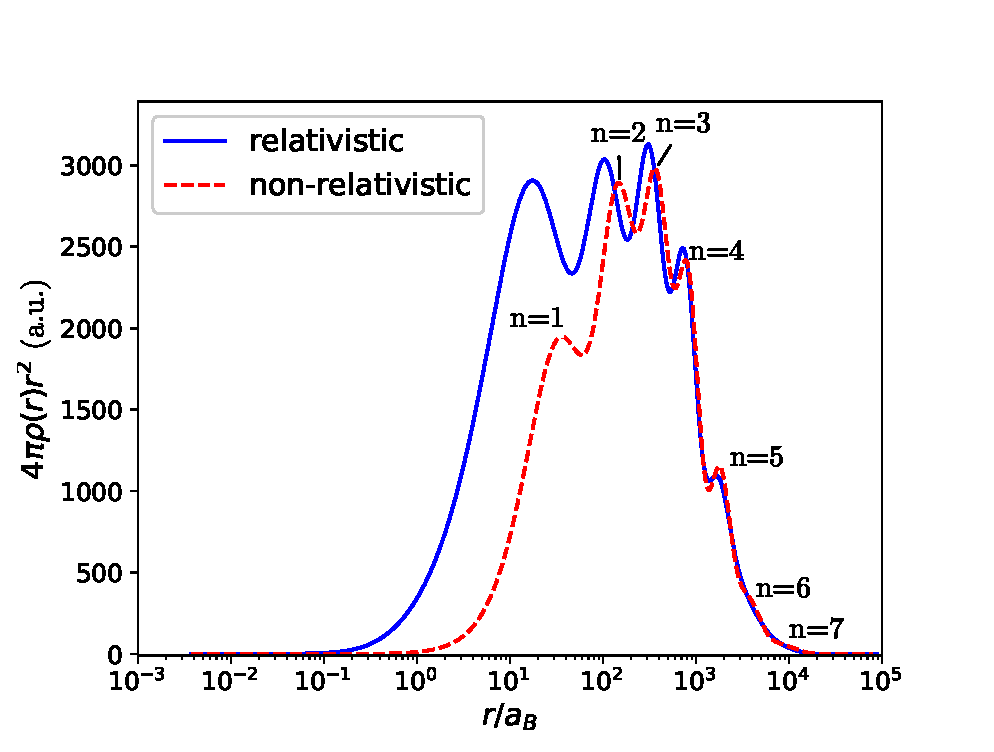
\includegraphics[scale=0.8]{./figures/Ogplot.eps}
\caption[Relativistic and non-relativistic radial electron density of Og I.]{Radial electron density, $4\pi\rho(r)r^2$ plot for Og I in both relativistic and non-relativistic approximations. The solid blue line and the dashed red line are non-relativistic and relativistic approximations respectively. The principle quantum peaks have been labeled for the non-relativic plot. (Originally published in \cite{LDFOg2018})\label{Og_plot}}
\end{figure}
\begin{figure}
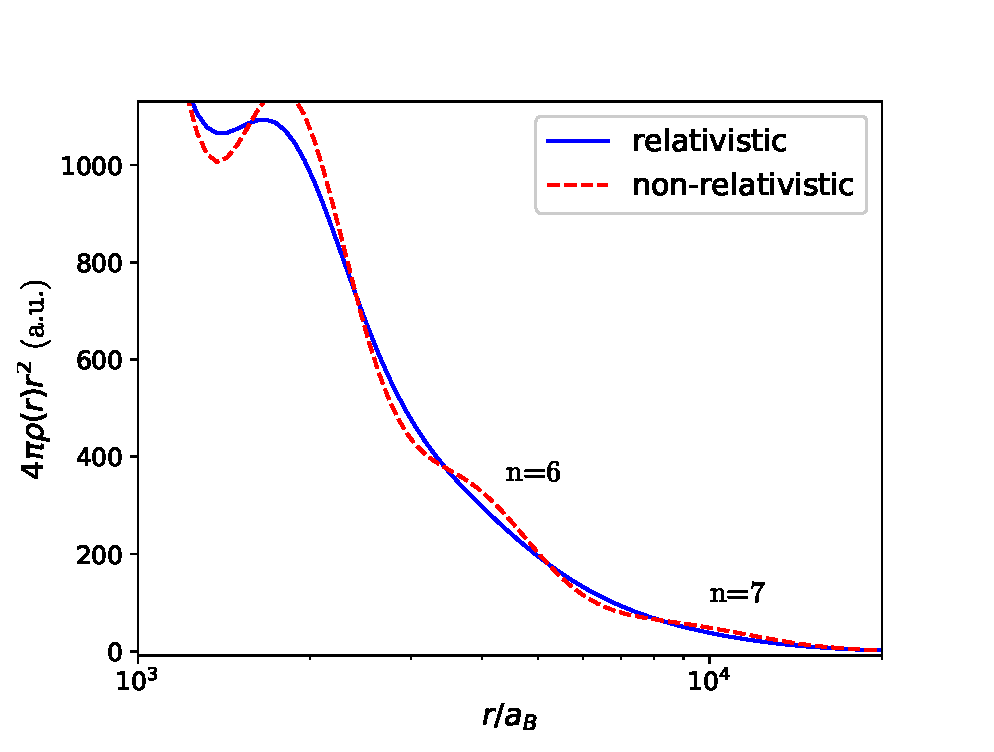
\includegraphics[scale=0.8]{./figures/Ogplot_zoom.eps}
\caption{Lower right section of  Figure~\ref{Og_plot}.\label{Og_plot_zoom}}
\end{figure}
It has been shown in Ref. \cite{Jerabek2018} using fermion localization that the electron density of Og is smoother than other group 18 analogues which have distinct atomic shells . The cause of this is the large relativistic effects in SHE which effectively smear out the shells into a smoother electron density (the same was shown for the nucleon density). The relativistic effects can also be seen by looking at the radial electron densities with relativistic and non-relativistic approximations. The Hartree-Fock radial electron density for Og is plotted on a logarithmic scale in Figure~\ref{Og_plot} in both the relativistic and non-relativistic approximations. There are a total of 7 peaks in the radial densities corresponding to the principle quantum numbers $n$ where lower shells have distinct peaks in both the relativistic and non-relativistic approximations. As expected, in the relativistic approximation the inner shells ($n=1,2,3$) shift closer to the nucleus however higher shells are relatively unaffected ($n \geq 4$). This results in a similar density profile for the electrons a large distance away from the nucleus. \\
\linebreak
In Figure~\ref{Og_plot_zoom} we plot the tail of the density function in Figure~\ref{Og_plot}. Here we see that, while spread out, the principle shell peaks still exist in the non-relativistic approximation. However in the relativistic approximation the density has been smoothed out to such a degree that there are no discernible peaks. This supports the results in ref.~\cite{Jerabek2018} where they calculated the electron shell structure of Og I and found that it disappears for external shells due to the high relativistic effects. This can be explained as the large spin-orbit splitting doubles the number of sub-shells which overlap making the overall distribution smooth.\\

\chapter{Conclusion} \label{chap:P2Conc}
The study of elements at the extremes of the periodic table has been a cornerstone of science for centuries. Currently the progress of this filed is experimentally limited due to the large cost of these facilities and and the low short lifetimes and low production rates for SHEs. With the sparse experimental results of spectroscopic properties of these elements, physicists must look towards theoretical many-body models to study these techniques. In this thesis I have presented results from many-body treatment of the electronic structure of some of these SHEs. Specifically, I have presented the low lying energy spectrum of Db, Sg, Bh, Hs, Mt and Og elements along with the strong optical E1 transitions and associated isotope shifts from the CIPT method. \\
\linebreak
In studying these atoms I also highlighted the strong relativistic effects and their effect on the electronic shells. The spectra of all the elements displayed the direct and indirect effects of the stabilization and contraction of the $7s$ orbital and the resultant destabilization of the $6d$ orbital. This effect primarily manifested in the systematic lowering of the odd parity spectrum for all the open $6d$-shell SHE when compared to their lighter analog. Also, this low energy, odd parity spectrum is dominated by states with valence configuration $6d^{n}7s^27p$ where $n=2-6$ for elements Db-Mt. The other relativistic effect we observed was the large fine structure splitting of the $6d$ shell. This manifested in the violation of Hund's rule, where the $6d_{3/2}$ shell was filled separately to the $6d_{5/2}$ shell. To our understanding, this is the first observation of the fine structure splitting of the $6d$ shell.\\
\linebreak
With recent evidence supporting the existence of these metastable nuclei in the universe \cite{Alexandrov2019} the search for the island of stability in astrophysical data is even more promising. The calculated isotope shifts presented in this thesis may help translate measured transitions of neutron deficient isotopes in laboratories to their metastable isotopes. However future progress is limited by the experimental measurements of these neutron deficient isotopes and transitions and current experimental methods are dependent on targeted spectroscopic scans and highly accurate predictions of these states are needed which were supplied in this work.\\
\linebreak
Possible future work on the isotope shift calculations is the consideration of more exotic nuclear density profile and these may affect the isotope shift. The existence of a central depression in the nuclear density or even the extreme case of toriodal distributions of nuclear matter are expected for isotopes of the these SHEs \cite{FD2019}. Consideration of these differing nuclear profiles in the atomic calculations using the CIPT method are an important approach to take as currently only a simple Fermi distribution is considered. These calculations could reveal interesting properties of the atomic structure of SHEs and even test the current limits of the periodic table.\\
\linebreak
These initial calculations of the open $6d-$shell SHE should set a good foundation for future theoretical and experimental study of the exotic elements. 
\appendix



\chapter{Nilsson Orbitals} \label{chap:Nilsson}
In Chapter \ref{chap:Deformed} I discussed the Nilsson model for deformed nuclei. In this Appendix I present the Nilsson values for each nucleons and the open shell configurations for the nuclei of interest. The properties of all the nuclei of interest were calculated using the Nilsson energy level plots in A. Bohr's and B. R. Mottelson's Nuclear Structure Volume~II \cite{BohrMottVol2} which are reproduced in Figure~\ref{fig:NilssonPlots}. 
\begin{figure}
\centering
\begin{subfigure}[b]{0.45\textwidth}
    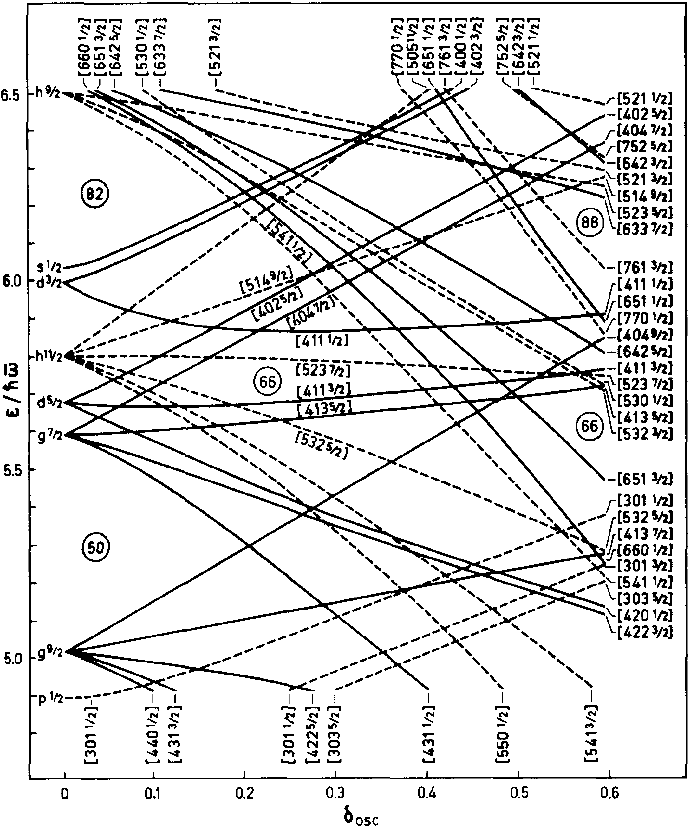
\includegraphics[width=\textwidth]{./figures/Nilsson/proton_deformed50.png}
    \caption{$50<Z<82$}
\end{subfigure}	
\quad
\begin{subfigure}[b]{0.45\textwidth}
    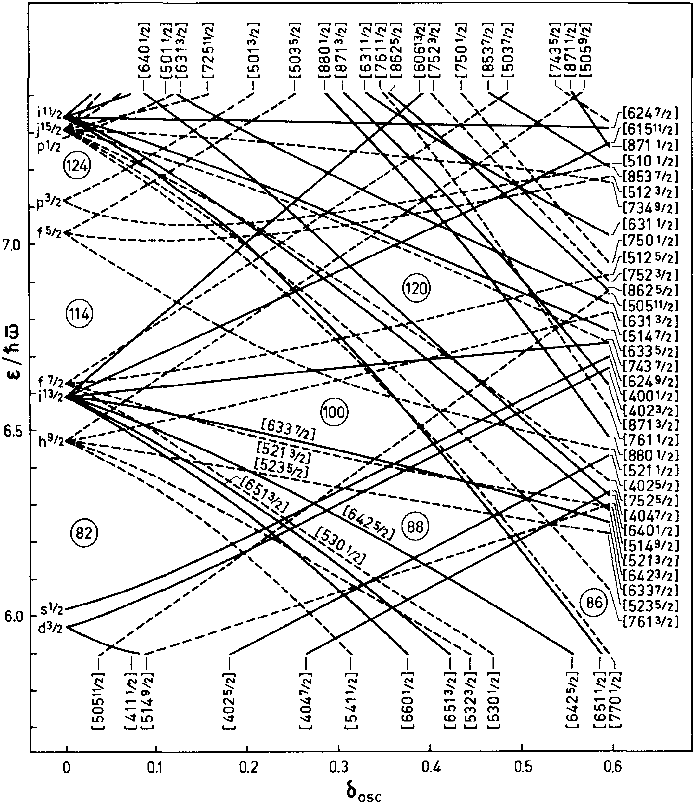
\includegraphics[width=\textwidth]{./figures/Nilsson/proton_deformed82.png}
    \caption{$Z>82$}
\end{subfigure}
\\
\begin{subfigure}[b]{0.48\textwidth}
    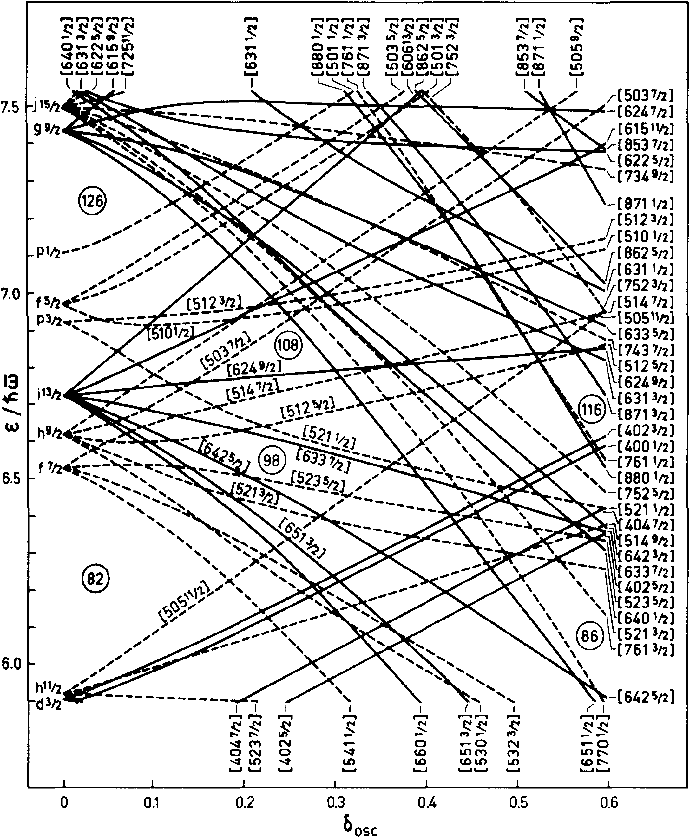
\includegraphics[width=\textwidth]{./figures/Nilsson/neutron_deformed82.png}
    \caption{$82<N<126$}
\end{subfigure}	
\quad
\begin{subfigure}[b]{0.48\textwidth}
    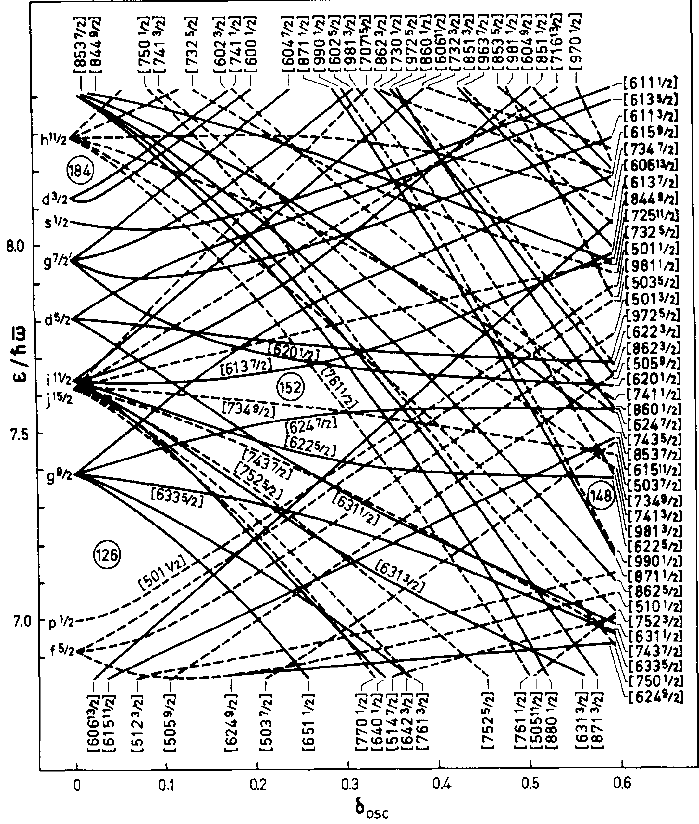
\includegraphics[width=\textwidth]{./figures/Nilsson/neutron_deformed126.png}
    \caption{$N>126$}
\end{subfigure}
\caption{Nilsson energy diagrams for both protons and neutrons for prolate deformed nuclei. Here $\delta_{\text{osc}}$ is a degree of deformation. The numbers in circles represent the magic numbers in the spherical limit. These figures have been taken from A. Bohr B. R. Mottelson, Nuclear Structure Vol. 2 \cite{BohrMottVol2}. \label{fig:NilssonPlots}}

\end{figure}
\section{Quantum numbers for Nilsson orbitals}
To calculate the tensor properties of nuclei discussed in Chapters~\ref{chap:WQM} and \ref{chap:MQM} the quantum numbers of the orbitals are required. The nucleon configuration of nuclei can be divided into completely filled major nuclear shells ($N$) and unfilled shells. The Nilsson numbers of interest for the tensor properties calculated in this thesis are presented in Table~\ref{table:FullShellNz} for complete shells and Table~\ref{table:NilssonNucleon} for individual nucleons.

\begin{table} 
\centering
\caption[Collective Nilsson for for major shells.]{This table presents the collective Nilsson values $\sum 2n_z + 1$ and $\sum N - n_z + 1$ for major shells $N$. This is identical for both protons and neutrons. \label{table:FullShellNz}}
\begin{tabular}{c|c}
\toprule
\toprule
Filled $N$ Shell & $\sum 2n_z + 1 = \sum N - n_z + 1$ \\ [2pt]
\midrule
0 & 2\\
1 & 10\\
2 & 28\\
3 & 60\\
4 & 110\\
5 & 182 \\
\bottomrule
\bottomrule
\end{tabular}
\end{table}
\afterpage{
%\begin{table}[htbp]
%\centering
\begin{longtable}{l@{\hspace{1cm}}r@{\hspace{1cm}}c@{\hspace{1cm}}c@{\hspace{1cm}}c}
\caption{Nilsson values, $2n_z + 1$, $N - n_z + 1$ and $\Sigma\Lambda$ for individual nucleons \label{table:NilssonNucleon}}\\
\endfirsthead
\multicolumn{5}{c}%
{\tablename\ \thetable\ -- \textit{Continued from previous page}} \\
\hline
$l_m$      & $\Omega[Nn_z\Lambda]$ & $2n_z + 1$ & $N - n_z + 1$ & $\Sigma\Lambda$ \\
\hline
\endhead
\hline \multicolumn{5}{r}{\textit{Continued on next page}} \\
\endfoot
\endlastfoot
\toprule
\toprule
$l_m$      & $\Omega[Nn_z\Lambda]$ & $2n_z + 1$ & $N - n_z + 1$ & $\Sigma\Lambda$ \\
\midrule
\multicolumn{5}{l}{$N=0$} \\
1$s_{1/2}$ & $1/2[000]$            & 1          & 1             & 0            \\
\multicolumn{5}{l}{$N=1$} \\
1$p_{3/2}$ & $1/2[110]$            & 3          & 1             & 0          \\
1$p_{3/2}$ & $3/2[101]$            & 1          & 2             & 1/2           \\
1$p_{1/2}$ & $1/2[101]$            & 1          & 2             & -1/2          \\
\multicolumn{5}{l}{$N=2$} \\
1$d_{5/2}$ & $1/2[220]$            & 5          & 1             & 0        \\
1$d_{5/2}$ & $3/2[211]$            & 3          & 2             & 1/2          \\
1$d_{5/2}$ & $5/2[202]$            & 1          & 3             & 1             \\
2$s_{1/2}$ & $1/2[211]$            & 3          & 2             & -1/2           \\
1$d_{3/2}$ & $1/2[200]$            & 1          & 3             & 0             \\
1$d_{3/2}$ & $3/2[202]$            & 1          & 3             & -1            \\
\multicolumn{5}{l}{$N=3$} \\
1$f_{7/2}$ & $1/2[330]$            & 7          & 1             & 0             \\
1$f_{7/2}$ & $3/2[321]$            & 5          & 2             & 1/2               \\
1$f_{7/2}$ & $5/2[312]$            & 3          & 3             & 1             \\
1$f_{7/2}$ & $7/2[303]$            & 1          & 4             & 3/2               \\
2$p_{3/2}$ & $1/2[321]$            & 5          & 2             & -1/2              \\
2$p_{3/2}$ & $3/2[312]$            & 3          & 3             & -1              \\
1$f_{5/2}$ & $1/2[310]$            & 3          & 3             & 0              \\
1$f_{5/2}$ & $3/2[301]$            & 1          & 4             & 1/2               \\
1$f_{5/2}$ & $5/2[303]$            & 1          & 4             & -3/2               \\
2$p_{1/2}$ & $1/2[301]$            & 1          & 4             & -1/2               \\
\multicolumn{5}{l}{$N=4$} \\
1$g_{9/2}$ & $1/2[440]$            & 9          & 1             & 0               \\
1$g_{9/2}$ & $3/2[431]$            & 7          & 2             & 1/2               \\
1$g_{9/2}$ & $5/2[422]$            & 5          & 3             & 1               \\
1$g_{9/2}$ & $7/2[413]$            & 3          & 4             & 3/2               \\
1$g_{9/2}$ & $9/2[404]$            & 1          & 5             & 2              \\
1$g_{7/2}$ & $1/2[431]$            & 7          & 2             & -1/2             \\
1$g_{7/2}$ & $3/2[422]$            & 5          & 3             & -1             \\
1$g_{7/2}$ & $5/2[413]$            & 3          & 4             & -3/2            \\ 
1$g_{7/2}$ & $7/2[404]$            & 1          & 5             & -2              \\
2$d_{5/2}$ & $1/2[420]$            & 5          & 3             & 0              \\
2$d_{5/2}$ & $3/2[411]$            & 3          & 4             & 1/2            \\
2$d_{5/2}$ & $5/2[402]$            & 1          & 5             & 1    \\
2$d_{3/2}$ & $1/2[411]$            & 3          & 4             & -1/2               \\
2$d_{3/2}$ & $3/2[402]$            & 1          & 5             & -1               \\
3$s_{1/2}$ & $1/2[400]$            & 1          & 5             & 1/2           \\
\multicolumn{5}{l}{$N=5$} \\
1$h_{11/2}$ & $1/2[550]$            & 11         & 1             & 0             \\
1$h_{11/2}$ & $3/2[541]$            & 9          & 2             & 1/2               \\
1$h_{11/2}$ & $5/2[532]$            & 7          & 3             & 1           \\
1$h_{11/2}$ & $7/2[523]$            & 5          & 4             & 3/2         \\
1$h_{11/2}$ & $9/2[514]$            & 3          & 5             & 2         \\
1$h_{11/2}$ & $11/2[505]$           & 1          & 6             & 5/2            \\
1$h_{9/2}$ & $1/2[541]$             & 9          & 2             & -1/2          \\
1$h_{9/2}$ & $3/2[532]$             & 7          & 3             & -1        \\
1$h_{9/2}$ & $5/2[523]$             & 5          & 4             & -3/2            \\
1$h_{9/2}$ & $7/2[514]$             & 3          & 5             & -2         \\
1$h_{9/2}$ & $9/2[505]$             & 1          & 6             & -5/2           \\
2$f_{7/2}$ & $1/2[530]$             & 7          & 3             & 0             \\
2$f_{7/2}$ & $3/2[521]$             & 5          & 4             & 1/2               \\
2$f_{7/2}$ & $5/2[512]$             & 3          & 5             & 1           \\
2$f_{7/2}$ & $7/2[503]$             & 1          & 6             & 3/2           \\
3$p_{3/2}$ & $1/2[521]$             & 5          & 4             & -1/2           \\
3$p_{3/2}$ & $3/2[512]$             & 3          & 5             & -1            \\
2$f_{5/2}$ & $1/2[510]$             & 3          & 5             & 0         \\
2$f_{5/2}$ & $3/2[501]$             & 1          & 6             & 1/2           \\
2$f_{5/2}$ & $5/2[503]$             & 1          & 6             & -3/2           \\
3$p_{1/2}$ & $1/2[501]$             & 1          & 6             & -1/2            \\
\multicolumn{5}{l}{$N=6$} \\
1$i_{13/2}$ & $1/2[660]$            & 13         & 1             & 0            \\
1$i_{13/2}$ & $3/2[651]$            & 11         & 2             & 1/2        \\
1$i_{13/2}$ & $5/2[642]$            & 9          & 3             & 2           \\
1$i_{13/2}$ & $7/2[633]$            & 7          & 4             & 3/2       \\
1$i_{13/2}$ & $9/2[624]$            & 5          & 5             & 2      \\
1$i_{13/2}$ & $11/2[615]$           & 3          & 6             & 5/2       \\
1$i_{13/2}$ & $13/2[606]$           & 1          & 7             & 3        \\
2$g_{9/2}$  & $1/2[651]$            & 11         & 2             & -1/2         \\
2$g_{9/2}$  & $3/2[642]$            & 9          & 3             & -1     \\
2$g_{9/2}$  & $5/2[633]$            & 7          & 4             & -3/2      \\
2$g_{9/2}$  & $7/2[624]$            & 5          & 5             & -2        \\
2$g_{9/2}$  & $9/2[615]$            & 3          & 6             & -5/2     \\
1$i_{11/2}$ & $1/2[640]$            & 9          & 3             & 0       \\
1$i_{11/2}$ & $3/2[631]$            & 7          & 4             & 1/2    \\
1$i_{11/2}$ & $5/2[622]$            & 5          & 5             & 1       \\
1$i_{11/2}$ & $7/2[613]$            & 3          & 6             & 3/2      \\
1$i_{11/2}$ & $9/2[604]$            & 1          & 7             & 2            \\
1$i_{11/2}$ & $11/2[606]$           & 1          & 7             & -3          \\
\vdots      & \vdots                & \vdots     & \vdots        & \vdots           \\
\multicolumn{5}{l}{$N=7$} \\
1$j_{15/2}$ & $1/2[770]$            & 15         & 1             & 0            \\
1$j_{15/2}$ & $3/2[761]$            & 13         & 2             & 1/2         \\
1$j_{15/2}$ & $5/2[752]$            & 11         & 3             & 1          \\
1$j_{15/2}$ & $7/2[743]$            & 9          & 4             & 3/2         \\
1$j_{15/2}$ & $9/2[734]$            & 7          & 5             & 2              \\
1$j_{15/2}$ & $11/2[725]$            & 5          & 6             & 5/2           \\
1$j_{15/2}$ & $13/2[716]$            & 3          & 7             & 3         \\
1$j_{15/2}$ & $15/2[707]$            & 1          & 8             & 7/2         \\
\vdots      & \vdots                & \vdots     & \vdots        & \vdots           \\
\bottomrule
\bottomrule
\end{longtable}
}
\section{Filled and Unfilled shells of Nuclei}
Below is a table of the filled and unfilled $N$ shells of the deformed nuclei of interest. For Eu isotopes there are two applicable deformations, large or small. Due to the relative electric quadrupole moments of the two isotopes (Ref.~\cite{Stone2005}) we assumed a large deformation for $^{153}$Eu and small deformation for $^{151}$Eu.
\newpage
\begin{longtable}{cll}
\caption{Population of protons and neutrons in deformed nuclei. The coloured numbers represent the unpaired nucleon for each nucleus.}\\
\endfirsthead
\multicolumn{3}{c}%
{\tablename\ \thetable\ -- \textit{Continued from previous page}} \\
\toprule
\toprule
Nuclei      & Protons & Neutrons \\
\midrule
\endhead
\hline \multicolumn{3}{r}{\textit{Continued on next page}} \\
\endfoot
\endlastfoot
\toprule
\toprule
Nuclei  &  Protons & Neutrons \\
\midrule
$^{9}$Be                          
    &  \pbox{20cm}{Filled Shells: N/A \\
    $1s_{1/2}$: $\pm 1/2$ \\
    $1p_{3/2}$: $\pm 1/2$}              
    &  \pbox{20cm}{Filled Shells: N/A \\
    $1s_{1/2}$: $\pm 1/2$ \\
    $1p_{3/2}$: $\pm 1/2, \textcolor{BrickRed}{3/2}$}\\
\midrule
$^{21}$Ne         
    &  \pbox{20cm}{Filled Shells: N/A \\
    $1s_{1/2}$: $\pm 1/2$ \\
    $1p_{3/2}$: $\pm 1/2$, $\pm 3/2$ \\
    $1p_{1/2}$: $\pm 1/2$ \\
    $1d_{5/2}$: $\pm 1/2$}              
    &  \pbox{20cm}{Filled Shells: N/A \\
    $1s_{1/2}$: $\pm 1/2$ \\
    $1p_{3/2}$: $\pm 1/2$, $\pm 3/2$ \\
    $1p_{1/2}$: $\pm 1/2$ \\
    $1d_{5/2}$: $\pm 1/2$, $\textcolor{BrickRed}{3/2}$}\\
\midrule
$^{27}$Al         
    &  \pbox{20cm}{Filled Shells: N/A \\
    $1s_{1/2}$: $\pm 1/2$ \\
    $1p_{3/2}$: $\pm 1/2$, $\pm 3/2$ \\
    $1p_{1/2}$: $\pm 1/2$ \\
    $1d_{5/2}$: $\pm 1/2$, $\pm 3/2$, $\textcolor{RoyalBlue}{5/2}$}              
    &  \pbox{20cm}{Filled Shells: N/A \\
    $1s_{1/2}$: $\pm 1/2$ \\
    $1p_{3/2}$: $\pm 1/2$, $\pm 3/2$ \\
    $1p_{1/2}$: $\pm 1/2$ \\
    $1d_{5/2}$: $\pm 1/2$, $\pm 3/2$, $\pm 5/2$}\\
\midrule
$^{163}$Dy 
    &  \pbox{20cm}{Filled Shells: N = 0, 1, 2, 3 \\
    $1g_{9/2}$: Full Shell \\
    $1g_{7/2}$: $\pm 1/2$, $\pm 3/2$, $\pm 5/2$ \\
    $2d_{5/2}$: $\pm 1/2$, $\pm 3/2$ \\
    $1h_{11/2}$:$\pm 1/2$, $\pm 3/2$, $\pm 5/2$}              
    &  \pbox{20cm}{Filled Shells: N = 0, 1, 2, 3, 4 \\
    $1h_{11/2}$: Full Shell \\
    $2f_{7/2}$: $\pm 1/2$, $\pm 3/2$, $\textcolor{BrickRed}{5/2}$ \\
    $1h_{9/2}$: $\pm 1/2$, $\pm 3/2$ \\
    $1i_{13/2}$: $\pm 1/2$, $\pm 3/2$} \\
\midrule
$^{173}$Yb 
    &  \pbox{20cm}{Filled Shells: N = 0, 1, 2, 3 \\
    $1g_{9/2}$: Full Shell \\
    $1g_{7/2}$: $\pm 1/2$, $\pm 3/2$, $\pm 5/2$ \\
    $2d_{5/2}$: $\pm 1/2$, $\pm 3/2$ \\
    $1h_{11/2}$:$\pm 1/2$, $\pm 3/2$, $\pm 5/2$, $\pm 7/2$ \\
    $2d_{3/2}$: $\pm 1/2$}              
    &  \pbox{20cm}{Filled Shells: N = 0, 1, 2, 3, 4 \\
    $1h_{11/2}$: Full Shell \\
    $2f_{7/2}$: $\pm 1/2$, $\pm 3/2$, $\pm 5/2$ \\
    $1h_{9/2}$: $\pm 1/2$, $\pm 3/2$, $\textcolor{BrickRed}{5/2}$ \\
    $1i_{13/2}$:$\pm 1/2$, $\pm 3/2$, $\pm 5/2$, $\pm 7/2$ \\
    $3p_{3/2}$: $\pm 1/2$} \\
\midrule
$^{177}$Hf 
    &  \pbox{20cm}{Filled Shells: N = 0, 1, 2, 3 \\
    $1g_{9/2}$: Full Shell \\
    $1g_{7/2}$: Full Shell \\
    $2d_{5/2}$: $\pm 1/2$, $\pm 3/2$, $\pm 5/2$ \\
    $1h_{11/2}$:$\pm 1/2$, $\pm 3/2$, $\pm 5/2$, $\pm 7/2$}              
    &  \pbox{20cm}{Filled Shells: N = 0, 1, 2, 3, 4 \\
    $1h_{11/2}$: Full Shell \\
    $2f_{7/2}$: Full Shell \\
    $1h_{9/2}$: $\pm 1/2$, $\pm 3/2$, $\textcolor{BrickRed}{5/2}$ \\
    $1i_{13/2}$:$\pm 1/2$, $\pm 3/2$, $\pm 5/2$, $\pm 7/2$} \\
\midrule
$^{179}$Hf 
    &  \pbox{20cm}{Filled Shells: N = 0, 1, 2, 3 \\
    $1g_{9/2}$: Full Shell \\
    $1g_{7/2}$: Full Shell \\
    $2d_{5/2}$: $\pm 1/2$, $\pm 3/2$, $\pm 5/2$ \\
    $1h_{11/2}$:$\pm 1/2$, $\pm 3/2$, $\pm 5/2$, $\pm 7/2$}          
    &  \pbox{20cm}{Filled Shells: N = 0, 1, 2, 3, 4 \\
    $1h_{11/2}$: Full Shell \\
    $2f_{7/2}$: Full Shell \\
    $1h_{9/2}$: $\pm 1/2$, $\pm 3/2$, $\pm 5/2$ \\
    $1i_{13/2}$:$\pm 1/2$, $\pm 3/2$, $\pm 5/2$, $\pm 7/2$, $\textcolor{BrickRed}{9/2}$} \\
\midrule
$^{181}$Ta 
    &  \pbox{20cm}{Filled Shells: N = 0, 1, 2, 3 \\
    $1g_{9/2}$: Full Shell \\
    $1g_{7/2}$: $\pm 1/2$, $\pm 3/2$, $\pm 5/2$, $\textcolor{RoyalBlue}{7/2}$ \\
    $2d_{5/2}$: $\pm 1/2$, $\pm 3/2$ \\
    $1h_{11/2}$:$\pm 1/2$, $\pm 3/2$, $\pm 5/2$, $\pm 7/2$ \\
    $2d_{3/2}$: $\pm 1/2$ \\
    $1h_{9/2}$: $\pm 1/2$}              
    &  \pbox{20cm}{Filled Shells: N = 0, 1, 2, 3, 4 \\
    $1h_{11/2}$: Full Shell \\
    $2f_{7/2}$: Full Shell \\
    $1h_{9/2}$: $\pm 1/2$, $\pm 3/2$, $\pm {5/2}$ \\
    $1i_{13/2}$:$\pm 1/2$, $\pm 3/2$, $\pm 5/2$, $\pm 7/2$ \\
    $1p_{3/2}$: $\pm 1/2$ \\
    $1g_{9/2}$: $\pm 1/2$} \\
\midrule
$^{201}$Hg 
    &  \pbox{20cm}{Filled Shells: N = 0, 1, 2, 3 \\
    $1g_{9/2}$: Full Shell \\
    $1g_{7/2}$: Full Shell \\
    $2d_{5/2}$: Full Shell \\
    $1h_{11/2}$: Full Shell \\
    $2d_{3/2}$: Full Shell}              
    &  \pbox{20cm}{Filled Shells: N = 0, 1, 2, 3, 4 \\
    $1h_{11/2}$: Full Shell \\
    $2f_{7/2}$: Full Shell \\
    $1h_{9/2}$: Full Shell \\
    $1i_{13/2}$: Full Shell \\
    $1p_{3/2}$: Full Shell \\
    $1f_{5/2}$: $\pm 1/2$, \textcolor{BrickRed}{3/2}} \\
\midrule
$^{229}$Th 
    &  \pbox{20cm}{Filled Shells: N = 0, 1, 2, 3, 4 \\
    $1h_{11/2}$: Full Shell \\
    $1h_{9/2}$: $\pm 1/2$, $\pm 3/2$ \\
    $1i_{13/2}$: $\pm 1/2$, $\pm 3/2$}              
    &  \pbox{20cm}{Filled Shells: N = 0, 1, 2, 3, 4, 5 \\
    $1i_{13/2}$: Full Shell \\
    $1g_{9/2}$: $\pm 1/2$, $\pm 3/2$, $\textcolor{BrickRed}{5/2}$ \\
    $1i_{11/2}$: $\pm 1/2$, $\pm 3/2$ \\
    $1j_{15/2}$: $\pm 1/2$, $\pm 3/2$} \\
\midrule
$^{151}$Eu 
    &  \pbox{20cm}{Filled Shells: N = 0, 1, 2, 3 \\
    $1g_{9/2}$: Full Shell \\
    $1g_{7/2}$: Full Shell \\
    $2d_{5/2}$: $\pm 1/2$, $\pm 3/2$, $\textcolor{RoyalBlue}{5/2}$ }          
    &  \pbox{20cm}{Filled Shells: N = 0, 1, 2, 3, 4 \\
    $1h_{11/2}$: Full Shell \\
    $2f_{7/2}$:$\pm 1/2$, $\pm 3/2$, $\pm 5/2$} \\
\midrule
$^{153}$Eu 
    &  \pbox{20cm}{Filled Shells: N = 0, 1, 2, 3 \\
    $1g_{9/2}$: Full Shell \\
    $1g_{7/2}$: $\pm 1/2$, $\pm 3/2$, $\textcolor{RoyalBlue}{5/2}$ \\
    $2d_{5/2}$: $\pm 1/2$ \\ 
    $1h_{11/2}$:$\pm 1/2$, $\pm 3/2$, $\pm 5/2$}          
    &  \pbox{20cm}{Filled Shells: N = 0, 1, 2, 3, 4 \\
    $1h_{11/2}$: Full Shell \\
    $2f_{7/2}$:$\pm 1/2$, $\pm 3/2$ \\
    $1h_{9/2}$: $\pm 1/2$ \\
    $1i_{13/2}$: $\pm 1/2$} \\
\midrule
$^{167}$Er           
    &  \pbox{20cm}{Filled Shells: N = 0, 1, 2, 3 \\
    $1g_{9/2}$: Full Shell \\
    $1g_{7/2}$: $\pm 1/2$, $\pm 3/2$, $\pm 5/2$\\
    $2d_{5/2}$: $\pm 1/2$, $\pm 3/2$ \\
    $1h_{11/2}$:$\pm 1/2$, $\pm 3/2$, $\pm 5/2$, $\pm 7/2$ }              
    &  \pbox{20cm}{Filled Shells: N = 0, 1, 2, 3, 4 \\
    $1h_{11/2}$: Full Shell \\
    $2f_{7/2}$: $\pm 1/2$, $\pm 3/2$, $\pm 5/2$ \\
    $1h_{9/2}$: $\pm 1/2$, $\pm 3/2$ \\
    $1i_{13/2}$:$\pm 1/2$, $\pm 3/2$, $\pm 5/2$, $\textcolor{BrickRed}{7/2}$} \\
\bottomrule
\bottomrule
\end{longtable}
\clearpage
\listoffigures
\clearpage
\listoftables

\bibliography{Thesis}
\bibliographystyle{thesis}
\end{document}


